% Tell RStudio that weaving is to be done with the knitr package
% !Rnw weave = knitr


%\listfiles                   %% Show all files used in the book
\documentclass[10pt,krantz2]{krantz}\usepackage[]{graphicx}\usepackage[]{color}
%% maxwidth is the original width if it is less than linewidth
%% otherwise use linewidth (to make sure the graphics do not exceed the margin)
\makeatletter
\def\maxwidth{ %
  \ifdim\Gin@nat@width>\linewidth
    \linewidth
  \else
    \Gin@nat@width
  \fi
}
\makeatother

\definecolor{fgcolor}{rgb}{0.345, 0.345, 0.345}
\newcommand{\hlnum}[1]{\textcolor[rgb]{0.686,0.059,0.569}{#1}}%
\newcommand{\hlstr}[1]{\textcolor[rgb]{0.192,0.494,0.8}{#1}}%
\newcommand{\hlcom}[1]{\textcolor[rgb]{0.678,0.584,0.686}{\textit{#1}}}%
\newcommand{\hlopt}[1]{\textcolor[rgb]{0,0,0}{#1}}%
\newcommand{\hlstd}[1]{\textcolor[rgb]{0.345,0.345,0.345}{#1}}%
\newcommand{\hlkwa}[1]{\textcolor[rgb]{0.161,0.373,0.58}{\textbf{#1}}}%
\newcommand{\hlkwb}[1]{\textcolor[rgb]{0.69,0.353,0.396}{#1}}%
\newcommand{\hlkwc}[1]{\textcolor[rgb]{0.333,0.667,0.333}{#1}}%
\newcommand{\hlkwd}[1]{\textcolor[rgb]{0.737,0.353,0.396}{\textbf{#1}}}%

\usepackage{framed}
\makeatletter
\newenvironment{kframe}{%
 \def\at@end@of@kframe{}%
 \ifinner\ifhmode%
  \def\at@end@of@kframe{\end{minipage}}%
  \begin{minipage}{\columnwidth}%
 \fi\fi%
 \def\FrameCommand##1{\hskip\@totalleftmargin \hskip-\fboxsep
 \colorbox{shadecolor}{##1}\hskip-\fboxsep
     % There is no \\@totalrightmargin, so:
     \hskip-\linewidth \hskip-\@totalleftmargin \hskip\columnwidth}%
 \MakeFramed {\advance\hsize-\width
   \@totalleftmargin\z@ \linewidth\hsize
   \@setminipage}}%
 {\par\unskip\endMakeFramed%
 \at@end@of@kframe}
\makeatother

\definecolor{shadecolor}{rgb}{.97, .97, .97}
\definecolor{messagecolor}{rgb}{0, 0, 0}
\definecolor{warningcolor}{rgb}{1, 0, 1}
\definecolor{errorcolor}{rgb}{1, 0, 0}
\newenvironment{knitrout}{}{} % an empty environment to be redefined in TeX

\usepackage{alltt}
%\documentclass[11pt]{book}
%\usepackage{amsmath}
\usepackage{array}            %% nicer arrays and tables
\usepackage{times}            %% PS Times, rather than CM fonts
\usepackage[T1]{fontenc}      %% for non-alpha chars in \tt
\usepackage{sfheaders}        %% Chap/Sec headers in Helvetica
\usepackage{graphicx}         %% well, its about graphics
\usepackage{alltt}            %% for source listings
\usepackage{mdwlist}          %% Compressed list environments: itemize*, description*, etc.
\usepackage{comment}          %% Stuff commented out
\usepackage{xspace}           %% Smart spacing after tex macros
\usepackage[obeyspaces]{url}  %% URLs and pathnames
\usepackage{bm}               %% for bold math symbols (via \vec{}, \mat{})
\usepackage[tc]{titlepic}     %% Used for the cover illustration
\usepackage{showlabels}       %% Used for checking xrefs
\renewcommand{\showlabelfont}{\footnotesize\ttfamily}
\usepackage{tikz}             %% used for hyp3way.tex
% colored tables
\usepackage{xcolor,colortbl}  %% used ub Ch 01
\usepackage{multirow}
%\usepackage[traceon]{changebar}  %% When we need to show diffs
\usepackage{epigraph}         %% section quotations
\setlength{\epigraphwidth}{.8\textwidth}
%% indexing
\usepackage{index}          

\usepackage[comma]{natbib}
\renewcommand{\bibname}{References}
%\bibliographystyle{abbrvnat-apa}  % this includes URLs
\bibliographystyle{abbrvnat-apa-nourl}

%%%%%%%%%%%%%%%%%%%%%%%%%%%%%%%%%%%%%%%%%%%%%%%%%
%% Setup page style mods from krantz style
%%%%%%%%%%%%%%%%%%%%%%%%%%%%%%%%%%%%%%%%%%%%%%%%%
%

% figure/table names
\renewcommand\figurename{Figure}
\renewcommand\tablename{Table}

% override default to use chapter/section headers
\makeatletter
\def\HeadingsChapterSection{%
  \def\chaptermark##1{%
    \markboth{%
      \thechapter. ##1}{}}%
  \def\sectionmark##1{%
    \markright{%
      \thesection: ##1}}}
\HeadingsChapterSection

\def\@TableTitle{%
  \noindent
  {%
    \vbox{{\TableNumberFont Table\ \thetable}}\par\TableTitleFont\@tabletitle}}

\long\def\@makecaption#1#2{%
  \vskip\abovecaptionskip
  \sbox\@tempboxa{#1: #2}%
  \ifdim \wd\@tempboxa >\hsize
    {\FigCapFont #1:} #2\par
  \else
    \global \@minipagefalse
%    \hb@xt@\hsize{\hfil\box\@tempboxa\hfil}%
    {\FigCapFont #1:} #2\par
  \fi
  \vskip\belowcaptionskip}
\makeatother


% %% Page Headings
% %\makeatletter
% \usepackage{fancyhdr}
% \pagestyle{fancy}
% % \addtolength{\headwidth}{\marginparsep}
% % \addtolength{\headwidth}{\marginparwidth}
% % \addtolength{\headheight}{1.6pt}   %% suppress overfull \vbox chatter
% %
% %% The next two lines are only for draft printing
% %\def\infoleft{\quad [{\small\ttfamily\@filef@und}]}
% % \def\infoleft{[\number\month-\number\day-\number\year]\quad}
% % \def\inforight{[\number\month-\number\day-\number\year]\quad}
% %
% \renewcommand{\chaptermark}[1]{%
%  \markboth{\thechapter\ #1}{}}
% \renewcommand{\sectionmark}[1]{%
%  \markright{\thesection\ #1}}
% % \lhead[\fancyplain{}{\bfseries\sffamily\thepage}]%
% %       {\fancyplain{}{{\bfseries\sffamily\rightmark}\infoleft}}
% % \rhead[\fancyplain{}{\inforight{\bfseries\sffamily\leftmark}}]%
% %       {\fancyplain{}{\bfseries\sffamily\thepage}}
% % \cfoot{}
% %\makeatother

%%%%%%%%%%%%%%%%%%%%%%%%%%%%%%%%%%%%%%%%%%%%%%%%
%% Indexing -- only main index for now
%%%%%%%%%%%%%%%%%%%%%%%%%%%%%%%%%%%%%%%%%%%%%%%%

%\makeglossary
\usepackage{index}
\makeindex
\newindex{xmp}{ide}{ine}{Example Index}

% %% Page Headings
% \makeatletter
% \usepackage{fancyhdr}
% \pagestyle{fancy}
% \addtolength{\headwidth}{\marginparsep}
% \addtolength{\headwidth}{\marginparwidth}
% \addtolength{\headheight}{1.6pt}   %% suppress overfull \vbox chatter
% %
% %% The next two lines are only for draft printing
% \def\infoleft{\quad [{\small\ttfamily\@filef@und}]}
% \def\inforight{[\number\month-\number\day-\number\year]\quad}
% %
% \renewcommand{\chaptermark}[1]{%
%  \markboth{\thechapter\ #1}{}}
% \renewcommand{\sectionmark}[1]{%
%  \markright{\thesection\ #1}}
% \lhead[\fancyplain{}{\bfseries\sffamily\thepage}]%
%       {\fancyplain{}{{\bfseries\sffamily\rightmark}\infoleft}}
% \rhead[\fancyplain{}{\inforight{\bfseries\sffamily\leftmark}}]%
%       {\fancyplain{}{\bfseries\sffamily\thepage}}
% \cfoot{}
% \makeatother

%%%%%%%%%%%%%%%%%%%%%%%%%%%%%%%%%%%%%%%%%%%%%%%%
% Only for chapter.Rnw
\usepackage{xr}
\externaldocument{book}
%%%%%%%%%%%%%%%%%%%%%%%%%%%%%%%%%%%%%%%%%%%%%%%%


% %  Page dimensions
% \addtolength{\hoffset}{-1.1cm}
% \addtolength{\textwidth}{2.2cm}
% \addtolength{\voffset}{-2cm}
% \addtolength{\textheight}{4cm}
% \setlength{\parskip}{3pt plus 1pt}
% \addtolength\marginparwidth {-.5cm}
% 
% % Float parameters
% \renewcommand\textfraction{.15}
% \renewcommand\topfraction{.8}
% % the rest are the defaults
% \setcounter{topnumber}{2}
% \setcounter{bottomnumber}{1}
% \renewcommand\bottomfraction{.3}
% \setcounter{totalnumber}{3}
% \renewcommand\floatpagefraction{.5}

% General LaTeX commands for VCDR

%  Math commands
\newcommand{\bvec}[1]{\ensuremath{\mathbf{#1}}}
\renewcommand{\vec}[1]{\ensuremath{\bm{#1}}}
%\newcommand{\mat}[1]{\ensuremath{\mathbf{#1}}}
\newcommand{\mat}[1]{\ensuremath{\bm{#1}}}               % matrix (bold)
\newcommand{\trans}{\ensuremath{^\mathsf{T}}}            % transpose
\newcommand*{\degree}[1]{\ensuremath{{#1}^{\circ}}}
\newcommand{\diag}[1]{\ensuremath{\mathrm{diag}\, #1}}
\def\binom#1#2{{#1 \choose #2}}%
\newcommand*{\comma}{\:\: ,}%                      punct after displaymath
\newcommand*{\period}{\:\: .}
\newcommand*{\given}{\ensuremath{\, | \,}}
\newcommand*{\implies}{\ensuremath{\Longrightarrow}}

\newcommand*{\rank}[1]{\ensuremath{\mathrm{rank} (\mat{#1})}}
\newcommand*{\dev}[1]{(#1 - \bar{#1})}
\newcommand*{\inv}[1]{\ensuremath{\mat{#1}^{-1}}}
\newcommand*{\half}[1]{\ensuremath{\mat{#1}^{1/2}}}
\newcommand*{\nvec}[2]{\ensuremath{{#1}_{1}, {#1}_{2},\ldots,{#1}_{#2}}}
\newcommand*{\E}{\mathcal{E}}
\newcommand*{\V}{\mathcal{V}}
\newcommand{\iid}{\stackrel{iid}{\sim}}

\newcommand{\blacksquare}{\rule{1.4ex}{1.4ex}}

% Coefficient with error underneath
\newcommand{\cwe}[2]{% 
  \mathord{\mathop{#1}\limits_{(#2)}}%
}
\newcommand{\sizedmat}[2]{%
  \mathord{\mathop{\mat{#1}}\limits_{(#2)}}%
}

%%%%%%%%%%%%%%%%%%%%%%%%%%%%%%%%%%%%%%%%%%%%%%%%%%%%%%
% mathematical functions
%%%%%%%%%%%%%%%%%%%%%%%%%%%%%%%%%%%%%%%%%%%%%%%%%%%%%%

\makeatletter
\def\logit{\mathop{\operator@font logit}}
\def\Bin{\mathop{\operator@font Bin}}
\def\Pois{\mathop{\operator@font Pois}}
\def\NBin{\mathop{\operator@font NBin}}
\def\Geom{\mathop{\operator@font Geom}}
\def\sign{\mathop{\operator@font sign}}
\def\Vec{\mathop{\operator@font vec}}

%\newcommand{\min}{\operatornamewithlimits{min}}
%\newcommand{\max}{\operatornamewithlimits{max}}
%\newcommand{\argmin}{\operatornamewithlimits{arg\,min}}
%\newcommand{\argmax}{\operatornamewithlimits{arg\,max}}
% the *ed form allows limits above/below, the non*ed form prints these beside the operator
%\DeclareMathOperator*{\argmin}{arg\,min}

%\newcommand{\Xvec}{X_1,X_2, \ldots, X_n }
% should add an argument for n
\newcommand{\sumi}[2]{\sum_{#1=1}^#2}

\def\ignorespacesafterend{\global\@ignoretrue}
\newenvironment{equation*}
	{\begin{displaymath}}%
%	{\end{displaymath}}%
	{\end{displaymath}\ignorespacesafterend}%
%
% Donald Arseneau recommends:
%\newenvironment{equation*}{\displaymath}{\enddisplaymath}%

%%%%%%%%%%%%%%%%%%%%%%%%%%%%%%%%%%%%%%%%%%%%%%%%%%%%%%
%% common abbreviations
%%%%%%%%%%%%%%%%%%%%%%%%%%%%%%%%%%%%%%%%%%%%%%%%%%%%%%

\newcommand*{\hires}{high-resolution}
\newcommand*{\etal}{\emph{et al.}}
\newcommand*{\loglin}{loglinear\xspace}
\newcommand*{\Loglin}{Loglinear\xspace}
\newcommand*{\ctab}{contingency table\xspace}
\newcommand*{\ctabs}{contingency tables\xspace}
\newcommand*{\mway}{multiway\xspace}
\newcommand*{\LR}{likelihood-ratio\xspace}
\newcommand*{\CA}{Correspondence analysis\xspace}
\newcommand*{\ca}{correspondence analysis\xspace}
\newcommand*{\nway}{\emph{n}-way\xspace}
\newcommand*{\GSQ}{\ensuremath{G^2}\xspace}
\newcommand*{\chisq}{\ensuremath{\chi^2}\xspace}
\newcommand*{\scat}{scatterplot\xspace}
\newcommand*{\scats}{scatterplots\xspace}
\newcommand*{\scatmat}{\scat{} matrix\xspace}
\newcommand*{\df}{degrees of freedom\xspace}
\newcommand*{\Dset}{data set\xspace}
\newcommand*{\Dsets}{data set\xspace}

%% notation for loglinear models [AB][C] -- now use \mathrm{}
\newcommand*{\llmterm}[1]{\ensuremath{[}#1\ensuremath{]}}
%\newcommand*{\llmterm}[1]{\ensuremath{[}\ensuremath{\mathrm{#1}\ensuremath{]}}
%\newcommand*{\llmterm}[1]{\ensuremath{[\mathrm{#1}]}
\newcommand*{\llmtwo}[2]{\llmterm{#1} \llmterm{#2}}
\newcommand*{\llmthree}[3]{\llmterm{#1} \llmterm{#2} \llmterm{#3}}
\newcommand*{\llmfour}[4]{\llmterm{#1} \llmterm{#2} \llmterm{#3} \llmterm{#4}}

%% \LLM{A,B,C} --> [A] [B] [C] for loglin models
\DeclareRobustCommand*{\LLM}[1]{%
%\def\LLM#1{%
	\@for\@term:=#1\do{%
	\llmterm{\@term}%
	}
}
\makeatother

% deprecated, but maybe used somewhere
\newcommand*{\boldital}[1]{\textit{\textbf{#1}}}

%%%%%%%%%%%%%%%%%%%%%%%%%%%%%%%%%%%%%%%%%%%%%%%%%%%%%%%%%%%%%%%%%%
% precept -- something to stand out in the text
%   could use a box or something else
%%%%%%%%%%%%%%%%%%%%%%%%%%%%%%%%%%%%%%%%%%%%%%%%%%%%%%%%%%%%%%%%%%

\newcommand{\precept}[1]{%
\begin{quote}
\centering
\textbf{#1}
\end{quote}
}


%%%%%%%%%%%%%%%%%%%%%%%%%%%%%%%%%%%%%%%%%%%%%%%%%%%%%%%%%%%%%%%%%%
% \glossterm -- used for terms that should be highlighted in the
% text and index, and which might go into a glossary (but only 
% if glosstex is run)
% The original definition did not allow for such terms at the beginning
% of a sentence.
%\newcommand{\glossterm}[1]{\textit{\textbf{#1}}\glosstex{#1}}

% Simple variant, just for formatting; can also use \marginpar{}
% and glossterm
\newcommand{\term}[1]{\textit{\textbf{#1}}\index{#1}}

%\glossterm[print-form]{gloss-form}
\makeatletter
\def\glossterm{\@dblarg\@glossterm}
\def\@glossterm[#1]#2{\textit{\textbf{#1}}\glosstex{#2}\index{#2|textbf}}
\makeatother

% Author's notes -- to disappear in production
\newcommand{\aunote}[1]{\marginpar{\footnotesize\textbf{Au:} #1}}

% Dummy command for changes
%\newenvironment{changebar}{}{}%
%\newcommand{\changebar}[1]{#1}

%%%%%%%%%%%%%%%%%%%%%%%%%%%%%%%%%%%%%%%%%%%%%%%%%%%%%%%%%%%%%%%%%%%%%%
% Commands to simplify cross-references
%%%%%%%%%%%%%%%%%%%%%%%%%%%%%%%%%%%%%%%%%%%%%%%%%%%%%%%%%%%%%%%%%%%%%%

\newcommand*{\eqref}[1]{Eqn.~(\ref{#1})}
\newcommand*{\exref}[1]{Example~\ref{#1}}
\newcommand*{\chref}[1]{Chapter~\ref{#1}}
\newcommand*{\secref}[1]{Section~\ref{#1}}
\newcommand*{\figref}[1]{Figure~\ref{#1}}
\newcommand*{\tabref}[1]{Table~\ref{#1}}
\newcommand*{\outref}[1]{Output~\ref{#1}}
\newcommand*{\datref}[1]{Appendix~\ref{#1}}
%\newcommand*{\macref}[1]{Appendix~\ref{#1}}
\newcommand*{\appref}[1]{Appendix~\ref{#1}}

% Reference a range of refs
\newcommand*{\chrange}[2]{Chapters~\ref{#1}--\ref{#2}}
\newcommand*{\figrange}[2]{Figures~\ref{#1}--\ref{#2}}
\newcommand*{\tabrange}[2]{Tables~\ref{#1}--\ref{#2}}
%
% Reference a list of figs, examples, etc., not necessarily sequential
\newcommand{\figrefs}[1]{\dorefs{#1}{Figures}}
\newcommand{\tabrefs}[1]{\dorefs{#1}{Tables}}
\newcommand{\exrefs}[1]{\dorefs{#1}{Examples}}
\makeatletter
\newcommand{\dorefs}[2]{%
  \let\@dummy\@empty
  #2~%
  \@for\@term:=#1\do{%
    \@dummy
    \edef\@dummy{\ref{\@term}, }}%
  \expandafter\format@last\@dummy}
\def\format@last#1, {and #1}
\makeatother


%%%%%%%%%%%%%%%%%%%%%%%%%%%%%%%%%%%%%%%%%%%%%%%%%%%%%%%%%%%%%%%%%%%%%%%%%%%
% multiline headers in tables 
% use as: Variable & DF & \multilineC{Parameter \\ Estimate} & ...
%%%%%%%%%%%%%%%%%%%%%%%%%%%%%%%%%%%%%%%%%%%%%%%%%%%%%%%%%%%%%%%%%%%%%%%%%%%

\newcommand{\multilineR}[1]{\begin{tabular}[b]{@{}r@{}}#1\end{tabular}} 
\newcommand{\multilineL}[1]{\begin{tabular}[b]{@{}l@{}}#1\end{tabular}} 
\newcommand{\multilineC}[1]{\begin{tabular}[b]{@{}c@{}}#1\end{tabular}} 

%% table stuff, another way
% to make it easier to use & \brk{this\\or\\that} & in \tabular

\newcommand{\brk}[2][l]{%
   \begin{tabular}{@{}#1@{}}#2%
   \end{tabular}%
}

%%%%%%%%%%%%%%%%%%%%%%%%%%%%%%%%%%%%%%%%%%%%%%%%%%%%%%%%%%%%%%%%%%%%%%%%%%%%
% colored tables
%%%%%%%%%%%%%%%%%%%%%%%%%%%%%%%%%%%%%%%%%%%%%%%%%%%%%%%%%%%%%%%%%%%%%%%%%%%%
% requires:
%\usepackage{xcolor,colortbl}  %% used ub Ch 01

%\newcommand{\tableheader}{\rowcolor[gray]{.85}}
\newcommand{\tableheader}{\rowcolor[HTML]{FFFFC7}} % light yellow background

\newcommand{\cell}[2]{\multicolumn{1}%
   {>{\columncolor{#1}}r}{#2}}

\newcommand{\C}{Chapter\xspace}

\newcommand{\chapterprelude}[1]{%
\textsf{#1}
\newline
\rule{\textwidth}{0.4pt}
}


%\renewcommand{\S}{Section }

%%%%%%%%%%%%%%%%%%%%%%%%%%%%%%%%%%%%%%%%%%%%%%%%%%%%%%%%%%%%%%%
% R terminology

% writing about R stuff; these can be modified to add indexing, etc.
\newcommand{\var}[1]{\texttt{#1}}

% Data sets -- print and index
%\newcommand{\data}[1]{\texttt{#1}}
\newcommand*{\data}[1]{\textit{\texttt{#1}}\ixd{#1}}

\newcommand{\class}[1]{\textsf{"#1"}}

% may need a more robust version of \code to handle special chars
% this doesn't quite handle it.
% Added \sloppy to avoid \hbox too wide problems
\makeatletter
\newcommand\code{\bgroup\@makeother\_\@makeother\~\@makeother\$\@codex}
\def\@codex#1{{\sloppy\normalfont\ttfamily\hyphenchar\font=-1 #1}\egroup}
\makeatother
%\newcommand{\code}[1]{\texttt{#1}}

% R functions: use \code{} and also \index{}
\newcommand{\func}[1]{\code{#1()}\ixfunc{#1}}

\let\proglang=\textsf
\newcommand{\R}{\proglang{R}\xspace}

% should redefine \pkg to also cite the package, but this requires
% an extra, optional argument, unless it is assured that the package
% name is the bibtex key; also: add indexing
%\newcommand{\pkg}[1]{{\normalfont\fontseries{b}\selectfont #1}}
%\newcommand{\pkg}[1]{\textsf{#1}\ixp{#1}}

% reference and \cite a package, but only on first use
\def\pkg#1{\textsf{#1}\ixp{#1}~\citex{#1}\xspace}
\def\citex#1{\expandafter\ifx\csname cit:#1\endcsname\relax
      \expandafter\gdef\csname cit:#1\endcsname{}%
      \citep{#1}%
   \else
      \nocite{#1}%
   \fi
}

\newcommand{\Rpackage}[1]{\pkg{#1} package}

% R base packages all have the same reference -- shouldn't be cited
\newcommand{\basepkg}[1]{\textsf{#1}\ixp{#1}}



\newcommand{\help}[1]{\code{help(#1)}}     % reference R help

\newcommand*{\VCDR}{\emph{VCDR} }
\newcommand*{\argument}[1]{\texttt{#1} argument}
%\newcommand*{\sasprog}[1]{\texttt{#1} program\ixp{#1}}
%\newcommand*{\default}[1]{\texttt{[}Default: \url{#1}\texttt{]}}

%%%%%%%%%%%%%%%%%%%%%%%%%%%%%%%%%%%%%%%%%%%%%%%%%%%%%%%%%%%%%%%%%%%%%%%
% Index generation
% Indexentry for a word/phrase (Word inserted into the text)
%%%%%%%%%%%%%%%%%%%%%%%%%%%%%%%%%%%%%%%%%%%%%%%%%%%%%%%%%%%%%%%%%%%%%%%
\newcommand{\IX}[1]{\index{#1}#1}
\newcommand{\ix}[1]{\index{#1}}
\newcommand{\ixmain}[1]{\index{#1|textbf}}

%\newcommand{\ixm}[1]{%
%   \index{#1@\texttt{#1} macro}%
%   \index{macros!#1@\texttt{#1}}%
%	}

% R functions
\newcommand{\ixfunc}[1]{%
  \index{#1@\texttt{#1()}}%
%  \index{functions!#1@\texttt{#1}}%
 }

% R packages:  indexed under both package name and packages!
\newcommand{\ixp}[1]{%
   \index{#1@\textsf{#1} package}%
   \index{package!#1@\textsf{#1}}%
	}


% data sets: 
\newcommand{\ixd}[1]{%
        \index{data sets!#1}}

% Examples Index
\newcommand{\ixe}[1]{\index[xmp]{#1}}
\newcommand{\ixeon}[1]{\ixe{#1|(}}      % when not automatically done by Example
\newcommand{\ixeoff}[1]{\ixe{#1|)}}

\newcommand{\ixon}[1]{\index{#1|(}}
\newcommand{\ixoff}[1]{\index{#1|)}}


%\newcommand*\seealso[2]{\emph{\alsoname} #1}
% and then:
%\index{foo|seealso{bar}}
% If \alsoname isn't defined, you would have to add:
%\newcommand{\alsoname}{see also}

% This puts the argument in italics in the text, in boldface in the
% index, and if you give an optional argument, that goes in the index,
% so you can write:

%\define{gnat}
%\define[animals|gnats]{gnat}

\makeatletter
\newcommand{\define}{\@ifnextchar[\@dfna\@dfnb}
\def\@dfna[#1]#2{\textit{#2}\index{#1|textbf}}
\def\@dfnb#1{\@dfna[#1]{#1}}
\makeatother

%%%%%%%%%%%%%%%%%%%%%%%%%%%%%%%%%%%%%%%%%%%%%%%%%%%%%%%%%%%%%%%%%%%%%%%%%%%
% Some convenience macros for figures --- not used here
% because knitr seems to do things reasonably well without them.

% Define the current fig directory
\newcommand{\figdir}{ch\thechapter/fig/}
% Redefine the current fig directory
\newcommand{\newfigdir}[1]{\renewcommand{\figdir}{#1/fig/}}

% Command to collect graphics file info - ignored for now, but used
% whereever I abbreviate the graphics file 
% from {chX/fig/figure.eps} to {figure}
\newcommand{\graphicsfile}[2]{\relax}

%% \SASfig{file}{include_opts}{label}{caption}
%  This command is no longer used -- all figures use \includegraphics directly

%\newcommand{\SASfig}[4]{%
%  \centering%
%  \includegraphics[#2]{#1}\graphicsfile{\figdir#1}{}%
%  \caption{#4}\label{fig:#3}%
%  }

%% \fig{file}{include_opts}{shortcaption}[extended caption]
%  label is fig:file
\makeatletter
  \newcommand{\fig}[3]{\@ifnextchar[%]
    {\@extr@fig{#1}{#2}{#3}}%
    {\@norm@fig{#1}{#2}{#3}}%
  }
  \def\@extr@fig#1#2#3[#4]{%
    \begin{figure}[htb]%
    \centering%
    \includegraphics[#2]{\figdir#1}%
    \caption[#3]{#3. #4}\label{fig:#1}%
    \end{figure}%
    }
  \newcommand{\@norm@fig}[3]{%
    \begin{figure}[htb]%
    \centering%
    \includegraphics[#2]{\figdir#1}%
    \caption{#3}\label{fig:#1}%
    \end{figure}%
    }


%%%%%%%%%%%%%%%%%%%%%%%%%%%%%%%%%%%%%%%%%%%%%%%%%%%%%%%%%%%%%%%%%%%%%%%%%%
% Specialized kinds of lists
%%%%%%%%%%%%%%%%%%%%%%%%%%%%%%%%%%%%%%%%%%%%%%%%%%%%%%%%%%%%%%%%%%%%%%%%%%


% APA Seriations: ONE level of seriation only.
%  \begin{seriate} \item ... \end{seriate}
%           within a paragraph or sentence

\newcounter{APAenum}
\def\seriate{\@bsphack\begingroup%
   \setcounter{APAenum}{0}%
   \def\item{\addtocounter{APAenum}{1}(\alph{APAenum})\space}%
   \ignorespaces}
\def\endseriate{\endgroup\@esphack}

\makeatother

% definition lists for programs or arguments, with suitable indenting

\newenvironment{proglist}%
 {\begin{list}{}{%
    \settowidth{\labelwidth}{\texttt{PROGRAMSxx}}
         \setlength{\leftmargin}{\labelwidth}
         \addtolength{\leftmargin}{\labelsep}
         \setlength{\parsep}{0.2ex plus0.2ex minus0.2ex}
         \setlength{\itemsep}{0pt}
         \renewcommand{\makelabel}[1]{\texttt{##1\hfill}}}}
 {\end{list}}


%%%%%%%%%%%%%%%%%%%%%%%%%%%%%%%%%%%%%%%%%%%%%%%%%%%%%%%%%%%%%%%%%%%%%%%
% Numbered examples that can be referenced
%%%%%%%%%%%%%%%%%%%%%%%%%%%%%%%%%%%%%%%%%%%%%%%%%%%%%%%%%%%%%%%%%%%%%%%
%
% \newcounter{example}[chapter]
% \renewcommand{\theexample}{\thechapter.\arabic{example}}
% \newenvironment{Example}[2][\theexample]{%
%   \refstepcounter{example}%
%   \label{ex:#1}%
%   \def\theexamplename{#2}%
%   \begin{trivlist}%
%   \item[%
%   % \hskip-\labelsep % idiosyncrasy that needs learning
%     \textbf{\textsc{Example \theexample}:}] %
% 	\textbf{#2}\par
%   \ixe{#2|(}%
%   }{%
% 	\expandafter\ixe\expandafter{\theexamplename|)}%   magic from Bernd
%   \hfill$\triangle$
% %  The triangle used to mark the end of examples can be replaced by any
% %  other character, ... e.g.,
% %  \hfill\blacksquare
% %	\ding{110}% filled black square (using pifont package)
%   \end{trivlist}%
% }
%%%%%%%%%%%%%%%%%%%%%%%%%%%%%%%%%%%%%%%%%%%%%%%%%%%%%%%%%%%%%%%%%%%%%%%
% Numbered examples that can be referenced and produce index entries
%%%%%%%%%%%%%%%%%%%%%%%%%%%%%%%%%%%%%%%%%%%%%%%%%%%%%%%%%%%%%%%%%%%%%%%
%
\usepackage{xparse}

  \newcounter{example}[chapter]
	\renewcommand{\theexample}{\thechapter.\arabic{example}}
	\NewDocumentEnvironment{Example}{+O{\theexample}+m+o}{%
	  \refstepcounter{example}%
	  \label{ex:#1}%
	  \def\theexamplename{#2}%
	  \begin{trivlist}%
	  \item[%
	  % \hskip-\labelsep % idiosyncrasy that needs learning
	    \textbf{\textsc{Example \theexample}:}] %
	    \IfValueTF{#3}{%
	    \textbf{#2 -- #3}\par
	      \index[xmp]{#2!#3|(}
	    }{%
	    \textbf{#2}\par
	      \index[xmp]{#2|(}
	    }}{%
	    \IfValueTF{#3}{%
	      \index[xmp]{#2!#3|)}
	    }{%
	      \index[xmp]{#2|)}
	    }
	    \hfill$\triangle$
	  \end{trivlist}%
	}

%%%%%%%%%%%%%%%%%%%%%%%%%%%%%%%%%%%%%%%%%%%%%%%%%%%%%%%%%%%%%%%%%%
% Define new list type for exercises
% from: http://tex.stackexchange.com/questions/196199/exercise-list-using-enumitem-how-control-indentation-and-labeling-of-sublists
% by: Daniel Wunderlich
%%%%%%%%%%%%%%%%%%%%%%%%%%%%%%%%%%%%%%%%%%%%%%%%%%%%%%%%%%%%%%%%%%
%
\usepackage{enumitem}      % this should be loaded in book.Rnw
%
\newlist{Exercises}{enumerate}{2}
% set list style parameters
\setlist[Exercises]{%
  label=\textbf{Exercise \thechapter.\arabic*}~,  % Label: Exercise Chapter.exercise
  ref=\thechapter.\arabic*, % References: Chapter.exercise (important!)
  align=left,               % Left align labels
  labelindent=0pt,          % No space betw. margin of list and label
  leftmargin=0pt,           % No space betw. margin of list and following lines
  itemindent=!,             % Indention of item computed automatically
  itemsep=3pt,
}

\newcommand{\exercise}{%
  \item\label{lab:\arabic{chapter}.\arabic{Exercisesi}}%      % Append label to item
  \setlist[enumerate, 1]{label=(\alph*),itemsep=0pt}          % Label for subexercises, but only within an exercise
}

% references to exercises
\newcommand{\labref}[1]{Exercise~\ref{#1}}

%%%%%%%%%%%%%%%%%%%%%%%%%%%%%%%%%%%%%%%%%%%%%%%%%%%%%%%%%%%%%%%%%%%%
%  Author notes, etc

\newcommand{\TODO}[1]{\noindent{\color{red}\textbf{TODO}: #1}}
\newcommand{\DONE}[1]{\noindent{\color{blue}\textbf{Done}: #1}}
% convert these to ignore the supplied text when no longer needed
%\newcommand{\TODO}[1]{\relax}
%\newcommand{\DONE}[1]{\relax}



%% Latex notes, p 73
\newlength{\boxedparwidth}
\setlength{\boxedparwidth}{.92\textwidth}
\newenvironment{boxedtext}%
        {\begin{center}%
         \begin{tabular}{|@{\hspace{.15in}}c@{\hspace{.15in}}|}
         \hline \\ begin{minipage}[t]{\boxedparwidth}
         }
         {\end{minipage} \\ \\ \hline \end{tabular} \end{center}}




%%%%%%%%%%%%%%%%%%%%%%%%%%%%%%%%%%%%%%%%%%%%%%%%%%%%%%%%%%%%%%%%%%%%%%
% Symbols for hard or difficult sections and problems

% -- tried using \dbend, a la TeXbook, but it doesn't look right
% \usepackage{manfnt}
% \newcommand{\hard}{\marginpar{\dbend}}
% \newcommand{\veryhard}{\marginpar{\dbend \dbend}}

\newcommand{\hard}{$^\star$\xspace}
\newcommand{\veryhard}{$^{\star\star}$\xspace}

% need these for exercises
% see http://tex.stackexchange.com/questions/223505/marking-hard-exercises-in-a-book-with-enumitem
\newcommand{\exhard}{\hspace*{-\labelsep}\hard}
\newcommand{\exveryhard}{\hspace*{-\labelsep}\veryhard}


\endinput

\renewenvironment{knitrout}{\small\renewcommand{\baselinestretch}{.85}}{} % an empty environment to be redefined in TeX

%% Shut up some overfull hboxes
\hfuzz=12pt

%%%%  end{preamble}   %%%%%


% % Ch 1
% \setcounter{chapter}{0} % one less than chapter number
% \setcounter{page}{0}    % one less than book page number
% 
% % Ch 2
% \setcounter{chapter}{1} % one less than chapter number
% \setcounter{page}{18}   % one less than book page number
% 
% % Ch 3
% \setcounter{chapter}{2} % one less than chapter number
% \setcounter{page}{50}   % one less than  book page number
% 

%%%%%%%%%%%%%%%%%%%%%%%%%%%%%%%%%%%%%%%%%%%%%%%%%%%%%%%%%%%%%%%%%%%%%%%%%
% Set chapter number in this chunk; edit the page numbers as they change

\setcounter{chapter}{4}\setcounter{page}{148}

\IfFileExists{upquote.sty}{\usepackage{upquote}}{}
\begin{document}










% template for a new chapter


\chapter{Mosaic displays for n-way tables}\label{ch:mosaic}
%\begin{center}
 \rule[-4pt]{0.5pt}{4pt}\hrulefill\rule[-4pt]{0.5pt}{4pt}\\
 \begin{minipage}[c]{.33\linewidth}
  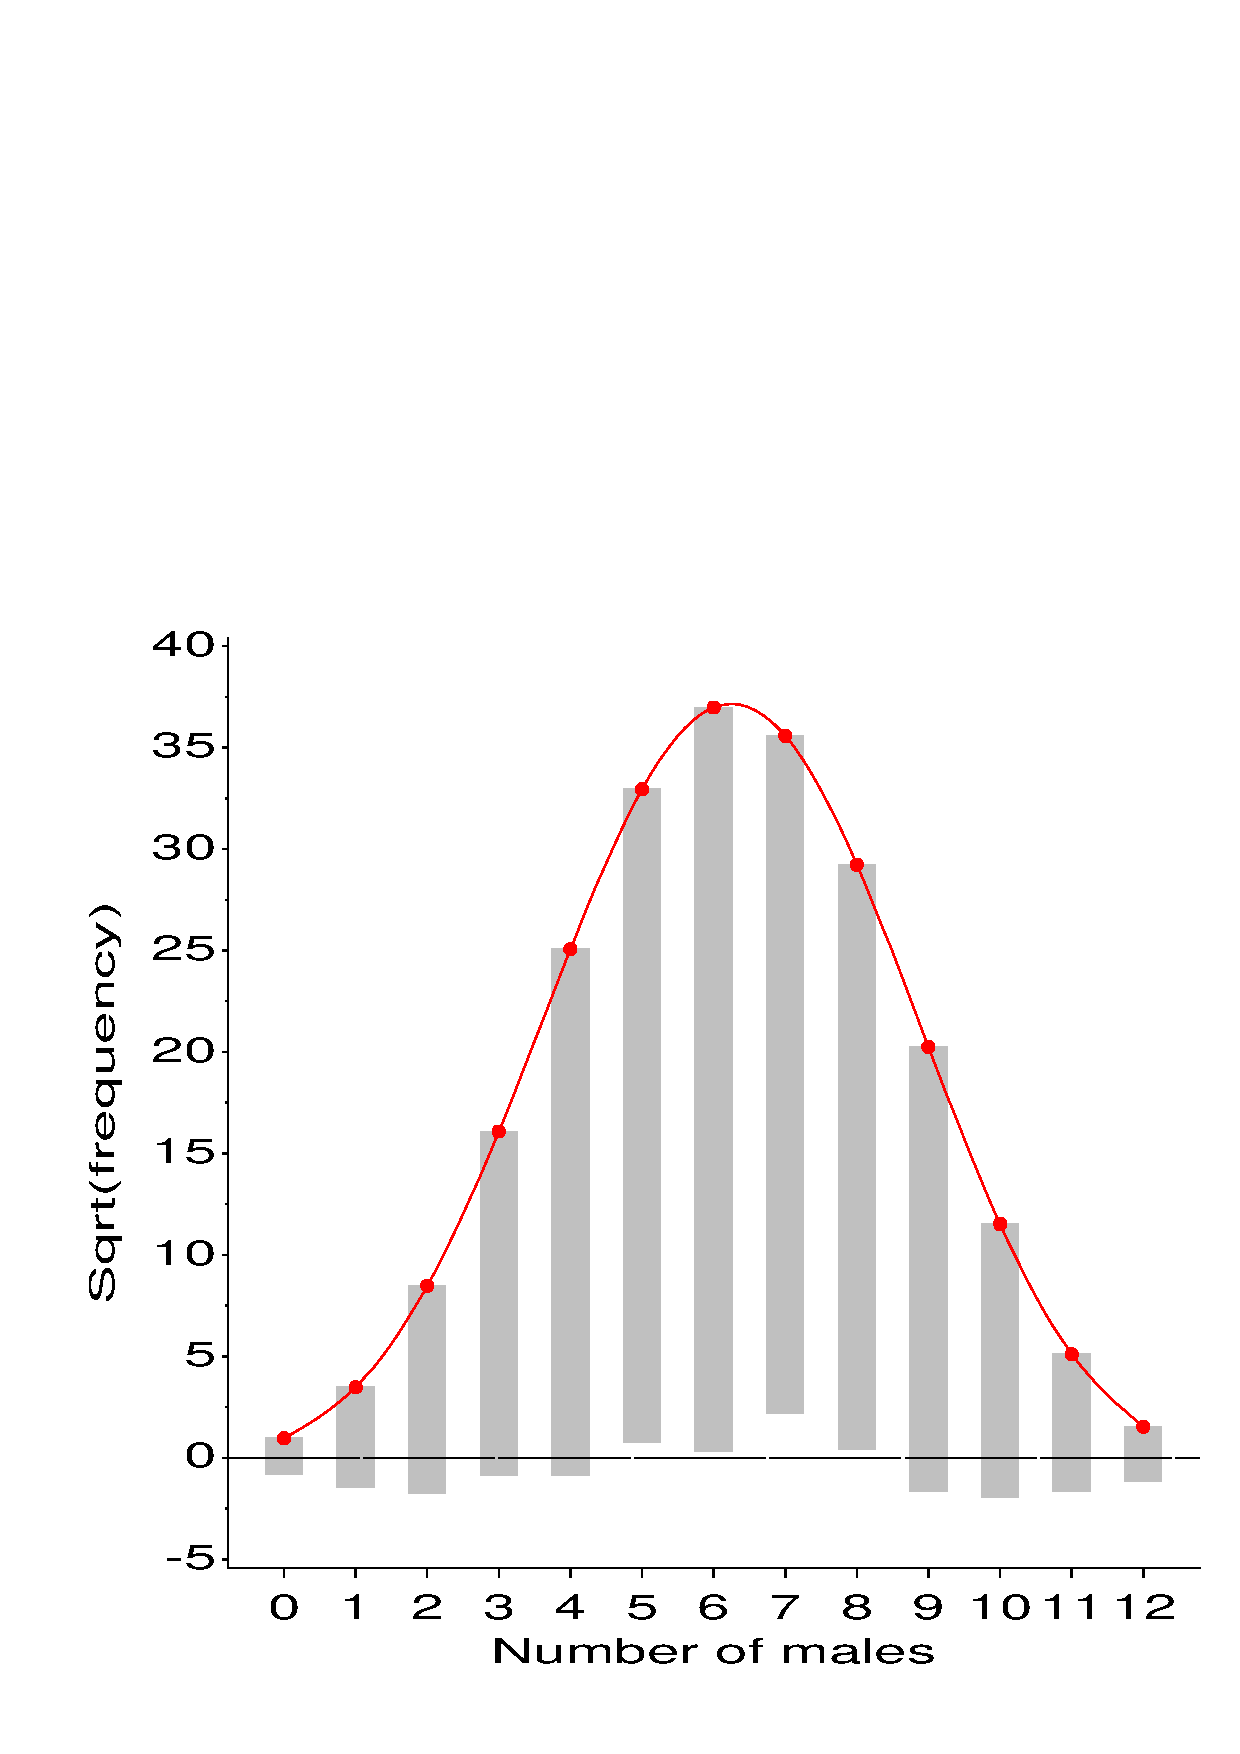
\includegraphics[width=1\linewidth]{saxony}\graphicsfile{ch2/fig/saxony.eps}{}
 \end{minipage}%
 \hfill
 \begin{minipage}[c]{.33\linewidth}
  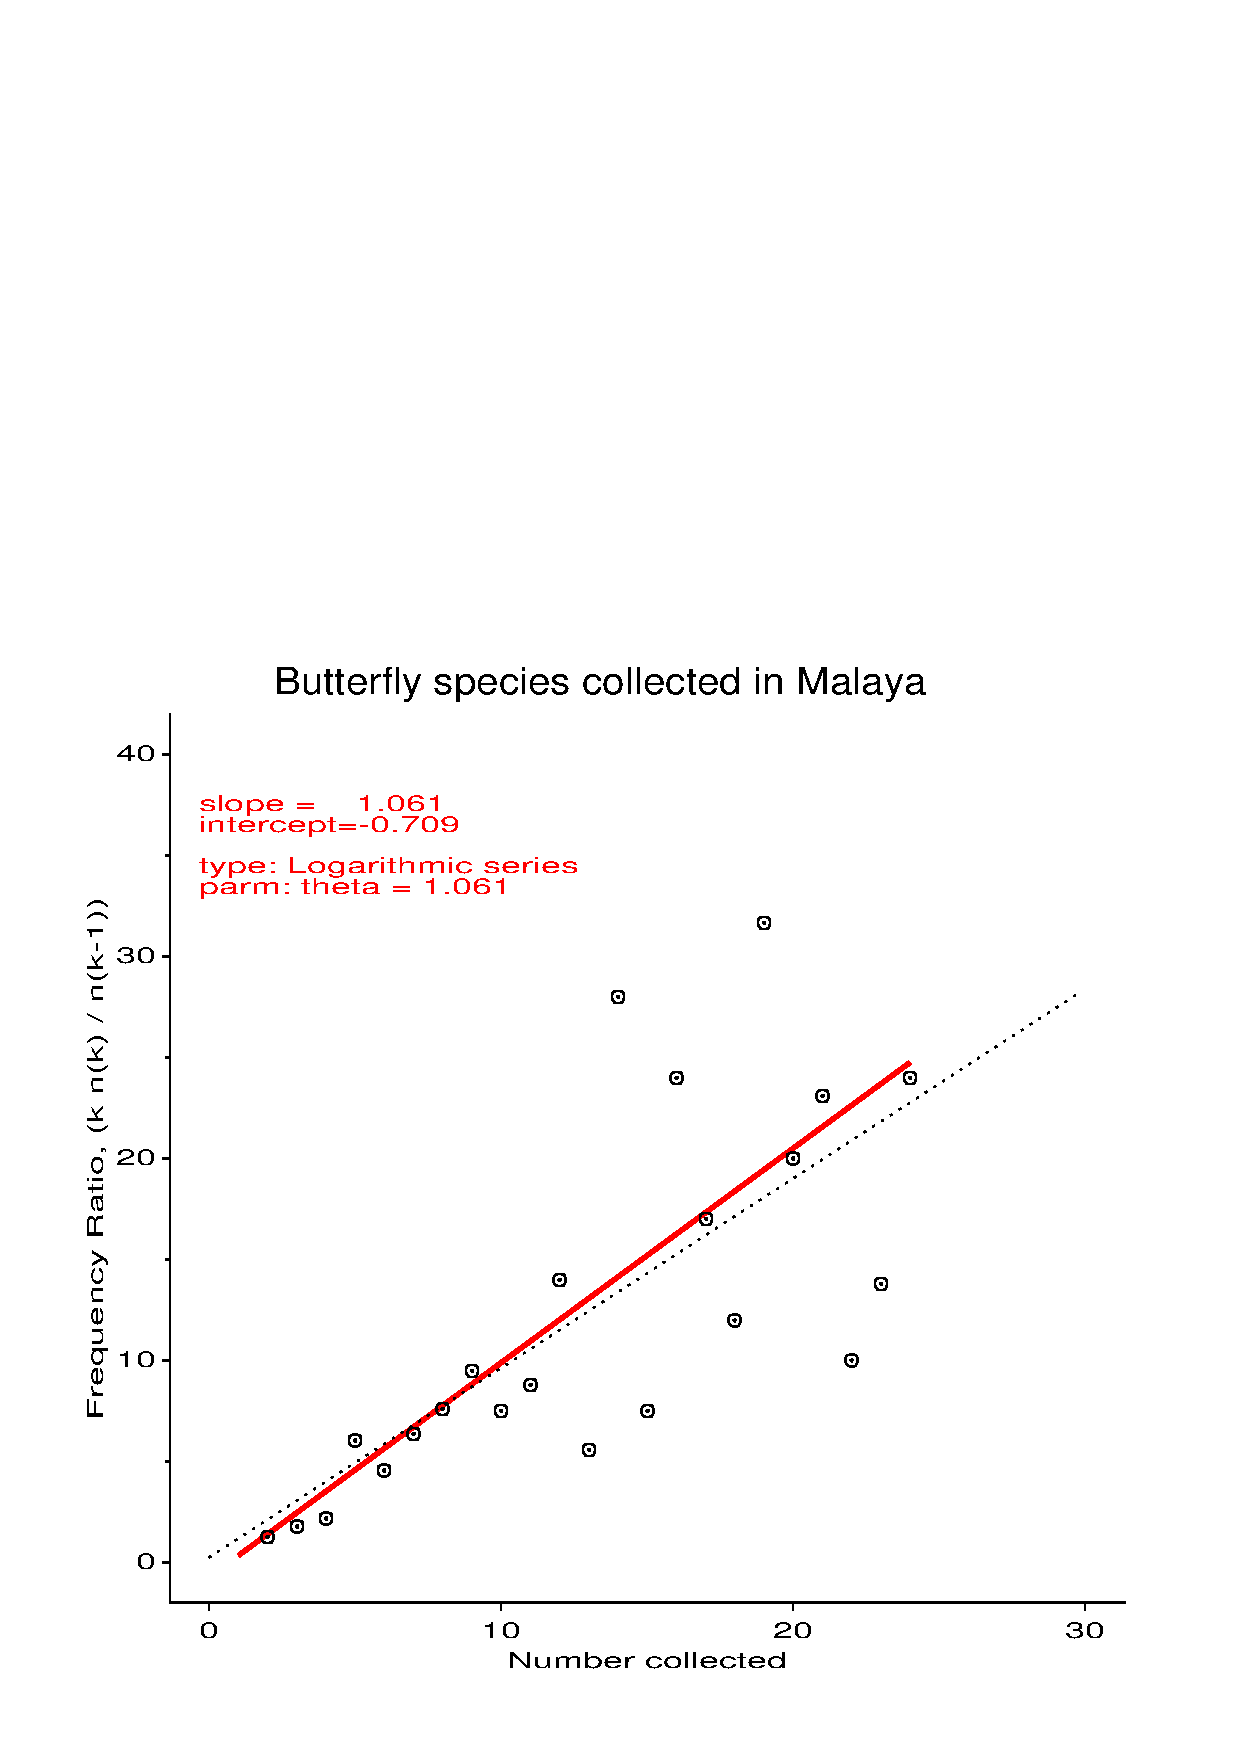
\includegraphics[width=1\linewidth]{orddemo3}\graphicsfile{ch2/fig/orddemo3.eps}{}
 \end{minipage}
 \hfill
 \begin{minipage}[c]{.33\linewidth}
  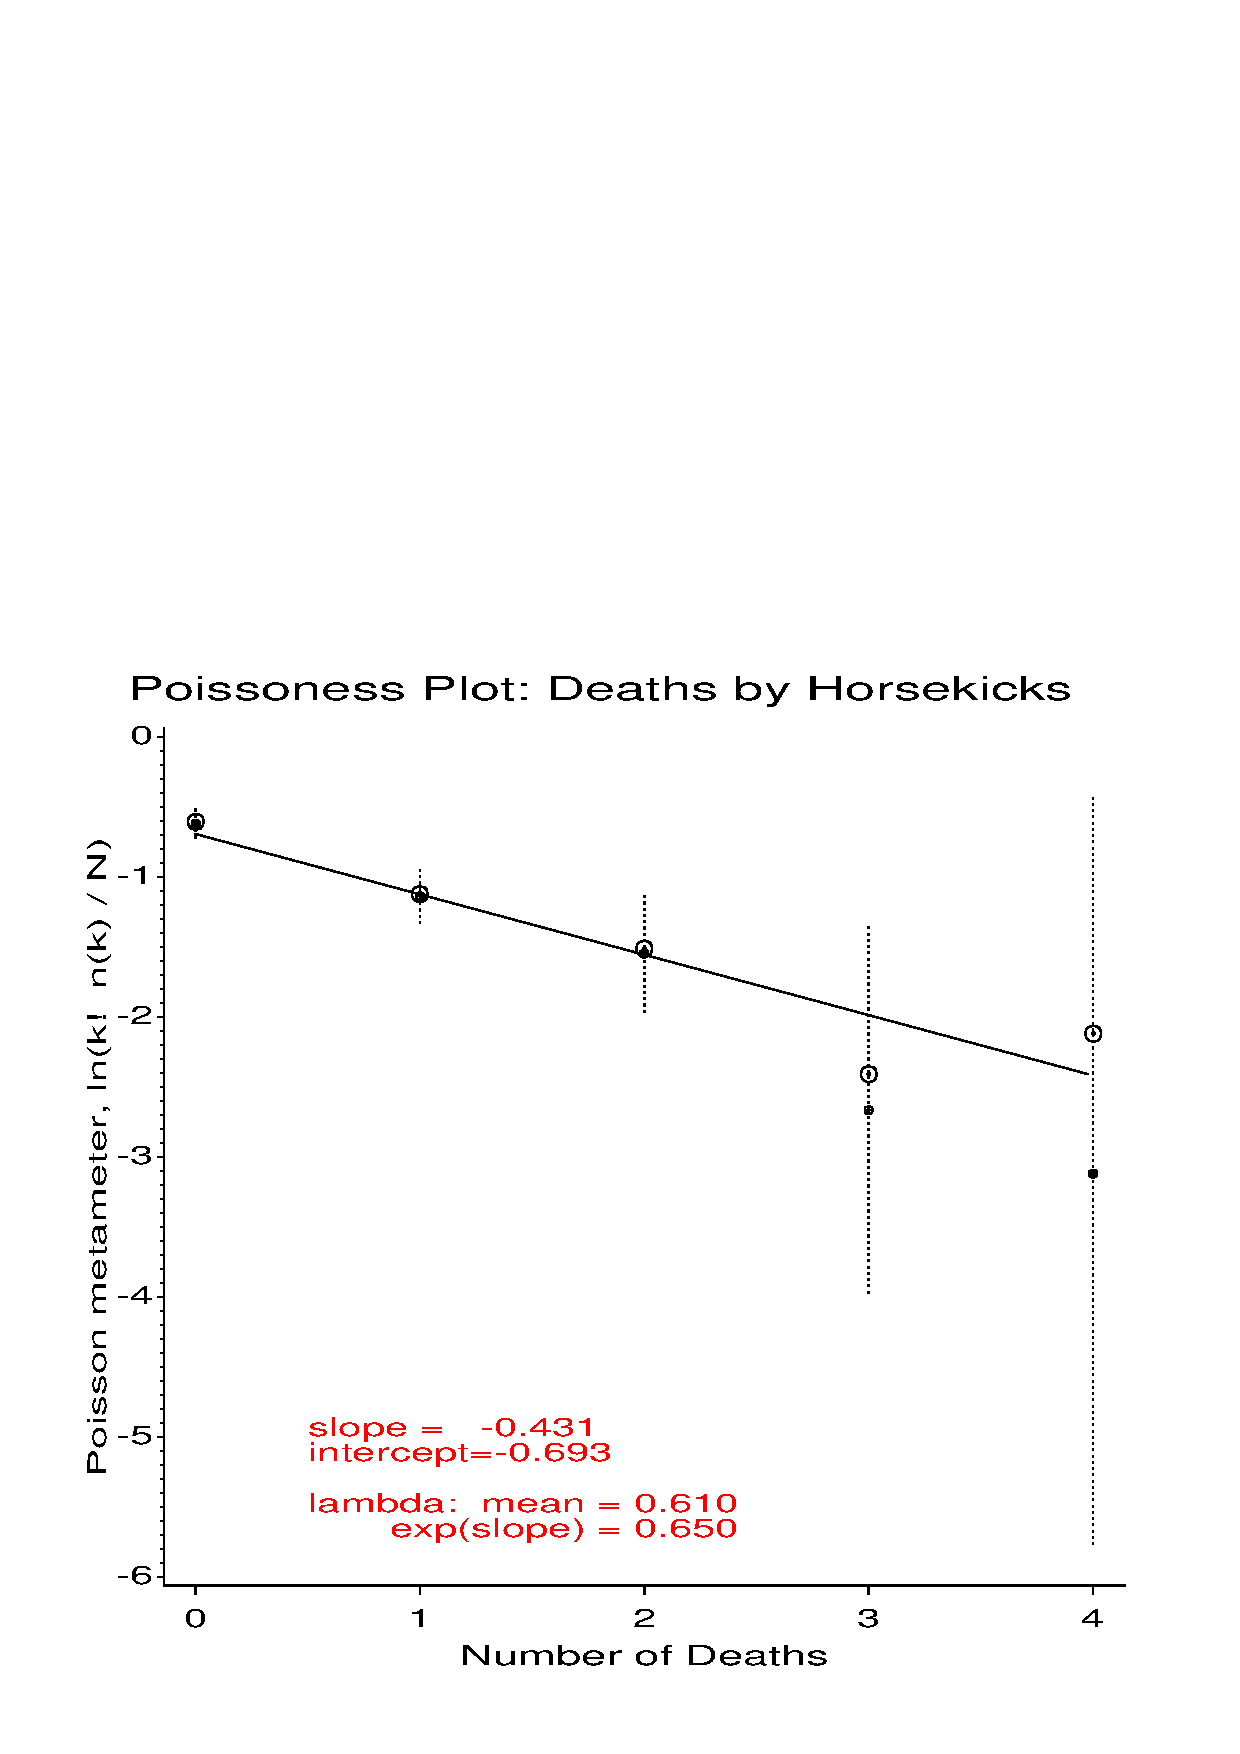
\includegraphics[width=1\linewidth]{poisdemo1}\graphicsfile{ch2/fig/poisdemo1.eps}{}
 \end{minipage}
\end{center}

		% visual table of contents

\chapterprelude{
Mosaic displays help to visualize the pattern of associations
among variables in two-way and larger tables.  Extensions of
this technique can reveal partial associations, marginal associations,
and shed light on the structure of \loglin\ models themselves.
}
% \minitoc
% \clearpage

\section{Introduction}\label{sec:mosaic-intro}
% \epigraph{Little boxes, on the hillside, little boxes made of ticky-tacky;\\
% Little boxes, little boxes, little boxes all the same.\\
% There's a green one and a pink one and a blue one and a yellow one;\\
% Little boxes, little boxes, and they all look just the same.}%
% {Written and composed by Malvina Renolds, recorded by Pete Seeger}

%\begin{comment}
\epigraph{%
Little boxes on the hillside,
little boxes made of ticky tacky, \\
Little boxes on the hillside,
little boxes all the same. \\
There's a green one and a pink one,
and a blue one and a yellow one, \\
And they're all made out of ticky tacky,
and they all look just the same.
}
{Words and music by Malvina Reynolds, \copyright Schroder Music Company 1962, 1990; recorded by Pete Seeger}
%\end{comment}

In \chref{ch:twoway}, we described a variety of graphical techniques
for visualizing the pattern of association in simple \ctabs.
These methods are somewhat specialized for particular
sizes and shapes of tables:
$2 \times 2$ tables (fourfold display),
$r \times c$ tables (tile plot, sieve diagram),
square tables (agreement charts),
$r \times 3$ tables (trilinear plots), and so forth.

This chapter describes the
\term{mosaic display} and related graphical methods
for \nway frequency tables, designed to show
various aspects of high-dimensional contingency tables in a hierarchical way.
These methods portray the
frequencies in an \nway
\ctab  by a collection of rectangular ``tiles''
whose size (area) is proportional to the cell frequency.
In this respect, the mosaic display is similar to the sieve diagram (\secref{sec:twoway-sieve}).
However, mosaic plots and related methods described here:
\begin{itemize}
\item generalize more readily to \nway tables.  One can usefully examine
3-way, 4-way and even larger tables, subject to the limitations
of resolution in any graph;
\item are intimately connected to \loglin models, generalized linear models
and generalized nonlinear models for frequency data;
\item provide a method for fitting a series of sequential \loglin
models to the various marginal totals of an \nway table; and
\item can be used to illustrate the relations among variables which
are fitted by various \loglin models.
\end{itemize}


\section{Two-way tables}\label{sec:mosaic-twoway}

The mosaic display
\citep{Friendly:92b,Friendly:94a,Friendly:97,HartiganKleiner:81,HartiganKleiner:84}
is like a grouped barchart,
where the heights (or widths) of the bars show the relative frequencies of one
variable, and widths (heights) of the sections in each bar show the
conditional frequencies of the second variable, given the first.
This gives an area-proportional visualization of the frequencies
composed of tiles corresponding to the cells created by successive
vertical and horizontal splits of rectangle, representing the total
frequency in the table.
%as shown in \figref{fig:mosaic31}.
% Additional variables can be displayed by dividing
The construction of the mosaic display, and what it reveals,
are most easily understood for two-way tables.

\begin{Example}[haireye2a]{Hair color and eye color}
Consider the data shown earlier in  \tabref{tab:hairdat},
showing the relation between hair color and eye color among students
in a statistics course.  The basic mosaic display for this $4 \times 4$
table is shown in \figref{fig:haireye-mos1}.

% Don't want to show the code for labeling_cells() here
\begin{knitrout}
\definecolor{shadecolor}{rgb}{1, 0.961, 0.933}\color{fgcolor}\begin{figure}[!htbp]

\centerline{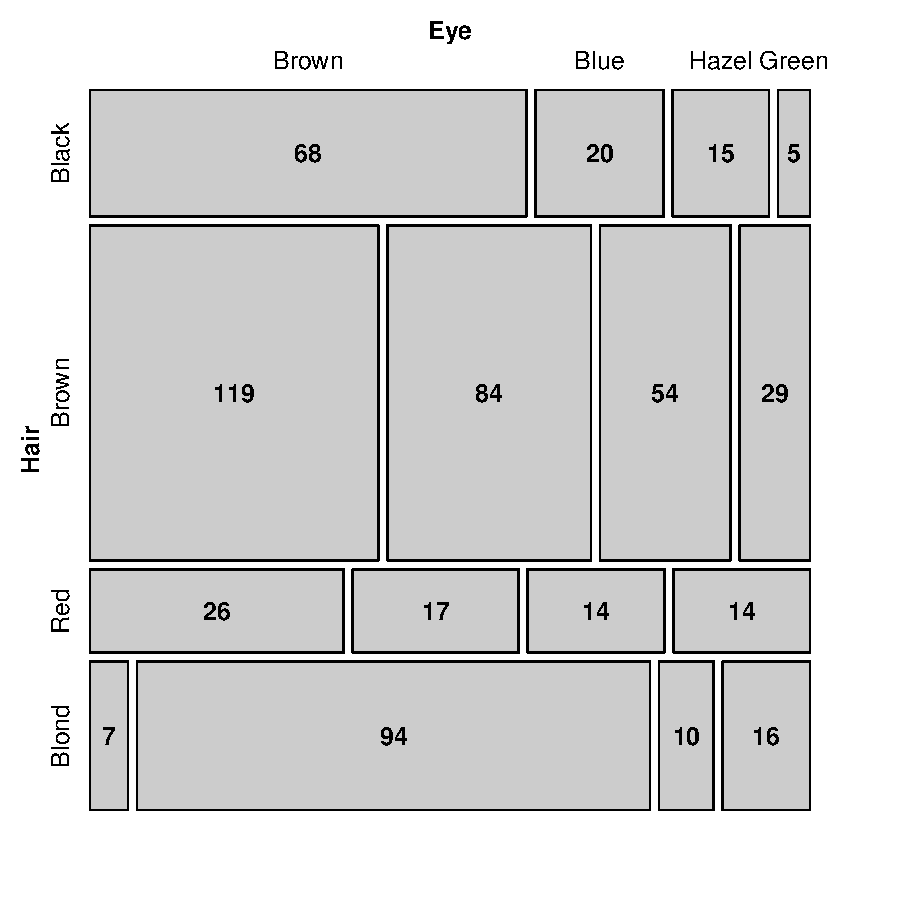
\includegraphics[width=.6\textwidth]{ch05/fig/haireye-mos1-1} }

\caption[Basic mosaic display for hair color and eye color data]{Basic mosaic display for hair color and eye color data.  The area of each rectangle is proportional to the observed frequency in that cell, shown as numbers.\label{fig:haireye-mos1}}
\end{figure}


\end{knitrout}

\begin{knitrout}
\definecolor{shadecolor}{rgb}{1, 0.961, 0.933}\color{fgcolor}\begin{kframe}
\begin{alltt}
\hlstd{> }\hlkwd{data}\hlstd{(HairEyeColor,} \hlkwc{package} \hlstd{=} \hlstr{"datasets"}\hlstd{)}
\hlstd{> }\hlstd{haireye} \hlkwb{<-} \hlkwd{margin.table}\hlstd{(HairEyeColor,} \hlnum{1} \hlopt{:} \hlnum{2}\hlstd{)}
\hlstd{> }\hlkwd{mosaic}\hlstd{(haireye,} \hlkwc{labeling} \hlstd{= labeling_values)}
\end{alltt}
\end{kframe}
\end{knitrout}

For such a two-way table, the mosaic in \figref{fig:haireye-mos1} is constructed
by first dividing a unit square in proportion to the marginal
totals of one variable, say, Hair color.

For these data, the marginal frequencies and proportions of Hair color are calculated below:
\begin{knitrout}
\definecolor{shadecolor}{rgb}{1, 0.961, 0.933}\color{fgcolor}\begin{kframe}
\begin{alltt}
\hlstd{> }\hlstd{(hair} \hlkwb{<-} \hlkwd{margin.table}\hlstd{(haireye,} \hlnum{1}\hlstd{))}
\end{alltt}
\begin{verbatim}
Hair
Black Brown   Red Blond 
  108   286    71   127 
\end{verbatim}
\begin{alltt}
\hlstd{> }\hlkwd{prop.table}\hlstd{(hair)}
\end{alltt}
\begin{verbatim}
Hair
  Black   Brown     Red   Blond 
0.18243 0.48311 0.11993 0.21453 
\end{verbatim}
\end{kframe}
\end{knitrout}

% Construct the figures first, then explain the details in separate chunks
% try using out.height rather than out.width='.49\\textwidth'
\begin{knitrout}
\definecolor{shadecolor}{rgb}{1, 0.961, 0.933}\color{fgcolor}\begin{figure}[!htbp]

\centerline{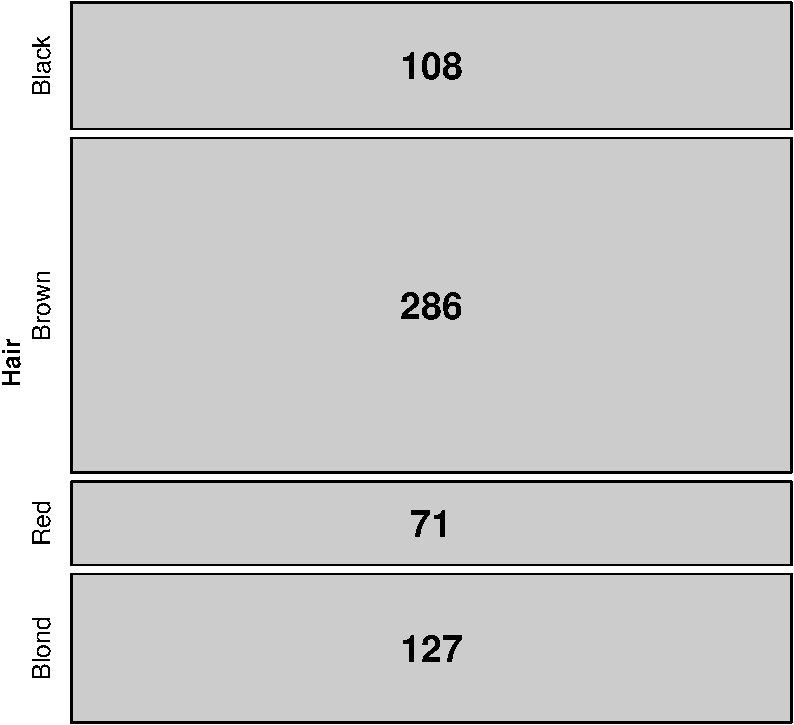
\includegraphics[width=.49\textwidth]{ch05/fig/haireye-mos4-1} 
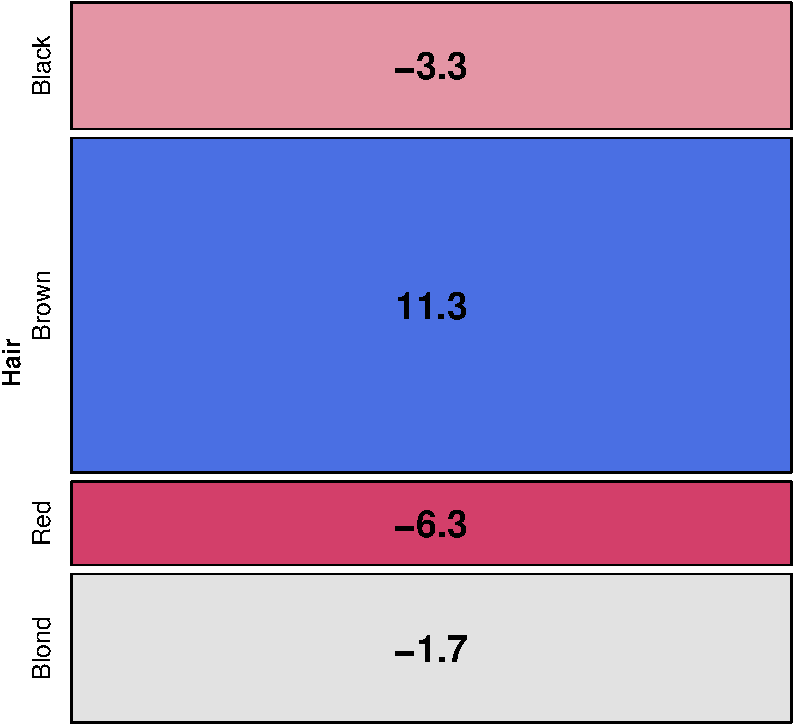
\includegraphics[width=.49\textwidth]{ch05/fig/haireye-mos4-2} }

\caption[First step in constructing a mosaic display]{First step in constructing a mosaic display. Left: splitting the unit square according to frequencies of hair color; right: shading the tiles according to residuals from a model of equal marginal probabilities.\label{fig:haireye-mos4}}
\end{figure}


\end{knitrout}
% \begin{figure}[htb]
%   \centering
%   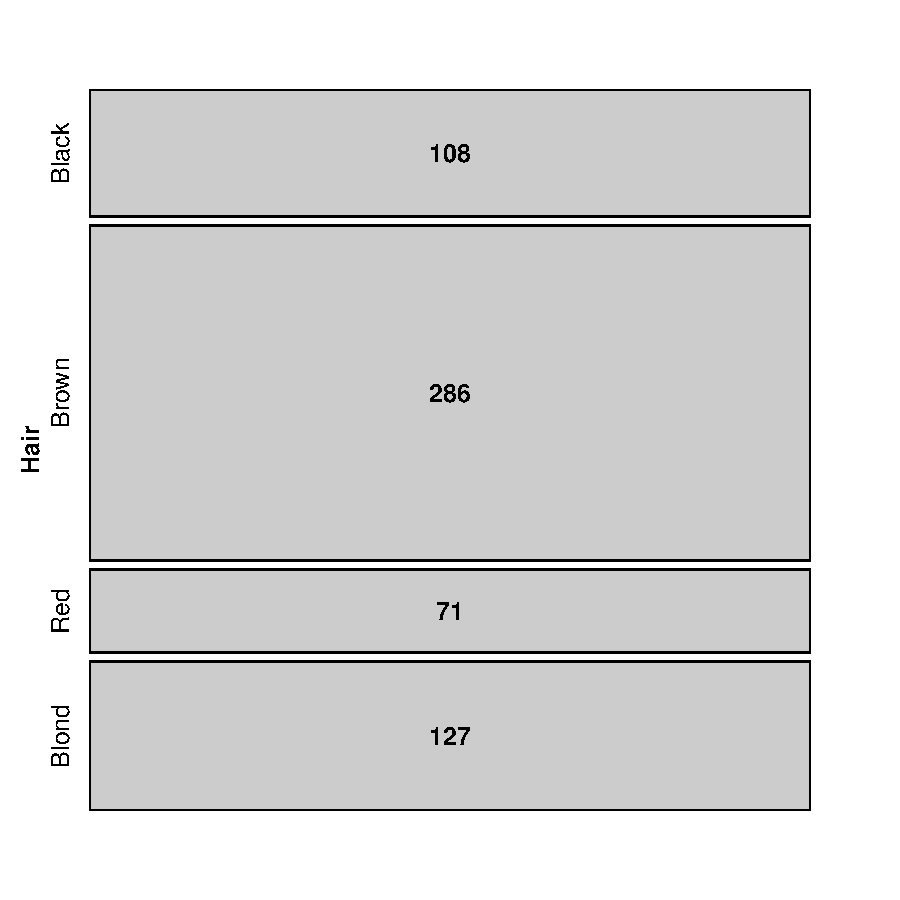
\includegraphics[width=.4\textwidth]{ch05/fig/haireye-mos41}
%   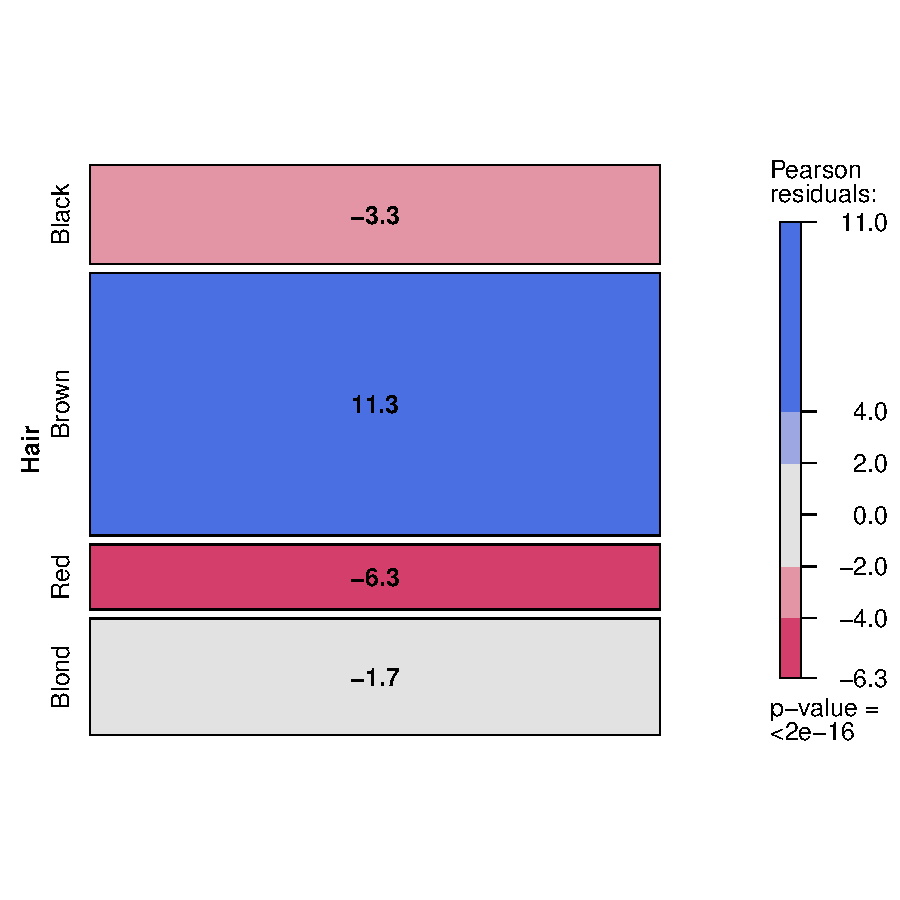
\includegraphics[width=.59\textwidth]{ch05/fig/haireye-mos42}
%   \caption{First step in constructing a mosaic display. Left: splitting the unit square according to frequencies of hair color; right: shading the tiles according to residuals from a model of equal marginal probabilities.}
%   \label{fig:haireye-mos4}
% \end{figure}
% \TODO{Resize these figures so they are both of the same height. Maybe have to
% manually do the figure environment here or use pdfcrop, or legend=FALSE
% }

These frequencies can be shown as the mosaic for the first variable (hair color),
with the unit square split according to the marginal proportions
as in \figref{fig:haireye-mos4} (left).
The rectangular tiles are then shaded to show the residuals (deviations)
from a particular model as shown in the right panel of \figref{fig:haireye-mos4}.
The details of the calculations for shading are:

\begin{itemize}
\item The one-way table of marginal totals can be fit to a model, in this
case, the (implausible) model that all hair colors are equally probable.  This model
has expected frequencies $m_i = 592/4 = 148$:
\begin{knitrout}
\definecolor{shadecolor}{rgb}{1, 0.961, 0.933}\color{fgcolor}\begin{kframe}
\begin{alltt}
\hlstd{> }\hlstd{expected} \hlkwb{<-} \hlkwd{rep}\hlstd{(}\hlkwd{sum}\hlstd{(hair)} \hlopt{/} \hlnum{4}\hlstd{,} \hlnum{4}\hlstd{)}
\hlstd{> }\hlkwd{names}\hlstd{(expected)} \hlkwb{<-} \hlkwd{names}\hlstd{(hair)}
\hlstd{> }\hlstd{expected}
\end{alltt}
\begin{verbatim}
Black Brown   Red Blond 
  148   148   148   148 
\end{verbatim}
\end{kframe}
\end{knitrout}
\item The Pearson residuals from this model, $r_i = ( n_i - m_i ) / \sqrt{m_i}$, are:
\begin{knitrout}
\definecolor{shadecolor}{rgb}{1, 0.961, 0.933}\color{fgcolor}\begin{kframe}
\begin{alltt}
\hlstd{> }\hlstd{(residuals} \hlkwb{<-} \hlstd{(hair} \hlopt{-} \hlstd{expected)} \hlopt{/} \hlkwd{sqrt}\hlstd{(expected))}
\end{alltt}
\begin{verbatim}
Hair
  Black   Brown     Red   Blond 
-3.2880 11.3435 -6.3294 -1.7262 
\end{verbatim}
\end{kframe}
\end{knitrout}
and these values are shown by color and shading as shown in the legend
in \figref{fig:haireye-mos8}.
The high positive value for Brown hair indicates that people
with brown hair are much more frequent in this sample than
the equiprobability model would predict; the large negative residual
for Red hair shows that red heads are much less common.  Further details
of the schemes for shading are described below, but essentially we use
increasing intensities of blue (red) for positive (negative) residuals.
\end{itemize}

In the next step, the rectangle for each Hair color is subdivided in proportion
to the \emph{relative} (conditional) frequencies of the second variable---
Eye color, giving the following conditional row proportions:

\begin{knitrout}
\definecolor{shadecolor}{rgb}{1, 0.961, 0.933}\color{fgcolor}\begin{kframe}
\begin{alltt}
\hlstd{> }\hlkwd{round}\hlstd{(}\hlkwd{addmargins}\hlstd{(}\hlkwd{prop.table}\hlstd{(haireye,} \hlnum{1}\hlstd{),} \hlnum{2}\hlstd{),} \hlnum{3}\hlstd{)}
\end{alltt}
\begin{verbatim}
       Eye
Hair    Brown  Blue Hazel Green   Sum
  Black 0.630 0.185 0.139 0.046 1.000
  Brown 0.416 0.294 0.189 0.101 1.000
  Red   0.366 0.239 0.197 0.197 1.000
  Blond 0.055 0.740 0.079 0.126 1.000
\end{verbatim}
\end{kframe}
\end{knitrout}
The proportions in each row determine the width of the tiles in the second mosaic display in \figref{fig:haireye-mos8}.

\begin{knitrout}
\definecolor{shadecolor}{rgb}{1, 0.961, 0.933}\color{fgcolor}\begin{figure}[!htbp]

\centerline{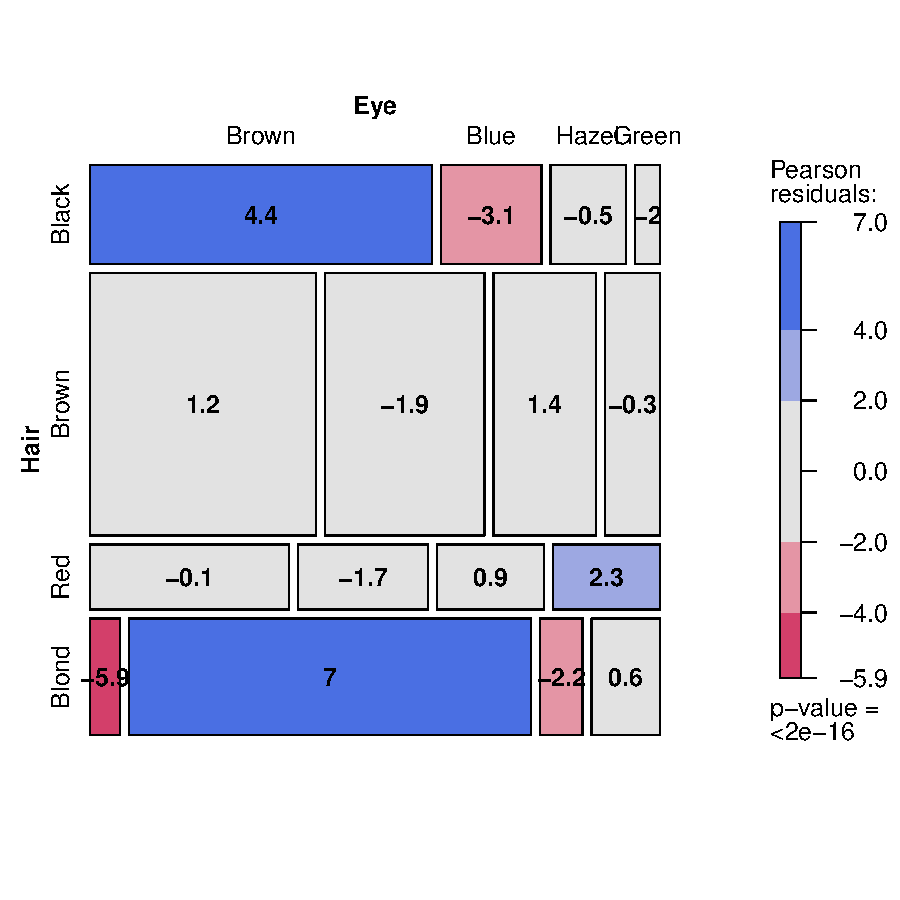
\includegraphics[width=.6\textwidth]{ch05/fig/haireye-mos8-1} }

\caption[Second step in constructing the mosaic display]{Second step in constructing the mosaic display.  Each rectangle for hair color is subdivided in proportion to the relative frequencies of eye color, and the tiles are shaded in relation to residuals from the model of independence.\label{fig:haireye-mos8}}
\end{figure}


\end{knitrout}

\begin{itemize}
\item Again, the cells are shaded in relation to standardized Pearson
residuals, \(r_{ij} = (n_{ij} - m_{ij}) / \sqrt { m_{ij} }\),
from a model.  For a two-way table, the model is that Hair color and
Eye color are independent in the population from which this sample
was drawn.  These residuals are calculated as shown below using
\func{independence\_table} to calculate the expected values $m_{ij}$ under this
model ($m_{ij} = n_{++} \pi_{i+} \pi_{+j}$):
\begin{knitrout}
\definecolor{shadecolor}{rgb}{1, 0.961, 0.933}\color{fgcolor}\begin{kframe}
\begin{alltt}
\hlstd{> }\hlstd{exp} \hlkwb{<-} \hlkwd{independence_table}\hlstd{(haireye)}
\hlstd{> }\hlstd{resids} \hlkwb{<-} \hlstd{(haireye} \hlopt{-} \hlstd{exp)} \hlopt{/} \hlkwd{sqrt}\hlstd{(exp)}
\hlstd{> }\hlkwd{round}\hlstd{(resids,} \hlnum{2}\hlstd{)}
\end{alltt}
\begin{verbatim}
       Eye
Hair    Brown  Blue Hazel Green
  Black  4.40 -3.07 -0.48 -1.95
  Brown  1.23 -1.95  1.35 -0.35
  Red   -0.07 -1.73  0.85  2.28
  Blond -5.85  7.05 -2.23  0.61
\end{verbatim}
\end{kframe}
\end{knitrout}
\item Thus, in \figref{fig:haireye-mos8},
the two tiles shaded deep blue correspond to the two
cells, (Black, Brown) and (Blond, Blue), whose residuals are
greater than $+4$, indicating much greater frequency in those
cells than would be found if Hair color and Eye color were
independent.
The tile shaded deep red, (Blond, Brown),
corresponds to the largest negative residual = $-5.85$, indicating this combination
is extremely rare under the hypothesis of independence.
\item The overall Pearson \chisq{} statistic for the independence model
is just the
sum of squares of the residuals, with degrees of freedom $(r-1) \times (c-1)$.
\begin{knitrout}
\definecolor{shadecolor}{rgb}{1, 0.961, 0.933}\color{fgcolor}\begin{kframe}
\begin{alltt}
\hlstd{> }\hlstd{(chisq} \hlkwb{<-} \hlkwd{sum}\hlstd{(resids} \hlopt{^} \hlnum{2}\hlstd{))}
\end{alltt}
\begin{verbatim}
[1] 138.29
\end{verbatim}
\begin{alltt}
\hlstd{> }\hlstd{(df} \hlkwb{<-} \hlkwd{prod}\hlstd{(}\hlkwd{dim}\hlstd{(haireye)} \hlopt{-} \hlnum{1}\hlstd{))}
\end{alltt}
\begin{verbatim}
[1] 9
\end{verbatim}
\begin{alltt}
\hlstd{> }\hlkwd{pchisq}\hlstd{(chisq, df,} \hlkwc{lower.tail} \hlstd{=} \hlnum{FALSE}\hlstd{)}
\end{alltt}
\begin{verbatim}
[1] 2.3253e-25
\end{verbatim}
\end{kframe}
\end{knitrout}
\item These results are of course identical to what \func{chisq.test}
  provides. Note that the latter can be used to retrieve the residuals:
\begin{knitrout}
\definecolor{shadecolor}{rgb}{1, 0.961, 0.933}\color{fgcolor}\begin{kframe}
\begin{alltt}
\hlstd{> }\hlkwd{chisq.test}\hlstd{(haireye)}
\end{alltt}
\begin{verbatim}

	Pearson's Chi-squared test

data:  haireye
X-squared = 138.29, df = 9, p-value < 2.2e-16
\end{verbatim}
\begin{alltt}
\hlstd{> }\hlkwd{round}\hlstd{(}\hlkwd{residuals}\hlstd{(}\hlkwd{chisq.test}\hlstd{(haireye)),} \hlnum{2}\hlstd{)}
\end{alltt}
\begin{verbatim}
       Eye
Hair    Brown  Blue Hazel Green
  Black  4.40 -3.07 -0.48 -1.95
  Brown  1.23 -1.95  1.35 -0.35
  Red   -0.07 -1.73  0.85  2.28
  Blond -5.85  7.05 -2.23  0.61
\end{verbatim}
\end{kframe}
\end{knitrout}
\end{itemize}
\end{Example}

\subsubsection{Shading levels}

A variety of schemes for shading the tiles are available in the
strucplot framework (\secref{sec:mosaic-strucplot}),
but the simplest (and default) shading patterns for the tiles are based on
the sign and magnitude of the
standardized Pearson residuals, using shades of blue for positive residuals
and red for negative residuals, and two threshold values for their magnitudes,
$|r_{ij}| > 2$ and $|r_{ij}| > 4$.

Because the standardized residuals are approximately unit-normal $N(0,1)$
values,  this corresponds to highlighting cells whose
residuals are \emph{individually} significant at approximately
the .05 and .0001 level, respectively.
Other shading schemes described later provide tests of significance,
but the main purpose  of highlighting cells is to draw attention to the \emph{pattern}
of departures of the data from the assumed model of independence.

\subsubsection{Interpretation and reordering}

To interpret the association between Hair color and Eye color,
consider the pattern of positive (blue) and negative (red)
tiles in the mosaic display.
We interpret positive values as showing cells whose observed frequency
is substantially greater than would be found under independence;
negative values indicate cells which occur less often than
under independence.

The interpretation can often be enhanced by reordering the rows or columns
of the two-way table so that the residuals have an \emph{opposite
corner} pattern of signs.  This usually helps us interpret any systematic
patterns of association in terms of the ordering of the row and column
categories.

In this example, a more direct interpretation can be achieved by
reordering the Eye colors as shown in
\figref{fig:haireye-mos9}.
Note that in this rearrangement
both hair colors and eye colors are ordered from dark to light,
suggesting an overall interpretation of the association
between Hair color and Eye color.

\begin{knitrout}
\definecolor{shadecolor}{rgb}{1, 0.961, 0.933}\color{fgcolor}\begin{kframe}
\begin{alltt}
\hlstd{> }\hlcom{# re-order Eye colors from dark to light}
\hlstd{> }\hlstd{haireye2} \hlkwb{<-} \hlkwd{as.table}\hlstd{(haireye[,} \hlkwd{c}\hlstd{(}\hlstr{"Brown"}\hlstd{,} \hlstr{"Hazel"}\hlstd{,} \hlstr{"Green"}\hlstd{,} \hlstr{"Blue"}\hlstd{)])}
\hlstd{> }\hlkwd{mosaic}\hlstd{(haireye2,} \hlkwc{shade} \hlstd{=} \hlnum{TRUE}\hlstd{)}
\end{alltt}
\end{kframe}\begin{figure}[!htbp]

\centerline{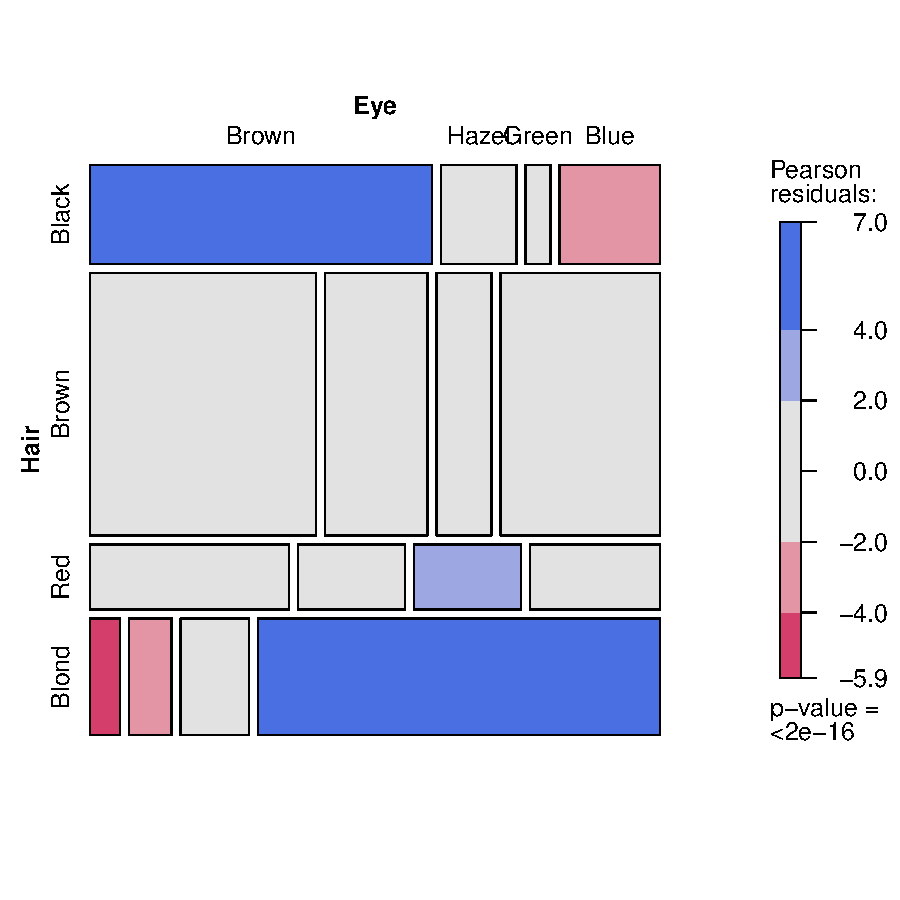
\includegraphics[width=.6\textwidth]{ch05/fig/haireye-mos9-1} }

\caption[Two-way mosaic for Hair color and Eye color, reordered]{Two-way mosaic for Hair color and Eye color, reordered. The Eye colors were reordered from dark to light, enhancing the interpretation.\label{fig:haireye-mos9}}
\end{figure}


\end{knitrout}

In general, the levels of a factor in mosaic displays
are often best reordered by
arranging them according to their scores on the first (largest)
\emph{correspondence analysis} dimension \citep{Friendly:94a};
see \chref{ch:corresp} for details.
\citet{FriendlyKwan:02:effect} use this as one example of
\term{effect ordering} for data displays, illustrated in \chref{ch:intro}.

Thus, the mosaic in \figref{fig:haireye-mos9} shows that the association between Hair and Eye color
is essentially that:
\begin{itemize*}
\item people with dark hair tend to have dark eyes,
\item those with light hair tend to have light eyes
\item people with red hair and hazel eyes do not quite fit this pattern
\end{itemize*}
\ixe{Hair color and eye color}

\section{The strucplot framework}\label{sec:mosaic-strucplot}
Mosaic displays have much in common with sieve plots and association plots
described in \chref{ch:twoway} and with related graphical methods
such as \term{doubledecker plots} described later in this chapter.
The main idea is to visualize a \ctab of frequencies by ``tiles'' corresponding
to the table cells arranged in rectangular form.
For \mway tables with more than two factors,
the variables are nested into rows and columns using recursive
conditional splits, given the table margins. The result is a
``flat'' representation that can be visualized in
ways similar to a two-dimensional representation of a table.
The \func{structable} function described in \secref{sec:structable} gives the tabular
version of a strucplot.  The description below follows \citet{MeyerZeileisHornik:2006}, also
included as a vignette,
(accessible from \R as \code{vignette("strucplot", pkg = "vcd")}), in \pkg{vcd}.

Rather than implementing each of these methods separately, the
\term{strucplot framework} in the \Rpackage{vcd} provides a
general class of methods of which these are all instances.
This framework defines a class of conditional displays which allows
for granular control of graphical appearance aspects, including:

\begin{itemize*}
\item the content of the tiles, e.g., observed or expected frequencies
\item the split direction for each dimension, horizontal or vertical
\item the graphical parameters of the tiles' content, e.g., color or other visual attributes
\item the spacing between the tiles
\item the labeling of the tiles
\end{itemize*}

\begin{figure}
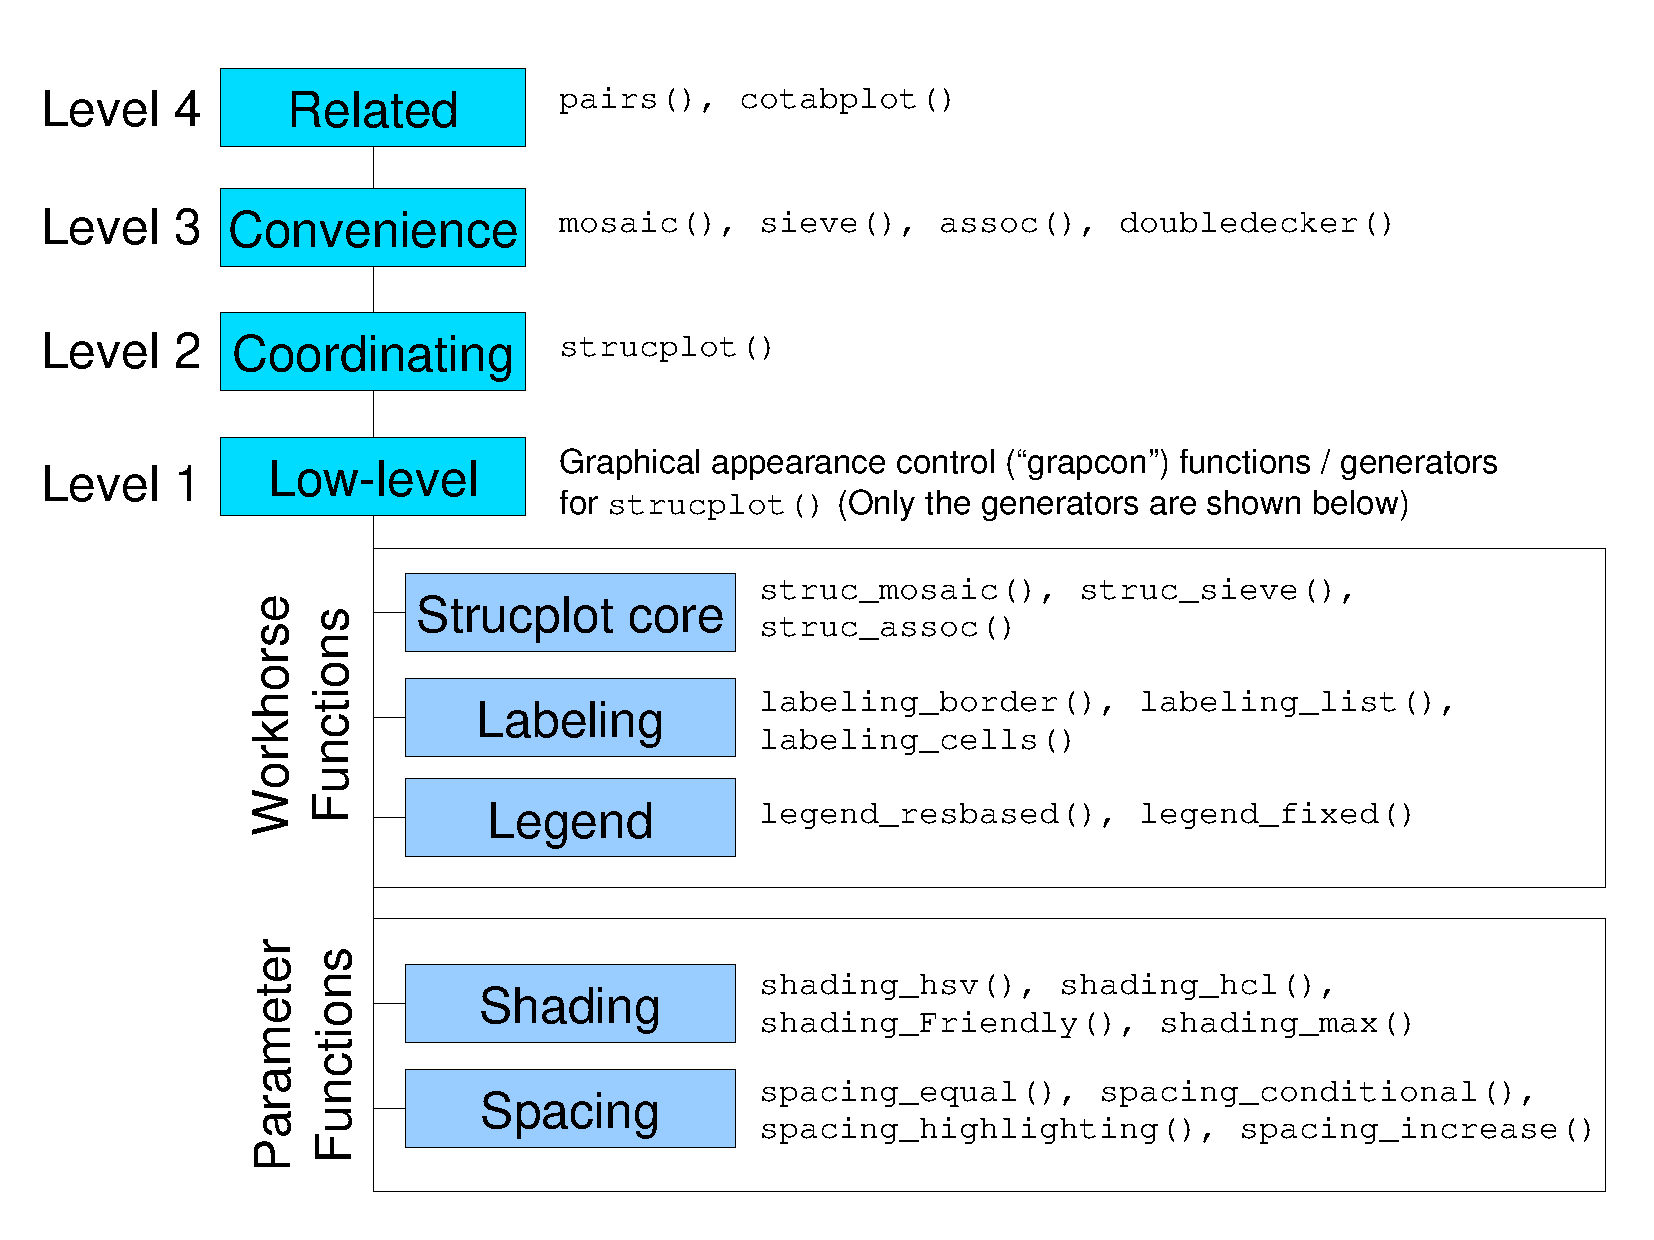
\includegraphics[width=.8\textwidth]{ch05/fig/struc}
\caption{Components of the strucplot framework. High level functions use those at lower levels to provide a general system for tile-based plots of frequency tables.}
\label{fig:struc}
\end{figure}

The strucplot framework is highly modularized: \figref{fig:struc}
shows the hierarchical relationship between the various components.
For the most part, you will use directly the convenience and related
functions at the top of the diagram, but it is more convenient to
describe the framework from the bottom up.

\begin{table}[!htb]
{\small
  \begin{tabular}{|l|l|l|}
    \hline
\tableheader
    \textbf{Group} & \textbf{Grapcon generator} & \textbf{Description}\\\hline
    strucplot & \func{struc\_assoc} & core function for association plots\\
    core      & \func{struc\_mosaic} & core function for mosaic plots
    (also used for tile plots)\\
              & \func{struc\_sieve} & core function for sieve plots\\
              \hline\hline
     labeling & \func{labeling\_border} & border labels\\
              & \func{labeling\_cboxed} & centered labels with
              boxes, all labels clipped,\\
              && and on top and left border\\
              & \func{labeling\_cells} & cell labels\\
              & \func{labeling\_conditional} & border labels
                                                  for conditioning variables\\
              && and cell labels for conditioned variables\\
              & \func{labeling\_doubledecker} & draws labels for
              doubledecker plot\\
              & \func{labeling\_lboxed} & left-aligned labels with boxes\\
              & \func{labeling\_left} & left-aligned border labels\\
              & \func{labeling\_left2} & left-aligned border
              labels, all labels on top and left border\\
              & \func{labeling\_list} & draws a list of labels
              under the plot\\
              & \func{labeling\_residuals} & show residuals in cells\\
              & \func{labeling\_value} & show values (observed, expected) in cells\\
              \hline\hline
     shading  & \func{shading\_binary} & visualizes the sign of the  residuals\\
              & \func{shading\_Friendly} & implements Friendly
              shading (based on HSV colors)\\
              & \func{shading\_hcl} & shading based on HCL colors\\
              & \func{shading\_hsv} & shading based on HSV colors\\
              & \func{shading\_max} & shading visualizing the
              maximum test statistic\\ && (based on HCL colors)\\
              & \func{shading\_sieve} & implements Friendly
              shading customized for sieve plots\\ && (based on HCL colors)\\
              \hline\hline
     spacing  & \func{spacing\_conditional} & increasing spacing
              for conditioning variables,\\&& equal spacing for
              conditioned variables\\
              & \func{spacing\_dimequal} & equal spacing for each dimension\\
              & \func{spacing\_equal} & equal spacing for all dimensions\\
              & \func{spacing\_highlighting} & increasing spacing,
              last dimension set to zero\\
              & \func{spacing\_increase} & increasing spacing\\\hline\hline
     legend   & \func{legend\_fixed} & creates a fixed number of
              bins (similar to \func{mosaicplot})\\
              & \func{legend\_resbased} & suitable for an
              arbitrary number of bins\\&& (also for continuous shadings)\\\hline

  \end{tabular}
  \caption{Available graphical appearance control (grapcon) generators in the strucplot framework}
  \label{tab:grapcons}
}
\end{table}


\begin{enumerate}

\item On the lowest level, there are several groups of workhorse and
parameter functions that directly or indirectly influence the final
appearance of the plot (see Table \ref{tab:grapcons} for an overview).
These are examples of
\emph{\underline{gr}aphical \underline{ap}pearance \underline{con}trol} functions
(called \term{grapcon functions}).
They are created by generating functions
(\emph{grapcon generators}), allowing
flexible parameterization and extensibility (Figure~\ref{fig:struc}
only shows the generators). The generator names
follow the naming convention \code{\textit{group\_foo}()},
where \code{\textit{group}} reflects the group the
generators belong to (strucplot core, labeling,
legend, shading, or spacing).
  \begin{itemize*}
  \item The workhorse functions (created by
  \code{struc\_\textit{foo}()}) are
  \code{labeling\_\textit{foo}()}, and \code{legend\_\textit{foo}()}.
  These functions
  directly produce graphical output (i.e., ``add ink to the canvas''),
  for labels and legends respectively.
  \item The parameter functions
  (created by \code{spacing\_\textit{foo}()} and \code{shading\_\textit{foo}()}) compute
  graphical parameters used by the others. The grapcon functions returned by
  \code{struc\_\textit{foo}()} implement the core functionality,
  creating the tiles and their
  content.
  \end{itemize*}

\item On the second level of the framework, a suitable combination
of the low-level grapcon functions (or, alternatively, corresponding generating functions)
is passed as ``hyperparameters'' to \func{strucplot}.
This central function
sets up the graphical layout using grid viewports,
%(see Figure~\ref{fig:layout}),
and coordinates the specified core, labeling, shading, and spacing functions to produce
the plot.

\item On the third level, \pkg{vcd} provides
several convenience functions such as \func{mosaic},
\func{sieve}, \func{assoc}, \func{tile}, and \func{doubledecker} which
interface to \func{strucplot} through sensible parameter defaults
and support for model formulae.

\item Finally, on the fourth
level, there are ``related'' \pkg{vcd} functions (such as \func{cotabplot}
and the \func{pairs} methods for table objects)
arranging collections of plots of the strucplot
framework into more complex displays (e.g., by means of panel functions).
\end{enumerate}

\subsection{Shading schemes}\label{sec:mosaic-shading}


Unlike other graphics functions in base \R, the strucplot framework
allows almost full control over the graphical parameters of all plot elements. In
particular, in association plots, mosaic plots, and sieve plots,
you can modify the graphical appearance of each tile individually.

Built on top of this functionality, the
framework supplies a set of shading functions choosing colors
appropriate for the visualization of \loglin models.
The tiles' graphical parameters are set using the \code{gp} argument
of the functions of the strucplot framework. This argument basically expects an object
of class \class{gpar} whose components are arrays of the same shape
(length and dimensionality) as the data table.
%(see Section \ref{sec:gp}).

For added generality, however, you can also
supply a \code{grapcon} function that computes such an object given a vector of
residuals, or, alternatively, a \emph{generating function} that takes
certain arguments and returns such a grapcon function
(see \tabref{tab:grapcons}).
\pkg{vcd} provides several shading functions, including
support for both HSV and HCL colors, and the
visualization of significance tests.
%(see Section \ref{sec:overview}).
\TODO{This points to the need for a section, probably in \chref{ch:intro}, on color spaces
and color schemes for categorical data graphics.}

\subsubsection{Specifying graphical parameters for strucplot displays}
Strucplot displays in \pkg{vcd} are built using the \pkg{grid} graphics package.
There are many graphical parameters that can be set using \code{gp = gpar(...)}
in a call to a high-level strucplot function.  Among these, the following are
often most useful to control the drawing components:
\begin{proglist}
  \item[\code{col}]   Color for lines and borders.
  \item[\code{fill}] 	Color for filling rectangles, polygons, ...
  \item[\code{alpha}] 	Alpha channel for transparency of fill color.
  \item[\code{lty}] 	Line type for lines and borders.
  \item[\code{lwd}] 	Line width for lines and borders.
\end{proglist}
In addition, a number of parameters control the display of text labels in these displays:
\begin{proglist}
  \item[\code{fontsize}]   The size of text (in points)
  \item[\code{cex}] 	Multiplier applied to fontsize
  \item[\code{fontfamily}] 	The font family
  \item[\code{fontface}] 	The font face (\textbf{bold}, \textit{italic}, ...)
\end{proglist}
See \help{gpar} for a complete list and further details.

We illustrate this capability below using the Hair color and Eye color data
as reordered in \figref{fig:haireye-mos9}.  The following example produces
a \term{Marimekko chart}, or a ``poor-man's mosaic display''
as shown in the left panel of \figref{fig:HE-fill}.
This is
essentially a divided bar chart where the eye colors
within each horizontal bar for the hair color group are all given the same
color.  In the example,
the matrix \code{fill\_colors} is constructed to conform to the
\code{haireye2} table, using color values that approximate the eye colors.
\footnote{Actually, the \code{fill\_colors} vector could directly be
  used since values are recycled as needed by \func{mosaic}.}

\begin{knitrout}
\definecolor{shadecolor}{rgb}{1, 0.961, 0.933}\color{fgcolor}\begin{kframe}
\begin{alltt}
\hlstd{> }\hlcom{# color by hair color}
\hlstd{> }\hlstd{fill_colors} \hlkwb{<-} \hlkwd{c}\hlstd{(}\hlstr{"brown4"}\hlstd{,} \hlstr{"#acba72"}\hlstd{,} \hlstr{"green"}\hlstd{,} \hlstr{"lightblue"}\hlstd{)}
\hlstd{> }\hlstd{(fill_colors_mat} \hlkwb{<-} \hlkwd{t}\hlstd{(}\hlkwd{matrix}\hlstd{(}\hlkwd{rep}\hlstd{(fill_colors,} \hlnum{4}\hlstd{),} \hlkwc{ncol} \hlstd{=} \hlnum{4}\hlstd{)))}
\end{alltt}
\begin{verbatim}
     [,1]     [,2]      [,3]    [,4]       
[1,] "brown4" "#acba72" "green" "lightblue"
[2,] "brown4" "#acba72" "green" "lightblue"
[3,] "brown4" "#acba72" "green" "lightblue"
[4,] "brown4" "#acba72" "green" "lightblue"
\end{verbatim}
\begin{alltt}
\hlstd{> }\hlkwd{mosaic}\hlstd{(haireye2,} \hlkwc{gp} \hlstd{=} \hlkwd{gpar}\hlstd{(}\hlkwc{fill} \hlstd{= fill_colors_mat,} \hlkwc{col} \hlstd{=} \hlnum{0}\hlstd{))}
\end{alltt}
\end{kframe}
\end{knitrout}
\noindent Note that because the hair colors and eye colors are both ordered,
this shows the decreasing prevalence of light hair color amongst those with brown eyes
and the increasing prevalence of light hare with blue eyes.

Alternatively, for some purposes,%
\footnote{
For example, this would be appropriate for a square table, showing agreement between
row and column categories, as in \secref{sec:twoway-agree}.
}
we might like to use color to highlight the pattern
of diagonal cells, and the off-diagonals 1, 2, 3 steps removed.
The \R function \func{toeplitz} returns such a patterned matrix, and we can use this
to calculate the \code{fill\_colors} by indexing the result of the
\func{rainbow\_hcl} palette function in \pkg{colorspace} 
(generating better colors than \func{palette}).
The code below produces the right panel in
\figref{fig:HE-fill}.
\begin{knitrout}
\definecolor{shadecolor}{rgb}{1, 0.961, 0.933}\color{fgcolor}\begin{kframe}
\begin{alltt}
\hlstd{> }\hlcom{# toeplitz designs}
\hlstd{> }\hlkwd{library}\hlstd{(colorspace)}
\hlstd{> }\hlkwd{toeplitz}\hlstd{(}\hlnum{1} \hlopt{:} \hlnum{4}\hlstd{)}
\end{alltt}
\begin{verbatim}
     [,1] [,2] [,3] [,4]
[1,]    1    2    3    4
[2,]    2    1    2    3
[3,]    3    2    1    2
[4,]    4    3    2    1
\end{verbatim}
\begin{alltt}
\hlstd{> }\hlstd{fill_colors} \hlkwb{<-} \hlkwd{rainbow_hcl}\hlstd{(}\hlnum{8}\hlstd{)[}\hlnum{1} \hlopt{+} \hlkwd{toeplitz}\hlstd{(}\hlnum{1} \hlopt{:} \hlnum{4}\hlstd{)]}
\hlstd{> }\hlkwd{mosaic}\hlstd{(haireye2,} \hlkwc{gp} \hlstd{=} \hlkwd{gpar}\hlstd{(}\hlkwc{fill} \hlstd{= fill_colors,} \hlkwc{col} \hlstd{=} \hlnum{0}\hlstd{))}
\end{alltt}
\end{kframe}
\end{knitrout}

\begin{knitrout}
\definecolor{shadecolor}{rgb}{1, 0.961, 0.933}\color{fgcolor}\begin{kframe}
\begin{alltt}
\hlstd{> }\hlstd{fill_colors} \hlkwb{<-} \hlkwd{c}\hlstd{(}\hlstr{"brown4"}\hlstd{,} \hlstr{"#acba72"}\hlstd{,} \hlstr{"green"}\hlstd{,} \hlstr{"lightblue"}\hlstd{)}
\hlstd{> }\hlstd{(fill_colors_mat} \hlkwb{<-} \hlkwd{t}\hlstd{(}\hlkwd{matrix}\hlstd{(}\hlkwd{rep}\hlstd{(fill_colors,} \hlnum{4}\hlstd{),} \hlkwc{ncol}\hlstd{=}\hlnum{4}\hlstd{)))}
\end{alltt}
\begin{verbatim}
     [,1]     [,2]      [,3]    [,4]       
[1,] "brown4" "#acba72" "green" "lightblue"
[2,] "brown4" "#acba72" "green" "lightblue"
[3,] "brown4" "#acba72" "green" "lightblue"
[4,] "brown4" "#acba72" "green" "lightblue"
\end{verbatim}
\begin{alltt}
\hlstd{> }\hlkwd{mosaic}\hlstd{(haireye2,} \hlkwc{gp} \hlstd{=} \hlkwd{gpar}\hlstd{(}\hlkwc{fill} \hlstd{= fill_colors_mat,} \hlkwc{col} \hlstd{=} \hlnum{0}\hlstd{))}
\hlstd{> }
\hlstd{> }\hlkwd{library}\hlstd{(colorspace)}
\hlstd{> }\hlkwd{toeplitz}\hlstd{(}\hlnum{1}\hlopt{:}\hlnum{4}\hlstd{)}
\end{alltt}
\begin{verbatim}
     [,1] [,2] [,3] [,4]
[1,]    1    2    3    4
[2,]    2    1    2    3
[3,]    3    2    1    2
[4,]    4    3    2    1
\end{verbatim}
\begin{alltt}
\hlstd{> }\hlstd{fill_colors} \hlkwb{<-} \hlkwd{rainbow_hcl}\hlstd{(}\hlnum{8}\hlstd{)[}\hlnum{1}\hlopt{+}\hlkwd{toeplitz}\hlstd{(}\hlnum{1}\hlopt{:}\hlnum{4}\hlstd{)]}
\hlstd{> }\hlkwd{mosaic}\hlstd{(haireye2,} \hlkwc{gp} \hlstd{=} \hlkwd{gpar}\hlstd{(}\hlkwc{fill} \hlstd{= fill_colors,} \hlkwc{col} \hlstd{=} \hlnum{0}\hlstd{))}
\end{alltt}
\end{kframe}\begin{figure}[!htbp]

\centerline{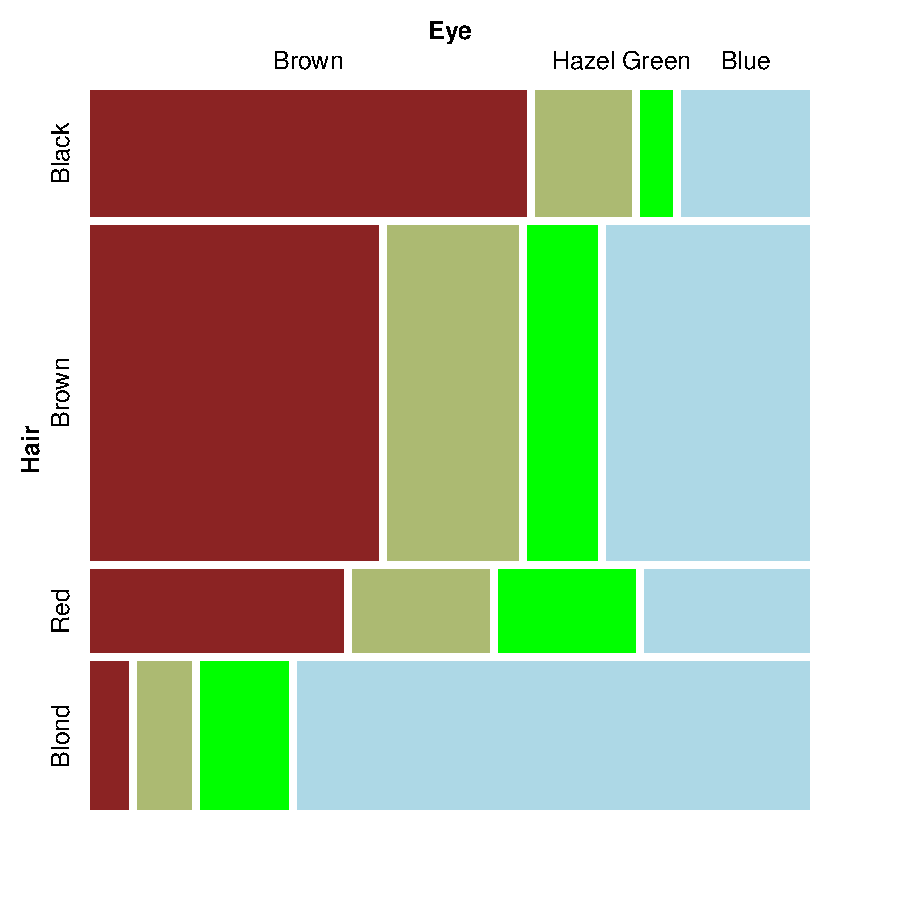
\includegraphics[width=.49\textwidth]{ch05/fig/HE-fill-1} 
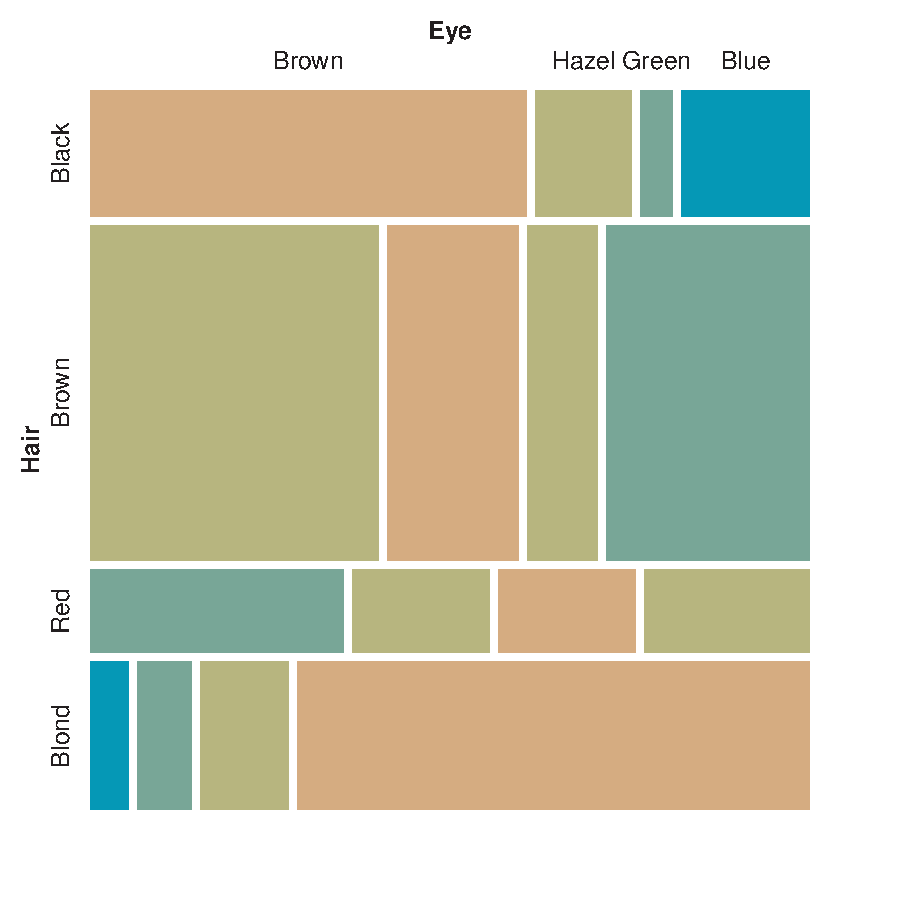
\includegraphics[width=.49\textwidth]{ch05/fig/HE-fill-2} }

\caption[Mosaic displays for the 	exttt{haireye2} data, using custom colors to fill the tiles]{Mosaic displays for the 	exttt{haireye2} data, using custom colors to fill the tiles. Left: Marimekko chart, using colors to reflect the eye colors; right: Toeplitz-based colors, reflecting the diagonal strips in a square table.\label{fig:HE-fill}}
\end{figure}


\end{knitrout}

%% \begin{figure}
%% \centering
%% 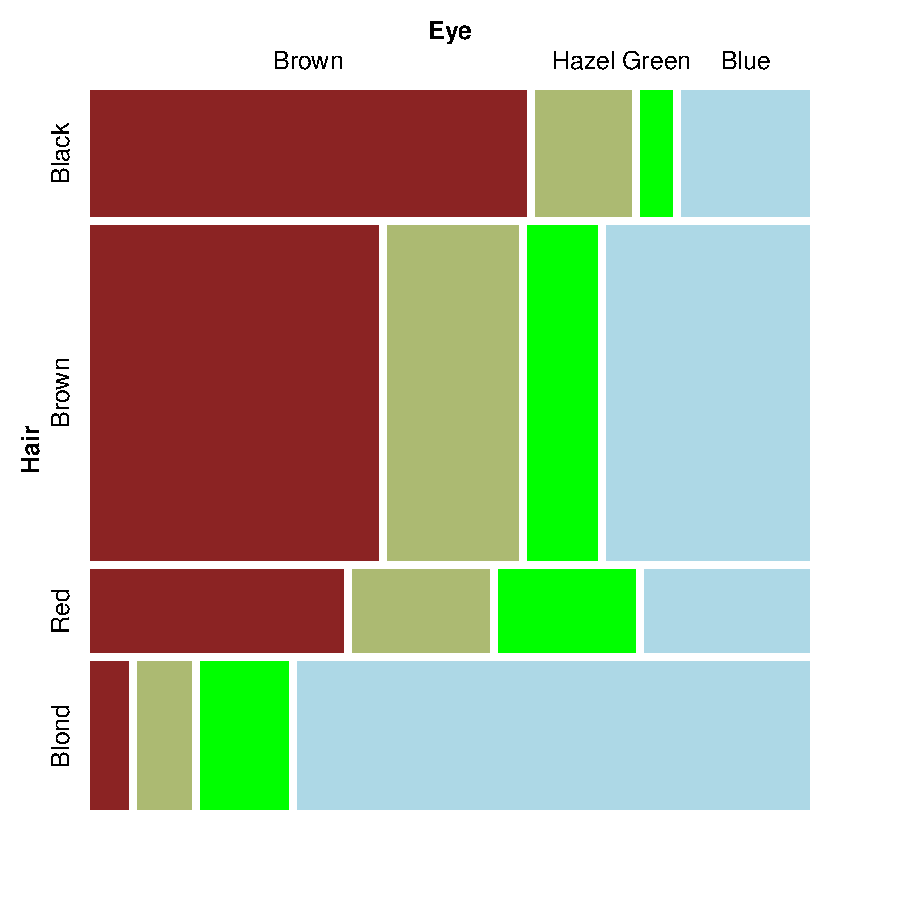
\includegraphics[width=.49\textwidth]{ch05/fig/HE-fill1}
%% 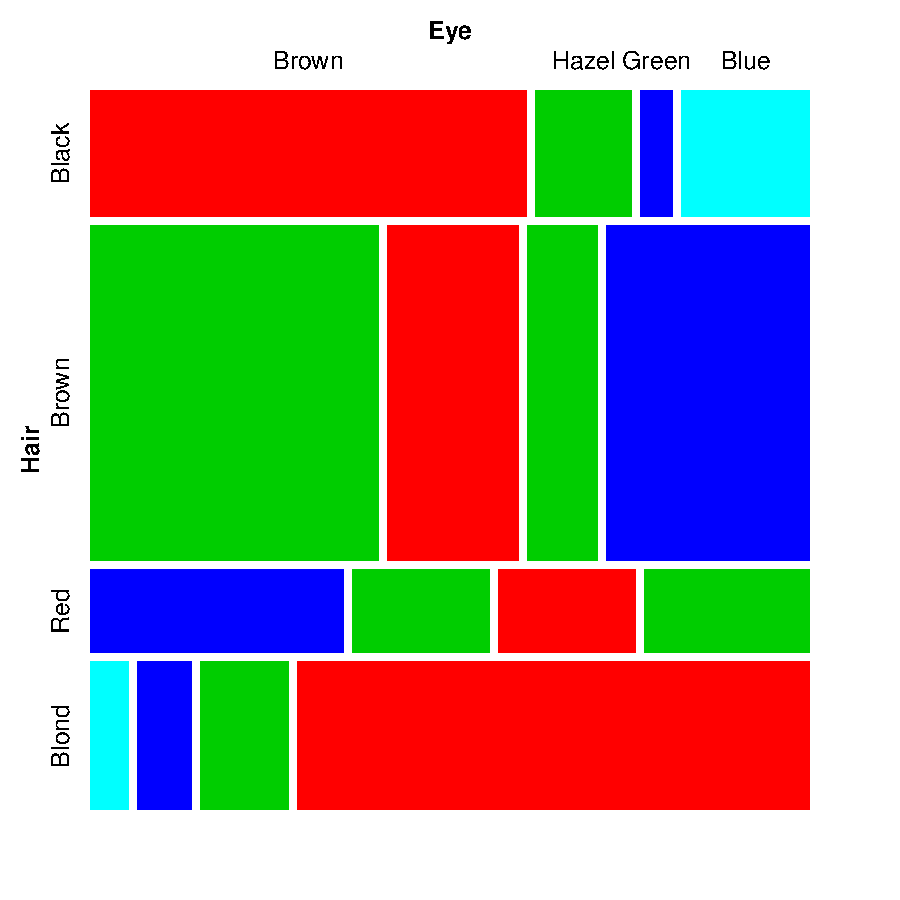
\includegraphics[width=.49\textwidth]{ch05/fig/HE-fill2}
%% \caption{Mosaic displays for the \texttt{haireye2} data, using custom colors to fill the tiles. Left: Marimekko chart, using colors to reflect the eye colors; right: Toeplitz-based colors, reflecting the diagonal strips in a square table.}\label{fig:HE-fill}
%% \end{figure}

More simply, to shade a mosaic according to the levels of one variable (typically a response variable),
you can use the \code{highlighting} arguments of \func{mosaic}.
The first call below gives a result similar to the left panel of \figref{fig:HE-fill}.
Alternatively, using the formula method for \func{mosaic}, specify the response
variable as the left-hand side.

\begin{knitrout}
\definecolor{shadecolor}{rgb}{1, 0.961, 0.933}\color{fgcolor}\begin{kframe}
\begin{alltt}
\hlstd{> }\hlkwd{mosaic}\hlstd{(haireye2,} \hlkwc{highlighting} \hlstd{=} \hlstr{"Eye"}\hlstd{,} \hlkwc{highlighting_fill} \hlstd{= fill_colors)}
\hlstd{> }\hlkwd{mosaic}\hlstd{(Eye} \hlopt{~} \hlstd{Hair,} \hlkwc{data} \hlstd{= haireye2,} \hlkwc{highlighting_fill} \hlstd{= fill_colors)}
\end{alltt}
\end{kframe}
\end{knitrout}


\subsubsection{Residual-based shading}
The important idea that differentiates mosaic and other strucplot displays from the
``poor-man's,'' Marimekko versions (\figref{fig:HE-fill})
often shown in other software is that rather than
just using shading color to \emph{identify} the cells, we can use these attributes to
show something more--- \emph{residuals} from some model, whose pattern helps to explain
the association between the table variables.

As described above, the strucplot framework includes a variety of \code{shading\_} functions,
and these can be customized with optional arguments.
\citet{Zeileis-etal:2007} describe a general approach to residual-based shadings for area-proportional
visualizations, used in the development of the strucplot framework in \pkg{vcd}.

\begin{Example}[interp]{Interpolation options}
One simple thing to do is to modify the \code{interpolate} option passed to the
default \code{shading\_hcl} function, as shown in \figref{fig:HE-interp}.
\begin{knitrout}
\definecolor{shadecolor}{rgb}{1, 0.961, 0.933}\color{fgcolor}\begin{kframe}
\begin{alltt}
\hlstd{> }\hlcom{# more shading levels}
\hlstd{> }\hlkwd{mosaic}\hlstd{(haireye2,} \hlkwc{shade} \hlstd{=} \hlnum{TRUE}\hlstd{,} \hlkwc{gp_args} \hlstd{=} \hlkwd{list}\hlstd{(}\hlkwc{interpolate} \hlstd{=} \hlnum{1} \hlopt{:} \hlnum{4}\hlstd{))}
\hlstd{> }
\hlstd{> }\hlcom{# continuous shading}
\hlstd{> }\hlstd{interp} \hlkwb{<-} \hlkwa{function}\hlstd{(}\hlkwc{x}\hlstd{)} \hlkwd{pmin}\hlstd{(x} \hlopt{/} \hlnum{6}\hlstd{,} \hlnum{1}\hlstd{)}
\hlstd{> }\hlkwd{mosaic}\hlstd{(haireye2,} \hlkwc{shade} \hlstd{=} \hlnum{TRUE}\hlstd{,} \hlkwc{gp_args} \hlstd{=} \hlkwd{list}\hlstd{(}\hlkwc{interpolate} \hlstd{= interp))}
\end{alltt}
\end{kframe}\begin{figure}[!htbp]

\centerline{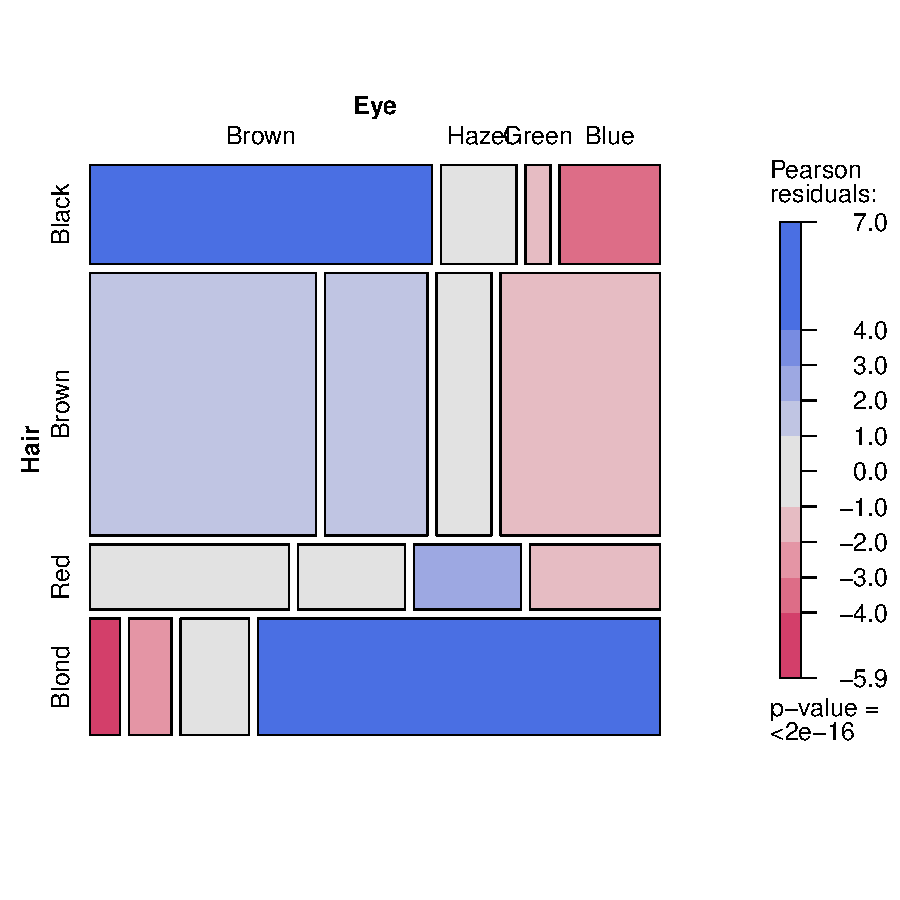
\includegraphics[width=.49\textwidth]{ch05/fig/HE-interp-1} 
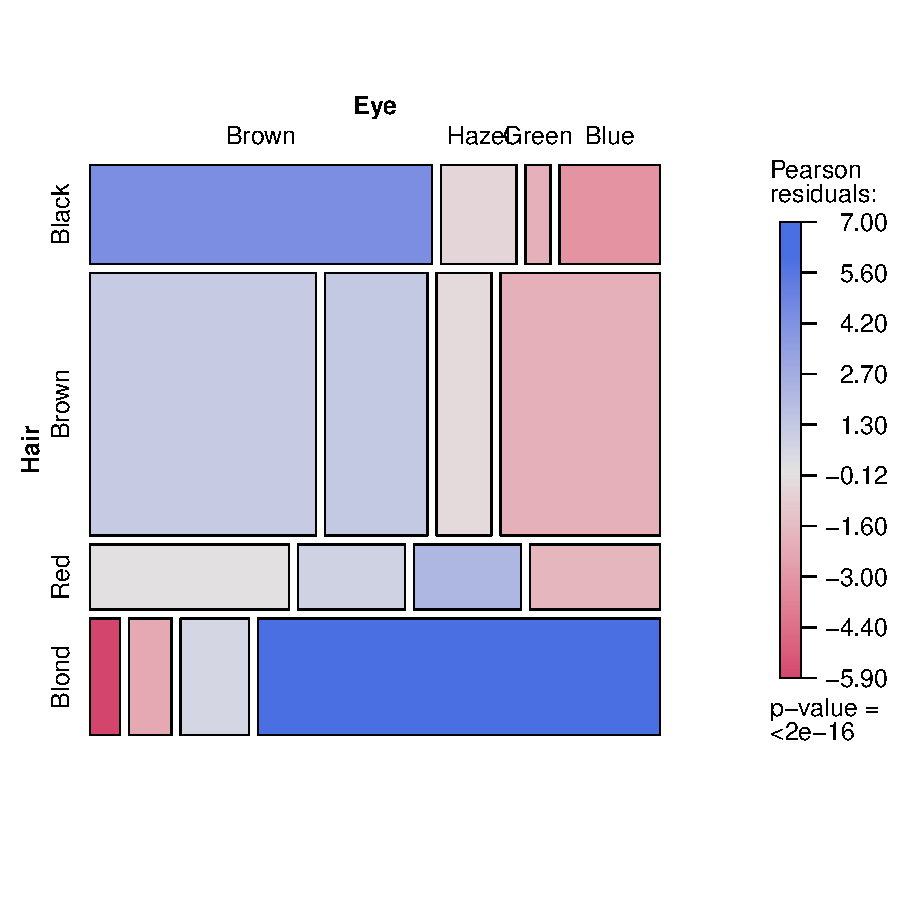
\includegraphics[width=.49\textwidth]{ch05/fig/HE-interp-2} }

\caption[Interpolation options for shading levels in mosaic displays]{Interpolation options for shading levels in mosaic displays. Left: four shading levels; right: continuous shading.\label{fig:HE-interp}}
\end{figure}


\end{knitrout}
For the left panel of \figref{fig:HE-interp}, a numeric vector is passed as \code{interpolate=1:4}, defining the
boundaries of a step function mapping the absolute values of residuals to
saturation levels in the HCL color scheme.
For the right panel, a user-defined function, \func{interp}, is created which maps
the absolute residuals to saturation values in a continuous way (up to a maximum of 6).

Note that these two interpolation schemes produce quite similar results, differing
mainly in the shading level of residuals within $\pm 1$ and in the legend.
In practice, the default discrete interpolation, using cutoffs of $\pm 2, \pm 4$
usually works quite well.
\end{Example}

\begin{Example}[shading]{Shading functions}
Alternatively, the names of shading functions can be passed as the \code{gp} argument,
as shown below, producing \figref{fig:HE-shading}.   Two shading function are illustrated
here:
\begin{itemize*}
  \item The left panel of \figref{fig:HE-shading} uses the classical \citet{Friendly:94a}
  shading scheme, \code{shading\_Friendly} with HSV colors of blue and red and
  default cutoffs for absolute residuals, $\pm 2, \pm 4$,
  corresponding to \code{interpolate = c(2, 4)}.  In this shading scheme,
  all tiles use an outline color (\code{col}) corresponding to the sign of the residual.
  As well, the border line type (\code{lty}) distinguishes positive and negative residuals,
  which is useful if a mosaic plot is printed in black and white.

\item The right panel uses the \func{shading\_max} function, based on the ideas of
   \citet{Zeileis-etal:2007} on residual-based shadings for area-proportional
   visualizations.
   Instead of using the cut-offs 2 and 4, it employs the critical values, $M_\alpha$,
   for the maximum
   absolute Pearson residual statistic,
%   $M = \max_{i, j} | r_{ij} |$,
\begin{equation*} \label{eq:MaxAbs}
M \quad = \quad \max_{i, j} |r_{ij}| \comma
\end{equation*}
by default at $\alpha =$ 0.10 and 0.01.%
\footnote{
These default significance levels were chosen because this
leads to displays where fully colored cells are clearly significant ($p < 0.01$),
cells without color are clearly non-significant ($p > 0.1$), and
cells in between can be considered to be weakly significant ($0.01 \le p \le 0.1$).
}
   Only those residuals with $| r_{ij} | >  M_\alpha$ are colored in the plot,
   using two levels for Value (``lightness'') in HSV color space.
   Consequently, all
   color in the plot signals a significant departure from independence
   at 90\% or 99\% significance level, respectively.%
\footnote{
This computation uses the \pkg{vcd} function \func{coindep\_test}
to calculate generalized tests of (conditional) independence
by simulation from the marginal distribution of the input table under (conditional) independence.
In these examples using \code{shading\_max}, the function \func{set.seed} is used to
initialize the random number generators to a given state for reproducibility.
}
\end{itemize*}

\begin{knitrout}
\definecolor{shadecolor}{rgb}{1, 0.961, 0.933}\color{fgcolor}\begin{kframe}
\begin{alltt}
\hlstd{> }\hlkwd{mosaic}\hlstd{(haireye2,} \hlkwc{gp} \hlstd{= shading_Friendly,} \hlkwc{legend} \hlstd{= legend_fixed)}
\hlstd{> }\hlkwd{set.seed}\hlstd{(}\hlnum{1234}\hlstd{)}
\hlstd{> }\hlkwd{mosaic}\hlstd{(haireye2,} \hlkwc{gp} \hlstd{= shading_max)}
\end{alltt}
\end{kframe}\begin{figure}[!htbp]

\centerline{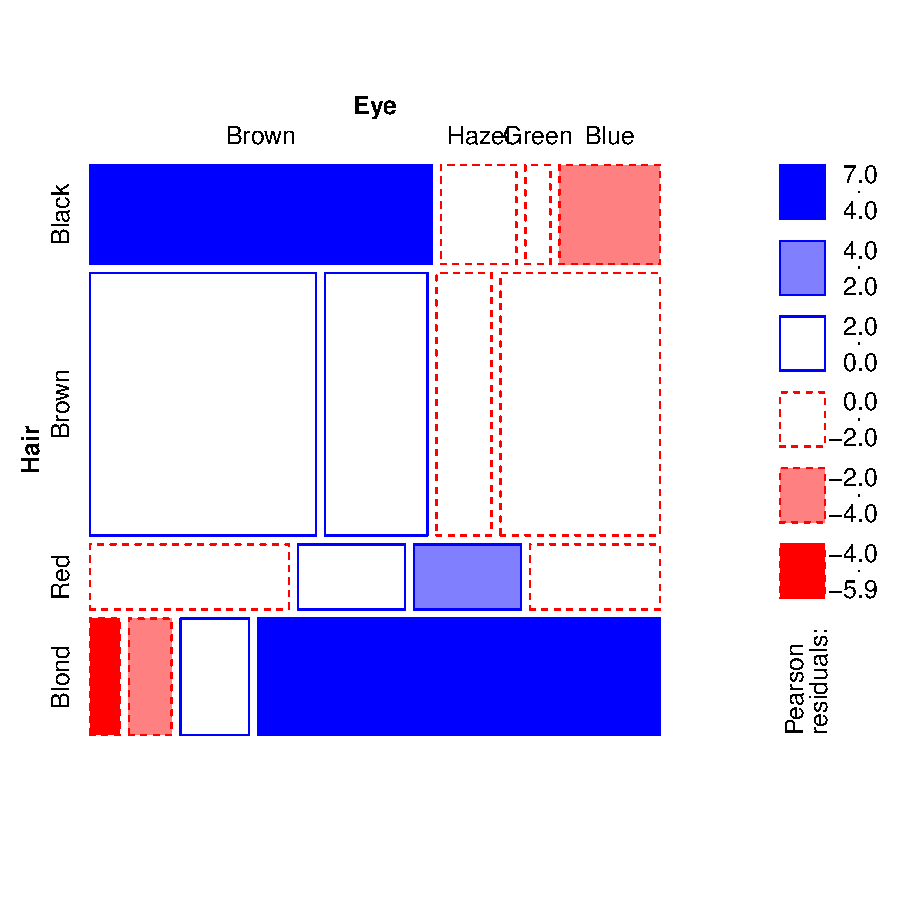
\includegraphics[width=.49\textwidth]{ch05/fig/HE-shading-1} 
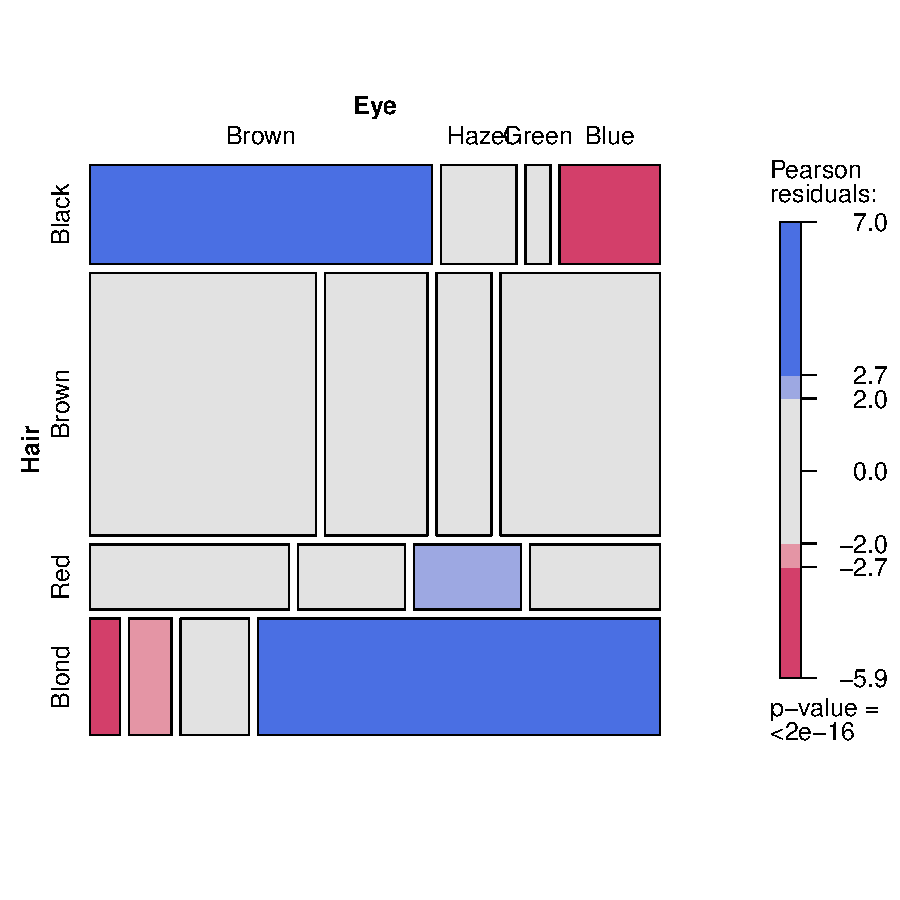
\includegraphics[width=.49\textwidth]{ch05/fig/HE-shading-2} }

\caption{Shading functions for mosaic displays. Left: \code{shading\_Friendly} using fixed cutoffs and the ``Friendly'' color scheme; right: \code{shading\_max}, using a permutation-based test to determine significance of residuals.\label{fig:HE-shading}}
\end{figure}


\end{knitrout}
In this example, the difference between these two shading schemes is largely cosmetic, in that
the pattern of association is similar in the two panels of \figref{fig:HE-shading}, and the
interpretation would be the same.  This is not always the case, as we will see in the
next example.
\end{Example}

\begin{Example}[arth-mosaic]{Arthritis treatment}

This example uses the \data{Arthritis} data, illustrated earlier (\exref{ex:ch2-arth}),
on the relation between treatment and outcome for rheumatoid arthritis.
To confine this example to a two-way table, we use only the (larger) female
patient group.
\begin{knitrout}
\definecolor{shadecolor}{rgb}{1, 0.961, 0.933}\color{fgcolor}\begin{kframe}
\begin{alltt}
\hlstd{> }\hlstd{art} \hlkwb{<-} \hlkwd{xtabs}\hlstd{(}\hlopt{~} \hlstd{Treatment} \hlopt{+} \hlstd{Improved,} \hlkwc{data} \hlstd{= Arthritis,}
\hlstd{+ }             \hlkwc{subset} \hlstd{= Sex} \hlopt{==} \hlstr{"Female"}\hlstd{)}
\hlstd{> }\hlkwd{names}\hlstd{(}\hlkwd{dimnames}\hlstd{(art))[}\hlnum{2}\hlstd{]} \hlkwb{<-} \hlstr{"Improvement"}
\end{alltt}
\end{kframe}
\end{knitrout}
The calls to \func{mosaic} below compare \code{shading\_Friendly} and \code{shading\_max},
giving the plots shown in \figref{fig:arth-mosaic}.

\begin{knitrout}
\definecolor{shadecolor}{rgb}{1, 0.961, 0.933}\color{fgcolor}\begin{kframe}
\begin{alltt}
\hlstd{> }\hlkwd{mosaic}\hlstd{(art,} \hlkwc{gp} \hlstd{= shading_Friendly,} \hlkwc{margin} \hlstd{=} \hlkwd{c}\hlstd{(}\hlkwc{right} \hlstd{=} \hlnum{1}\hlstd{),}
\hlstd{+ }       \hlkwc{labeling} \hlstd{= labeling_residuals,} \hlkwc{suppress} \hlstd{=} \hlnum{0}\hlstd{,} \hlkwc{digits} \hlstd{=} \hlnum{2}\hlstd{)}
\hlstd{> }\hlkwd{set.seed}\hlstd{(}\hlnum{1234}\hlstd{)}
\hlstd{> }\hlkwd{mosaic}\hlstd{(art,} \hlkwc{gp} \hlstd{= shading_max,} \hlkwc{margin} \hlstd{=} \hlkwd{c}\hlstd{(}\hlkwc{right} \hlstd{=} \hlnum{1}\hlstd{))}
\end{alltt}
\end{kframe}\begin{figure}[!htbp]

\centerline{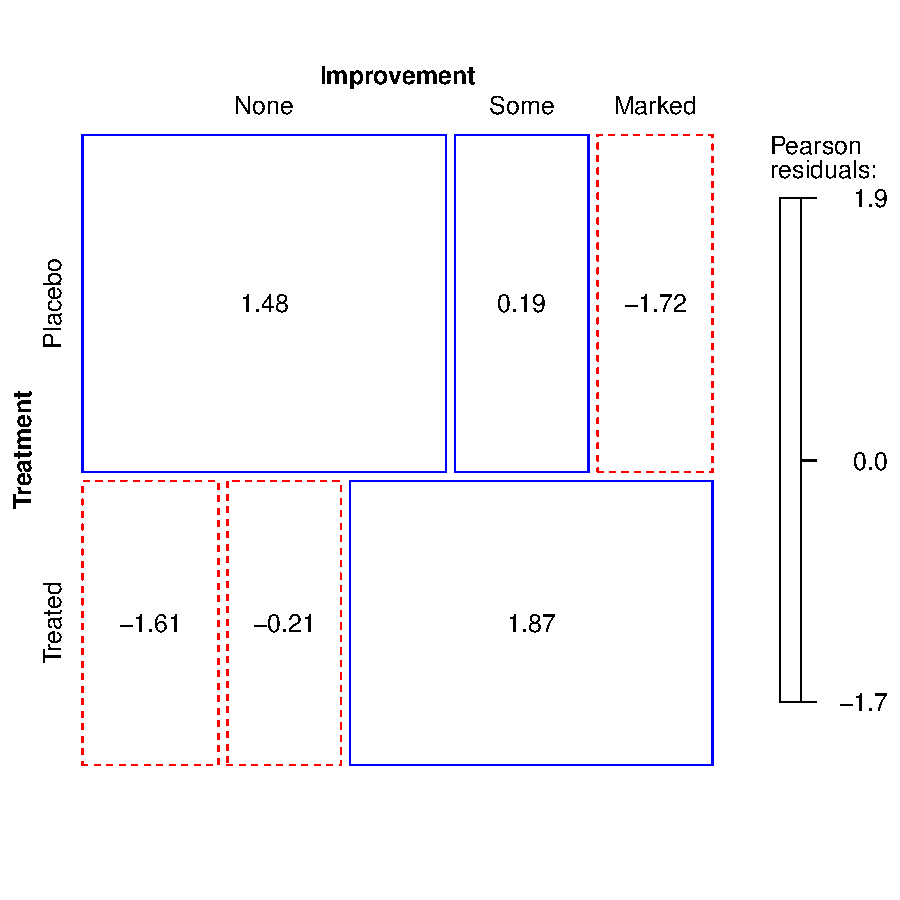
\includegraphics[width=.49\textwidth]{ch05/fig/arth-mosaic-1} 
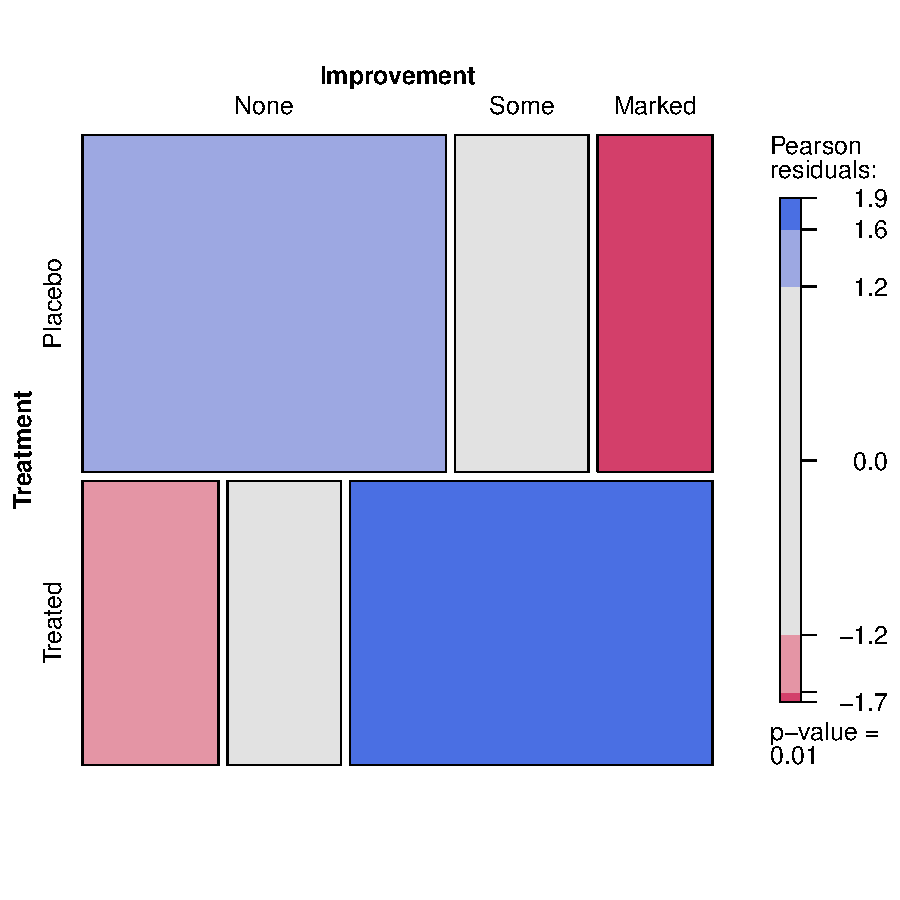
\includegraphics[width=.49\textwidth]{ch05/fig/arth-mosaic-2} }

\caption{Mosaic plots for the female patients in the \code{Arthritis} data. Left: Fixed shading levels via \code{shading\_Friendly}; right: shading levels determined by significant maximum residuals via \code{shading\_max}.\label{fig:arth-mosaic}}
\end{figure}


\end{knitrout}
This data set is somewhat paradoxical, in that the standard \func{chisq.test} for
association with these data gives a highly significant result,
$\chi^2 (2) = 11.3, p = 0.0035$, while the shading pattern using
\code{shading\_Friendly} in the left panel of \figref{fig:arth-mosaic}
shows all residuals within $\pm 2$, and thus unshaded.

On the other hand, the \code{shading\_max} shading in the right panel of \figref{fig:arth-mosaic}
shows that significant deviations from independence occur in the four corner cells, corresponding
to more of the treated group showing marked improvement, and more of the placebo group showing
no improvement.

Some details behind the \code{shading\_max} method are shown below.  The Pearson residuals
for this table are calculated as:
\begin{knitrout}
\definecolor{shadecolor}{rgb}{1, 0.961, 0.933}\color{fgcolor}\begin{kframe}
\begin{alltt}
\hlstd{> }\hlkwd{residuals}\hlstd{(}\hlkwd{chisq.test}\hlstd{(art))}
\end{alltt}
\begin{verbatim}
         Improvement
Treatment     None     Some   Marked
  Placebo  1.47752  0.19267 -1.71734
  Treated -1.60852 -0.20975  1.86960
\end{verbatim}
\end{kframe}
\end{knitrout}
The \func{shading\_max} function then calls \code{coindep\_test(art)} to generate
$n=1000$ random tables with the same margins, and computes the maximum residual statistic
for each.  This gives a non-parametric $p$-value for the test of independence,
$p =0.011$
% art_max$p.value
shown in the legend.
\begin{knitrout}
\definecolor{shadecolor}{rgb}{1, 0.961, 0.933}\color{fgcolor}\begin{kframe}
\begin{alltt}
\hlstd{> }\hlkwd{set.seed}\hlstd{(}\hlnum{1243}\hlstd{)}
\hlstd{> }\hlstd{art_max} \hlkwb{<-} \hlkwd{coindep_test}\hlstd{(art)}
\hlstd{> }\hlstd{art_max}
\end{alltt}
\begin{verbatim}

	Permutation test for conditional independence

data:  art
f(x) = 1.8696, p-value = 0.011
\end{verbatim}
\end{kframe}
\end{knitrout}
Finally, the 0.90 and 0.99 quantiles of the simulation distribution are used as
shading levels, passed as the value of the \code{interpolate} argument.
\begin{knitrout}
\definecolor{shadecolor}{rgb}{1, 0.961, 0.933}\color{fgcolor}\begin{kframe}
\begin{alltt}
\hlstd{> }\hlstd{art_max}\hlopt{$}\hlkwd{qdist}\hlstd{(}\hlkwd{c}\hlstd{(}\hlnum{0.90}\hlstd{,} \hlnum{0.99}\hlstd{))}
\end{alltt}
\begin{verbatim}
   90%    99% 
1.2393 1.9167 
\end{verbatim}
\end{kframe}
\end{knitrout}
\end{Example}

The converse situation can also arise in practice. An overall test for association
using Pearson's $\chi^2$ may not be significant, but the maximum residual test
may highlight one or more cells worthy of greater attention, as illustrated in
the following example.


\begin{Example}[soccer2]{UK Soccer scores}
In \exref{ex:soccer}, we examined the distribution of goals scored
by the home team and the away team in 380 games in the 1995/96 season
by the 20 teams in the UK Football Association, Premier League.
The analysis there focused on the distribution of the total goals
scored, under the assumption that the number of goals scored by
the home team and the away team were independent.

Here, the rows and columns of the table \data{UKSoccer} are both ordered,
so it is convenient and compact to carry out all the CMH tests taking
ordinality into account.
\begin{knitrout}
\definecolor{shadecolor}{rgb}{1, 0.961, 0.933}\color{fgcolor}\begin{kframe}
\begin{alltt}
\hlstd{> }\hlkwd{data}\hlstd{(}\hlstr{"UKSoccer"}\hlstd{,} \hlkwc{package} \hlstd{=} \hlstr{"vcd"}\hlstd{)}
\hlstd{> }\hlkwd{CMHtest}\hlstd{(UKSoccer)}
\end{alltt}
\begin{verbatim}
Cochran-Mantel-Haenszel Statistics for Home by Away 

                 AltHypothesis Chisq Df  Prob
cor        Nonzero correlation  1.01  1 0.315
cmeans  Col mean scores differ  5.63  4 0.229
rmeans  Row mean scores differ  7.42  4 0.115
general    General association 18.65 16 0.287
\end{verbatim}
\end{kframe}
\end{knitrout}
All of these are non-significant, so that might well be the end of the story,
as far as independence of goals in home and away games is concerned. Yet, one
residual, $r_{42} = 3.08$ stands out, corresponding to 4 or more goals by
the home team and only 2 goals by the away team, which accounts for nearly
half of the $\chi^2 (16) = 18.7$ for general association.

\begin{knitrout}
\definecolor{shadecolor}{rgb}{1, 0.961, 0.933}\color{fgcolor}\begin{kframe}
\begin{alltt}
\hlstd{> }\hlkwd{set.seed}\hlstd{(}\hlnum{1234}\hlstd{)}
\hlstd{> }\hlkwd{mosaic}\hlstd{(UKSoccer,} \hlkwc{gp} \hlstd{= shading_max,} \hlkwc{labeling} \hlstd{= labeling_residuals,} \hlkwc{digits} \hlstd{=} \hlnum{2}\hlstd{)}
\end{alltt}
\end{kframe}\begin{figure}[!htbp]

\centerline{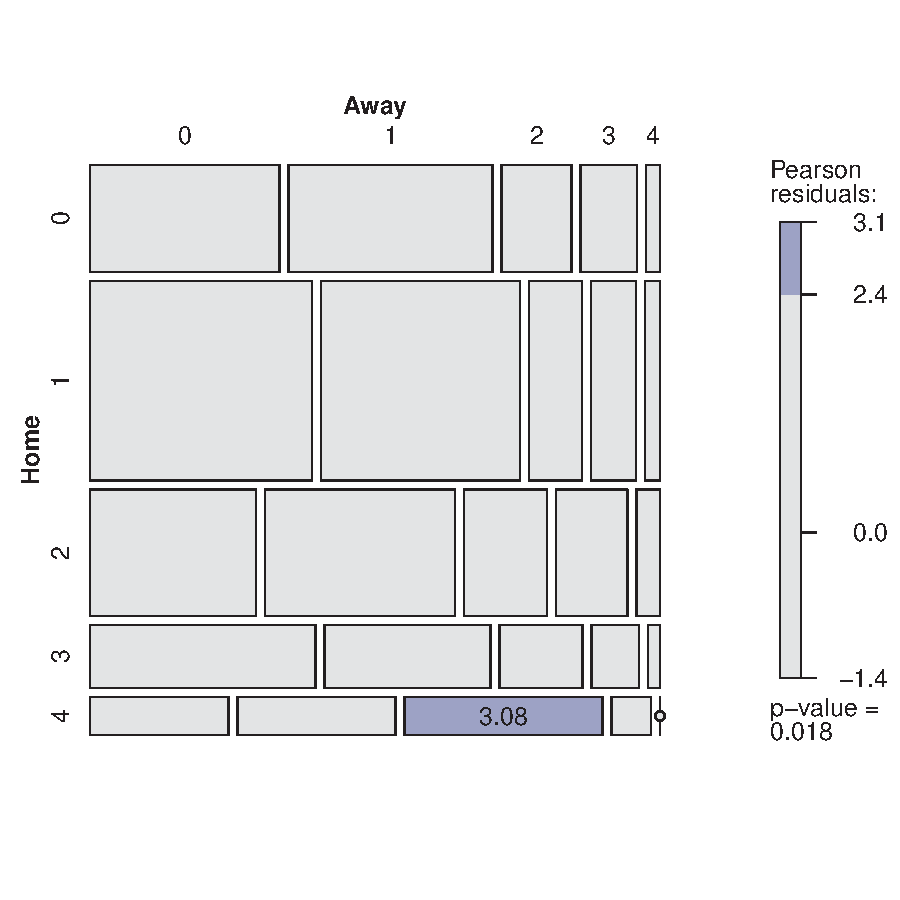
\includegraphics[width=.6\textwidth]{ch05/fig/UKsoccer-mosaic-1} }

\caption[Mosaic display for UK soccer scores, highlighting one cell that stands out for further attention]{Mosaic display for UK soccer scores, highlighting one cell that stands out for further attention\label{fig:UKsoccer-mosaic}}
\end{figure}


\end{knitrout}
This occurrence may or may not turn out to have some explanation, but at least
the mosaic plot draws it to our attention, and is consistent with the
(significant) result from \func{coindep\_test}.
%\TODO{Complete this example}
\end{Example}



\section{Three-way and larger tables}\label{sec:mosaic-threeway}


The mosaic displays and other graphical methods within the strucplot framework
extend quite naturally to three-way and higher-way tables.
The essential idea is that for the variables in a \mway table in a given order,
each successive variable is used to subdivide the tile(s) in proportion to
the relative (conditional) frequencies of that variable, given all previous
variables.  This process continues recursively until all table variables
have been included.

For simplicity, we continue with the running example of Hair color and Eye color.
Imagine that each
cell of the two-way table for Hair and Eye color is further
classified by one or more additional variables---sex and level of
education, for example.  Then each rectangle can be subdivided
horizontally to show the proportion of males and females in that
cell, and each of those horizontal portions can be subdivided
vertically to show the proportions of people at each educational
level in the hair-eye-sex group.

\begin{Example}[HEC1]{Hair color, eye color and sex}
\figref{fig:HEC-mos1} shows the mosaic for the three-way table, with Hair and Eye color
groups divided according to the proportions of Males and Females.
As explained in the next section (\secref{sec:mosaic-fitting})
there are different models for
``independence'' we could display.  Here, we show residuals for
the model of joint independence, \LLM{HairEye,Sex}, which
asserts that the combinations of Hair color and Eye color are
independent of Sex.  This model, and the corresponding mosaic
plot does \emph{not} show the (overall) association between Hair color
and Eye color we explored in earlier examples (see \figref{fig:haireye-mos8}).  It merely shows how where the Hair color--Eye color
combinations might differ by Sex.

In the call to \func{mosaic} below, the model of joint independence
is specified as the argument \verb|expected = ~ Hair*Eye + Sex|.
The strucplot labeling function \code{labeling\_residuals}
is used to display the residuals in the highlighted cells.
\begin{knitrout}
\definecolor{shadecolor}{rgb}{1, 0.961, 0.933}\color{fgcolor}\begin{kframe}
\begin{alltt}
\hlstd{> }\hlstd{HEC} \hlkwb{<-} \hlstd{HairEyeColor[,} \hlkwd{c}\hlstd{(}\hlstr{"Brown"}\hlstd{,} \hlstr{"Hazel"}\hlstd{,} \hlstr{"Green"}\hlstd{,} \hlstr{"Blue"}\hlstd{),]}
\hlstd{> }\hlkwd{mosaic}\hlstd{(HEC,} \hlkwc{expected} \hlstd{=} \hlopt{~} \hlstd{Hair} \hlopt{*} \hlstd{Eye} \hlopt{+} \hlstd{Sex,}
\hlstd{+ }       \hlkwc{labeling} \hlstd{= labeling_residuals,} \hlkwc{digits} \hlstd{=} \hlnum{2}\hlstd{)}
\end{alltt}
\end{kframe}\begin{figure}[!htb]

\centerline{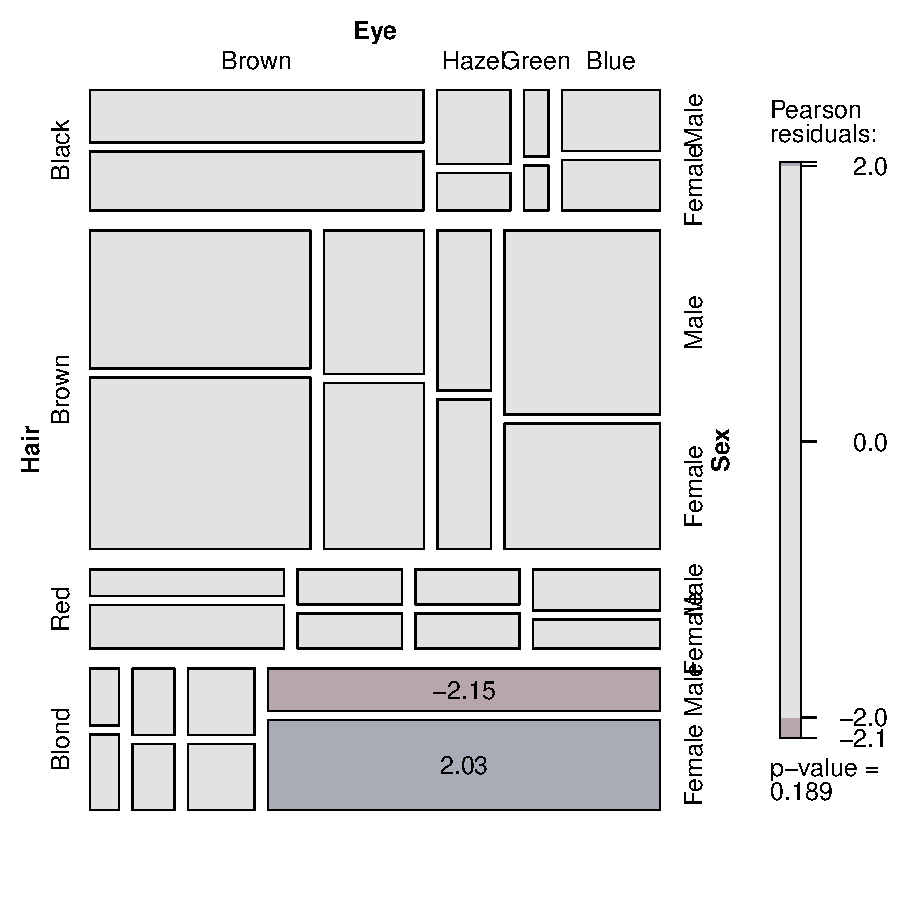
\includegraphics[width=.7\textwidth]{ch05/fig/HEC-mos1-1} }

\caption[Three-way mosaic for Hair color, Eye color and Sex]{Three-way mosaic for Hair color, Eye color and Sex. Residuals from the model of joint independence, [HE][S] are shown by shading.\label{fig:HEC-mos1}}
\end{figure}


\end{knitrout}
In \figref{fig:HEC-mos1} it is easy to
see that there is no systematic association between sex
and the combinations of Hair and Eye color---except among
blue-eyed blonds, where there are an overabundance of females.

The model of joint independence has a non-significant Pearson
$\chi^2 (15) = 19.567, p=0.189$. Yet, the two largest residuals
highlighted in the plot account for nearly half
($-2.15^2 + 2.03^2 = 8.74$) of the lack of fit, and so are worthy
of attention here.  An easy (probably facile) interpretation is
that among the blue-eyed blonds, some of the females benefited from
hair products.
\end{Example}

\subsection{Fitting models}\label{sec:mosaic-fitting}
When three or more variables are
represented in a table, we can fit several different models of types of
``independence'' and display the residuals from each model.  We treat
these models as null or \term{baseline models}, which may not fit the data
particularly well.  The deviations of observed frequencies from
expected ones, displayed by shading, will often suggest terms to be added
to an explanatory model that achieves a better fit.

For a three-way table, with variables $A$, $B$ and $C$, some of the hypothesized models which can be fit are
described below and summarized in \tabref{tab:hyp3way}.
Here we use $[\bullet]$ notation to list the \term{high-order terms} in
a hierarchical \loglin model; these correspond to the margins
of the table which are fitted exactly, and which translate
directly into \R formulas used in \func{loglm} and
\code{mosaic(..., expected=)}.
\TODO{Tweak the association diagrams here to use smaller circles, allowing longer connecting lines.}

The notation \LLM{AB,AC},
for example, is shorthand for the model \verb|loglm(~ A*B + A*C)| that implies
\begin{equation} \label{eq:AB-AC}
  \log \,  m_{ijk}  =
  \mu  +  \lambda_i^A
  +  \lambda_j^B
  +  \lambda_k^C
  +  \lambda_{ij}^{AB}
  +  \lambda_{ik}^{AC}
  \comma
\end{equation}
(as described in \secref{sec:loglin-counts}) and reproduces the
$\{AB\}$ and $\{AC\}$ marginal subtables.%
\footnote{
The notation here uses curly braces, $\{\bullet\}$ to indicate a marginal
subtable summed over all other variables.
}
That is, the calculated
expected frequencies in these margins are always equal to the
corresponding observed frequencies,
$m_{ij+} = n_{ij+}$ and
$m_{i+k} = n_{i+k}$.

\begin{comment}
\newcommand{\tridot}[1]{%
	\begin{pspicture}(-.01, -.01)(1.1,1.1)%
	\psset{xunit=.85cm,yunit=.85cm}%
	\color{black}%
	\rput(0,0){\circlenode{A}{\textsf{A}}}%
	\rput(1.0,0){\circlenode{B}{\textsf{B}}}%
	\rput(.5,.866){\circlenode{C}{\textsf{C}}}%
	#1%
	\end{pspicture}%
	\rule{0in}{1.2cm}
%	}
}
\end{comment}

\newcommand{\tridot}[1]{%
\begin{tikzpicture}[x=0.9cm, y=0.9cm]
  \node(A)[draw, circle, fill=yellow!30,scale=0.9] at (0,0) {\textbf{\textsf{A}}};
  \node(B)[draw, circle, fill=yellow!30,scale=0.9] at (1,0) {\textbf{\textsf{B}}};
  \node(C)[draw, circle, fill=yellow!30,scale=0.9] at (.5,.866) {\textbf{\textsf{C}}};
  #1%
%  \path (A) edge (B);
%  \path (B) edge (C);
%  \draw (0,0) circle 
\end{tikzpicture}
}


\begin{table}[htb]
\caption[Hypotheses for a three-way table]{Fitted margins, model symbols and interpretations for some hypotheses for a three-way table.}\label{tab:hyp3way}
\begin{center}
  \begin{tabular}{|clllc|} \hline
  \tableheader
  Hypothesis & \multilineC{Fitted\\margins} & \multilineC{Model\\symbol} & \multilineC{Independence\\interpretation} & \multilineC{Association\\graph} \\
%             & Fitted  & Model &  Independence  & Association  \\
%  Hypothesis & margins & symbol & Interpretation & graph \\
   \hline 
  $H_1$ & $n_{i++}, n_{+j+}, n_{++k}$ & [A][B][C] & $A \perp B \perp C $ & 
  \tridot{} \\[3ex] 
  $H_2$ & $n_{ij+}, n_{++k}$ & [AB][C] & $(A , B )\perp C $ & 
  \tridot{\path (A) edge (B);} \\[3ex]
%
  $H_3$ & $n_{i+k}, n_{+jk}$ & [AC][BC] & $A \perp B \: |\: C$ & 
  \tridot{\path (A) edge (C); \path (B) edge (C);} \\[3ex]
  $H_4$ & $n_{ij+}, n_{i+k}, n_{+jk}$ & [AB][AC][BC] & \texttt{NA} & 
  \tridot{\path (A) edge (B); \path (B) edge (C); \path (A) edge (C);} \\[3ex]
%
  \hline
  \end{tabular}
 \end{center}
\end{table}


In this table, $A \perp B$ is
read, ``$A$ is independent of $B$.'' The independence interpretation
of the model \eqref{eq:AB-AC} is $B \perp C \given A$,
which can be read as ``$B$ is independent of $C$, given (conditional on) $A$.''
\tabref{tab:hyp3way} also
depicts the relations among variables as an
\term{association graph}, where associated variables are connected by an edge
and variables that are asserted to be independent are unconnected.
In mosaic-like displays,
other associations present in the data will appear in the pattern of
residuals.

For a three-way table, there are four general classes of independence models
illustrated in \tabref{tab:hyp3way}, as described below.%
\footnote{For $H_2$ and $H_3$, permutation of the variables A, B, and C gives
other members of each class.}
Not included here
is the \term{saturated model}, \LLM{ABC}, which fits the observed data
exactly.

\begin{description}
\item[$H_1$: Complete independence.]  The model of complete (mutual) independence, symbolized $A \perp B \perp C$, with model formula \verb|~ A + B + C|,
       asserts that all joint probabilities are products of the
       one-way marginal probabilities:
\begin{equation*}
 \pi_{ijk} = \pi_{i++} \: \pi_{+j+} \: \pi_{++k}
 \comma
\end{equation*}
for all \(i , j , k\) in a
       three-way table.  This corresponds to the log-linear model
       \LLM{A,B,C}.  Fitting this model puts all higher
       terms, and hence all association among the variables, into the
       residuals.

\item[$H_2$: Joint independence.]  Another possibility is to fit the model in
       which variable \(C\) is jointly independent of variables \(A\)
       and \(B\), (\{$A , B \} \perp C $), with model formula \verb|~ A*B + C|,
       where
\begin{equation*}
 \pi_{ijk}  =  \pi_{ij+} \:  \pi_{++k} \period
\end{equation*}
This corresponds to the \loglin model \LLM{AB,C}.
Residuals from this model show the extent to which
variable \(C\) is related to the combinations of variables
\(A\) and \(B\) but they do not show any association between
\(A\) and \(B\), since that association is fitted exactly.
For this model, variable $C$ is also independent of $A$ and
$B$ in the marginal $\{AC\}$ table (collapsing over $B$) and
in the marginal $\{BC\}$.

\item[$H_3$: Conditional independence.] Two variables, say $A$ and $B$ are conditionally independent
given the third ($C$) if $A$ and $B$ are independent when we
control for $C$, symbolized as $A \perp B \given C$, and model formula \verb|~ A*C + B*C|.
This means that conditional probabilities, $\pi_{ij|k}$ obey
\begin{equation*}
 \pi_{ij|k}  =  \pi_{i+|k} \:  \pi_{+j|k} \comma
\end{equation*}
where
$\pi_{ij|k} = \pi_{ijk} / \pi_{ij+}$,
$\pi_{i+|k} = \pi_{i+k} / \pi_{i++}$, and
$\pi_{+j|k} = \pi_{+jk} / \pi_{+j+}$.
The corresponding \loglin{} models is denoted \LLM{AC,BC}.
When this model is fit, the mosaic display shows the conditional
associations between variables $A$ and $B$, controlling for $C$,
but does not show the associations between $A$ and $C$, or
$B$ and $C$.

\item[$H_4$: No three-way interaction.]  For this model, no pair is
marginally or
conditionally independent, so there is \emph{no} independence interpretation.
Nor is there a closed-form expression for the cell probabilities.
However, the association between any two
variables is the same at each level of the third variable.
The corresponding \loglin model formula is \LLM{AB,AC,BC},
indicating that all two-way margins are fit exactly and so
only the three-way association is
shown in the mosaic residuals.
\end{description}

\TODO{Add a textbox or text describing the general scheme for translating
among \loglin shorthand, \R model formulas and independence interpretations.}

\begin{Example}[HEC2]{Hair color, eye color and sex}
We continue with the analysis of the \data{HairEyeColor} data from
\exref{ex:HEC1}.  \figref{fig:HEC-mos1} showed the fit of the
joint-independence model [HairEye][Sex], testing whether
the joint distribution of hair color and eye color is
associated with sex.

Any other model fit to this table will have the same size tiles in the mosaic
since the areas depend on the observed frequencies;  the residuals,
and hence the shading of the tiles will differ.  \figref{fig:HEC-mos2}
shows mosaics for two other models. Shading in the left panel shows
residuals from the model of mutual independence, [Hair][Eye][Sex], and so
includes all sources of association among these three variables.
The right panel shows the
conditional independence model, [HairSex][EyeSex]
testing whether, given sex, hair color and eye color are independent.
Note that the pattern of residuals here is
similar to that in the two-way display,
\figref{fig:haireye-mos9}, that collapsed over sex.

\begin{knitrout}
\definecolor{shadecolor}{rgb}{1, 0.961, 0.933}\color{fgcolor}\begin{kframe}
\begin{alltt}
\hlstd{> }\hlstd{abbrev} \hlkwb{<-} \hlkwd{list}\hlstd{(}\hlkwc{abbreviate}\hlstd{=}\hlkwd{c}\hlstd{(}\hlnum{FALSE}\hlstd{,} \hlnum{FALSE}\hlstd{,} \hlnum{1}\hlstd{))}
\hlstd{> }\hlkwd{mosaic}\hlstd{(HEC,} \hlkwc{expected} \hlstd{=} \hlopt{~} \hlstd{Hair} \hlopt{+} \hlstd{Eye} \hlopt{+} \hlstd{Sex,} \hlkwc{labeling_args} \hlstd{= abbrev,}
\hlstd{+ }  \hlkwc{main} \hlstd{=} \hlstr{"Model: ~ Hair + Eye + Sex"}\hlstd{)}
\hlstd{> }\hlkwd{mosaic}\hlstd{(HEC,} \hlkwc{expected} \hlstd{=} \hlopt{~} \hlstd{Hair} \hlopt{*} \hlstd{Sex} \hlopt{+} \hlstd{Eye} \hlopt{*} \hlstd{Sex,} \hlkwc{labeling_args} \hlstd{= abbrev,}
\hlstd{+ }        \hlkwc{main}\hlstd{=}\hlstr{"Model: ~ Hair*Sex + Eye*Sex"}\hlstd{)}
\end{alltt}
\end{kframe}\begin{figure}[!htbp]

\centerline{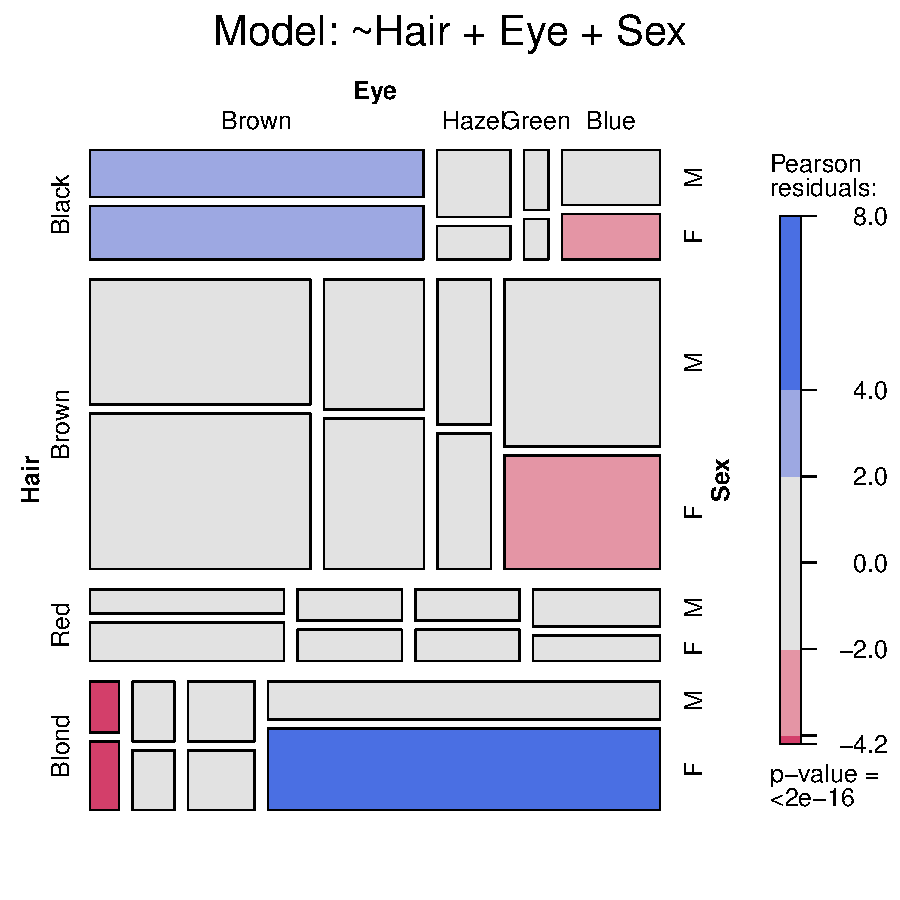
\includegraphics[width=.49\textwidth]{ch05/fig/HEC-mos2-1} 
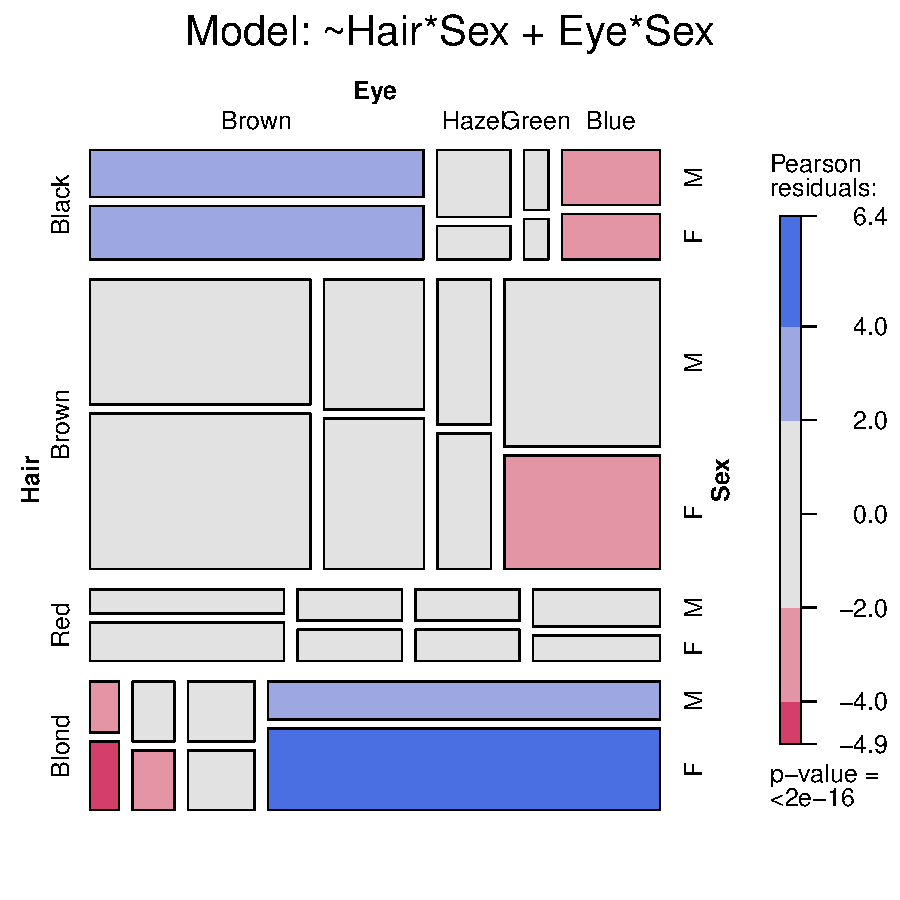
\includegraphics[width=.49\textwidth]{ch05/fig/HEC-mos2-2} }

\caption[Mosaic displays for other models fit to the data on Hair Color, Eye color and Sex]{Mosaic displays for other models fit to the data on Hair Color, Eye color and Sex.  Left: Mutual independence model; right: Conditional independence of Hair color and Eye color given Sex.\label{fig:HEC-mos2}}
\end{figure}


\end{knitrout}
\noindent Compared with \figref{fig:HEC-mos1} for the joint independence model, [HairEye][Sex],
it is easy to see that both of these models fit very poorly.

We consider \loglin models in more detail in \chref{ch:loglin}, but for now
note that these models are fit using \func{loglm} in the \Rpackage{MASS},
with the model formula given in the \argument{expected}.  The details of these
models can be seen by fitting these models explicitly, and the fit of
several models can be summarized compactly using \func{LRstats}
in \pkg{vcdExtra}.

\begin{knitrout}
\definecolor{shadecolor}{rgb}{1, 0.961, 0.933}\color{fgcolor}\begin{kframe}
\begin{alltt}
\hlstd{> }\hlkwd{library}\hlstd{(MASS)}
\hlstd{> }\hlstd{mod1} \hlkwb{<-} \hlkwd{loglm}\hlstd{(}\hlopt{~} \hlstd{Hair} \hlopt{+} \hlstd{Eye} \hlopt{+} \hlstd{Sex,} \hlkwc{data} \hlstd{= HEC)}       \hlcom{# mutual independence}
\hlstd{> }\hlstd{mod2} \hlkwb{<-} \hlkwd{loglm}\hlstd{(}\hlopt{~} \hlstd{Hair} \hlopt{*} \hlstd{Sex} \hlopt{+} \hlstd{Eye} \hlopt{*} \hlstd{Sex,} \hlkwc{data} \hlstd{= HEC)} \hlcom{# conditional independence}
\hlstd{> }\hlstd{mod3} \hlkwb{<-} \hlkwd{loglm}\hlstd{(}\hlopt{~} \hlstd{Hair} \hlopt{*} \hlstd{Eye} \hlopt{+} \hlstd{Sex,} \hlkwc{data} \hlstd{= HEC)}       \hlcom{# joint independence}
\hlstd{> }\hlkwd{LRstats}\hlstd{(mod1, mod2, mod3)}
\end{alltt}
\begin{verbatim}
Likelihood summary table:
     AIC BIC LR Chisq Df Pr(>Chisq)    
mod1 321 333    166.3 24     <2e-16 ***
mod2 324 344    156.7 18     <2e-16 ***
mod3 193 218     19.9 15       0.18    
---
Signif. codes:  0 '***' 0.001 '**' 0.01 '*' 0.05 '.' 0.1 ' ' 1
\end{verbatim}
\end{kframe}
\end{knitrout}
Alternatively, you can get the Pearson and likelihood ratio (LR) tests
for a given model using \func{anova},
or compare a set of models using LR tests on the \emph{difference} in
LR $\chi^2$ from one model to the next, when a list of models is supplied
to \func{anova}.
\begin{knitrout}
\definecolor{shadecolor}{rgb}{1, 0.961, 0.933}\color{fgcolor}\begin{kframe}
\begin{alltt}
\hlstd{> }\hlkwd{anova}\hlstd{(mod1)}
\end{alltt}
\begin{verbatim}
Call:
loglm(formula = ~Hair + Eye + Sex, data = HEC)

Statistics:
                    X^2 df P(> X^2)
Likelihood Ratio 166.30 24        0
Pearson          164.92 24        0
\end{verbatim}
\begin{alltt}
\hlstd{> }\hlkwd{anova}\hlstd{(mod1, mod2, mod3,} \hlkwc{test} \hlstd{=} \hlstr{"chisq"}\hlstd{)}
\end{alltt}
\begin{verbatim}
LR tests for hierarchical log-linear models

Model 1:
 ~Hair + Eye + Sex 
Model 2:
 ~Hair * Sex + Eye * Sex 
Model 3:
 ~Hair * Eye + Sex 

          Deviance df Delta(Dev) Delta(df) P(> Delta(Dev)
Model 1    166.300 24                                    
Model 2    156.678 18     9.6222         6        0.14149
Model 3     19.857 15   136.8213         3        0.00000
Saturated    0.000  0    19.8566        15        0.17750
\end{verbatim}
\end{kframe}
\end{knitrout}

\end{Example}

\subsection{Sequential plots and models}\label{sec:mosaic-seq}

As described in \secref{sec:mosaic-twoway},
we can think of the mosaic display for an \nway table as being constructed in stages,
with the variables listed in a given order, and the unit tile decomposed recursively
as each variable is entered in turn.  This process turns out to have the useful property
that it provides an additive (hierarchical) decomposition of the total association in a table,
in a way analogous to sequential fitting with Type I sum of squares in regression models.

Typically, we just view the mosaic and fit models to the full \nway table, but it is
useful to understand the connection with models for the marginal subtables,
defined by summing over all variables not yet entered.
For example for a three-way table with variables,
$A,B,C$, the marginal subtables $\{A\}$ and $\{AB\}$
are calculated
in the process of constructing the three-way mosaic.
The $\{A\}$ marginal table can be fit to a model where the categories
of variable A are equiprobable as shown in \figref{fig:haireye-mos4}
(or some other discrete distribution);
the independence model can be fit to the $\{AB\}$ subtable as in \figref{fig:haireye-mos4}
and so forth.

This connection can be seen in the following formula that decomposes the
joint cell probability in an \nway table with variables $v_1, v_2, \dots v_n$
as a sequential product of conditional
probabilities,

\begin{equation}\label{eq:seqprod}
p_{ijk\ell \cdots} = \underbrace{\overbrace{p_i \times p_{j|i}}^{\{v_1 v_2\}} \times \: p_{k|ij}}_{\{v_1 v_2 v_3\}}
       \times \: p_{\ell|ijk} \times\cdots \times p_{n|ijk\cdots}
\end{equation}
In \eqref{eq:seqprod}, the first term corresponds to the one-way mosaic for $v_1$,
the first two terms to the mosaic for $v_1$ and $v_2$,
the first three terms to the mosaic for $v_1$, $v_2$ and $v_2$, and so forth.

It can be shown \citep{Friendly:94a} that this sequential product of probabilities
corresponds to a set of sequential models of \emph{joint independence},
whose likelihood ratio $G^2$ statistics provide an additive decomposition of
the total association, $G^2_{[v_1] [v_2] \dots [v_n]}$
for the mutual independence model in the full table:

\begin{equation}\label{eq:seqgsq}
G^2_{[v_1] [v_2] \dots [v_n]} =
G^2_{[v_1] [v_2]} +
G^2_{[v_1 v_2] [v_3]} +
G^2_{[v_1 v_2 v_3] [v_4]} + \cdots+
G^2_{[v_1 \dots v_{n-1}] [v_n]}
\end{equation}

For example, for the hair-eye data, the mosaic displays for the
\llmterm{Hair} \llmterm{Eye} marginal table (\figref{fig:haireye-mos9})
and the \llmterm{HairEye} \llmterm{Sex}
table (\figref{fig:HEC-mos1}) can be
viewed as representing the partition of $\GSQ$ shown as a table below:
\begin{center}
\begin{tabular}{llrr}
Model    &  Model symbol               &    df    &  \(G^2\)  \\ \hline
Marginal & \llmterm{Hair} \llmterm{Eye}        &     9    & 146.44 \\
Joint    & \llmterm{Hair, Eye} \llmterm{Sex}   &    15    &  19.86 \\ \hline
Mutual   & \llmterm{Hair} \llmterm{Eye} \llmterm{Sex}  &    24    & 166.30
\end{tabular}
\end{center}




The decomposition in this table reflecting \eqref{eq:seqgsq}
is shown as a visual equation in \figref{fig:HEC-seq}. You can see from the shading how
the two sequential submodels contribute to overall association in the model of mutual
independence.
\begin{figure}[htb]
\begin{minipage}[c]{.3\textwidth}
%  \centering Total
  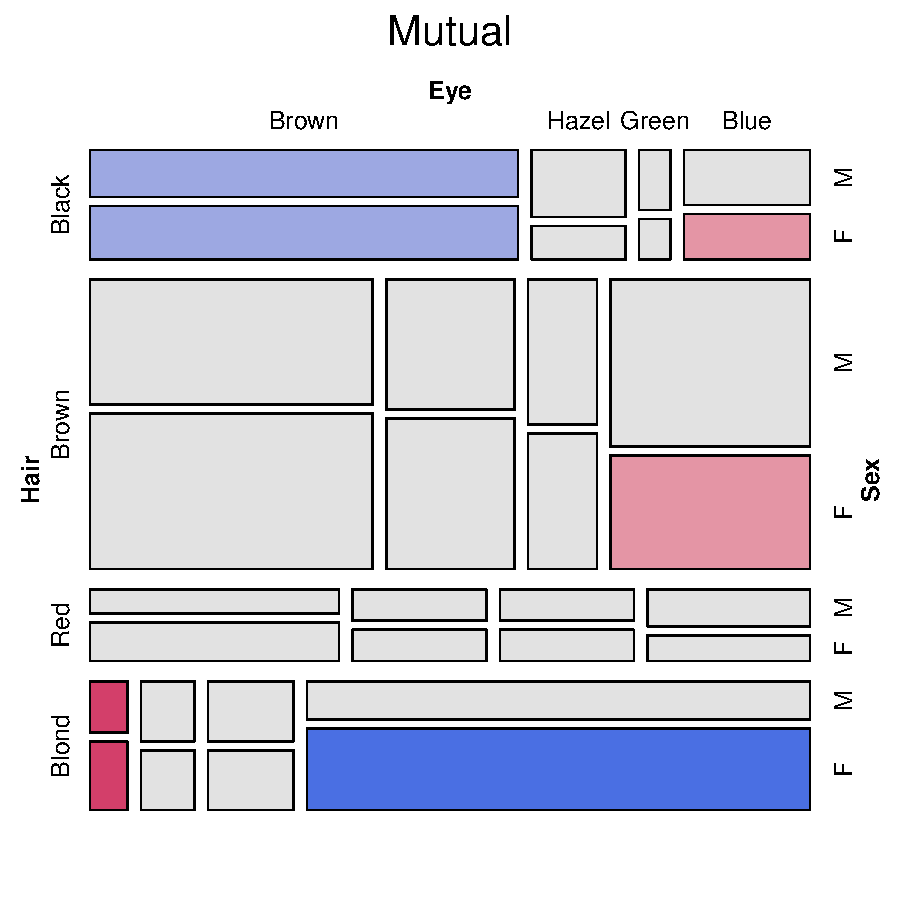
\includegraphics[width=1\linewidth,clip]{ch05/fig/HEC-seq1}
  \\ \centering [Hair] [Eye] [Sex]
  \\ \centering $G^2_{(24)} = 166.30$
 \end{minipage}%
 \hfill {\Huge =} \hfill
 \begin{minipage}[c]{.3\textwidth}
%  \centering Marginal
  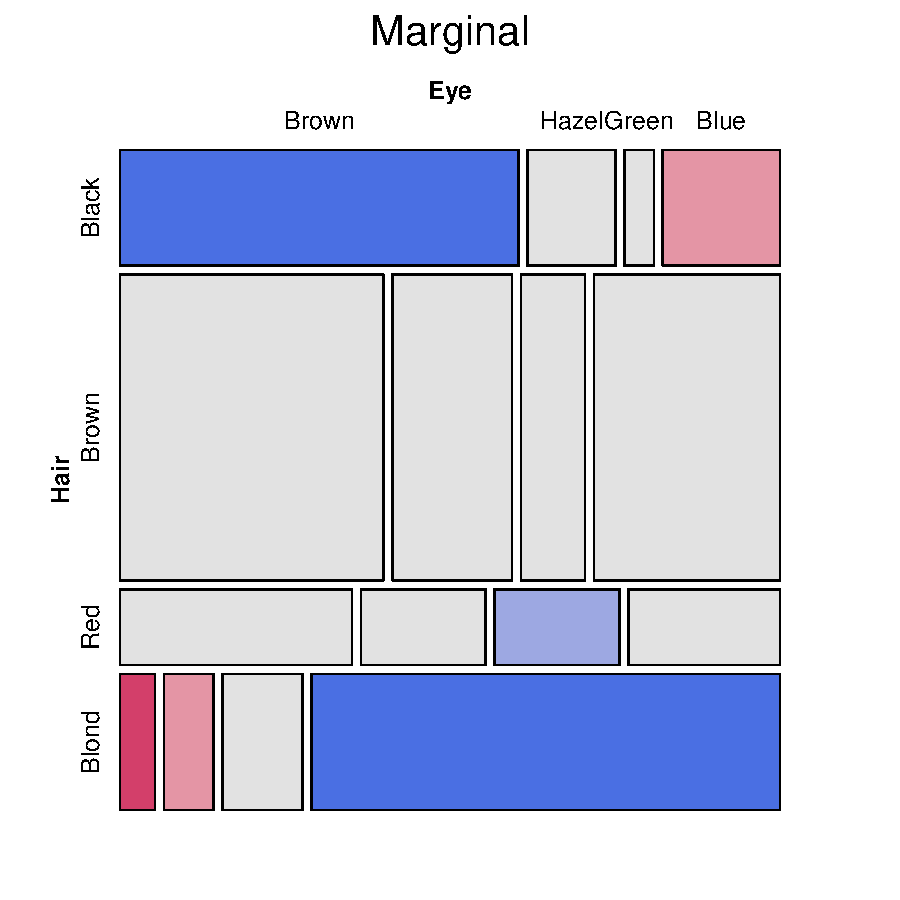
\includegraphics[width=1\linewidth,clip]{ch05/fig/HEC-seq2}
  \\ \centering [Hair] [Eye]
  \\ \centering $G^2_{(9)} = 146.44$
 \end{minipage}
 \hfill {\Huge +} \hfill
 \begin{minipage}[c]{.3\textwidth}
%  \centering Joint
  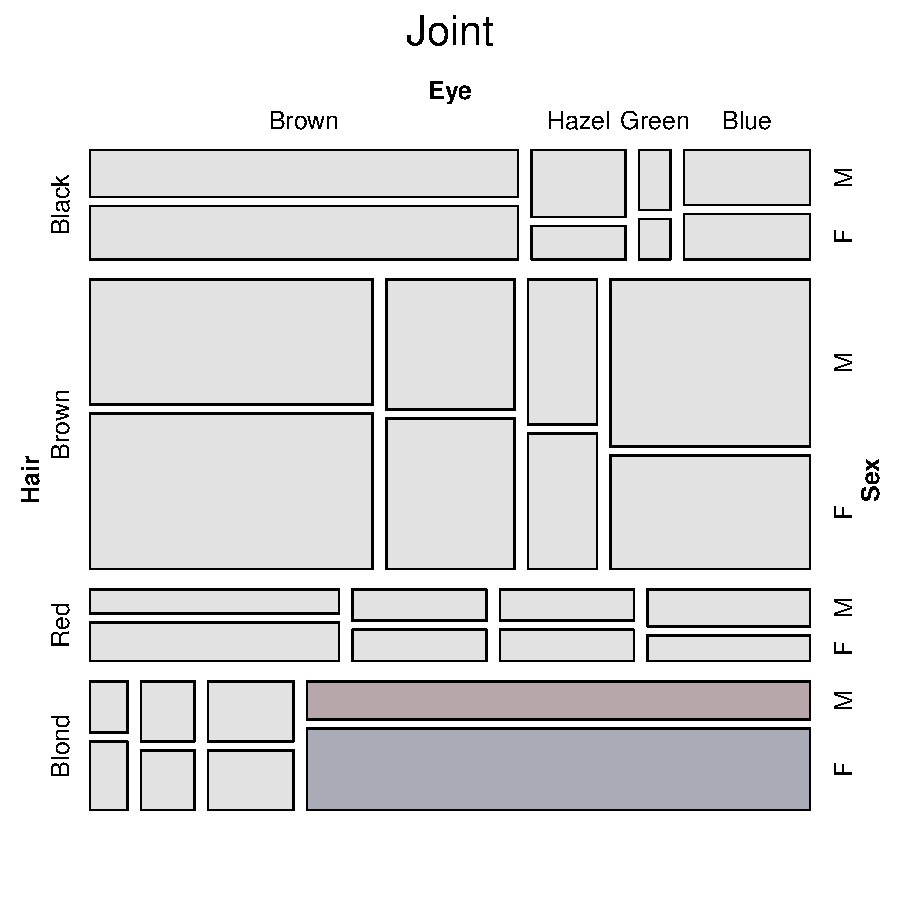
\includegraphics[width=1\linewidth,clip]{ch05/fig/HEC-seq3}
  \\ \centering [Hair Eye] [Sex]
  \\ \centering $G^2_{(15)} = 19.86$
 \end{minipage}
 \caption{Visual representation of the decomposition of the $\GSQ$ for mutual independence (total)
 as the sum of marginal and joint independence.}
 \label{fig:HEC-seq}
\end{figure}

Although sequential models of joint independence have the nice additive property illustrated
above, other classes of sequential models are possible, and sometimes of substantive interest.
The main types of these models are illustrated in \tabref{tab:seqmodels} for 3-, 4-, and 5-
way tables, with variables A, B, ... E.  In all cases, the natural model for the one-way
margin is the equiprobability model, and that for the two-way margin is \LLM{A,B}.

\begin{table}[htb]
\caption[Sequential models]{Classes of sequential models for \nway tables}\label{tab:seqmodels}
\begin{center}
\begin{tabular}{llll} 
\hline
\tableheader
\textbf{\code{function}} & \textbf{3-way} & \textbf{4-way} & \textbf{5-way} \\ 
\hline
\code{mutual} &  [A]  [B]  [C]  &
             [A]  [B]  [C]  [D]  &
             [A]  [B]  [C]  [D]  [E] \\ 
\code{joint}  &  [AB]  [C]  &
             [ABC]  [D]  &
             [ABCE]  [E]  \\ 
\code{joint (with=1)} & 
             [A]  [BC]  &
             [A]  [BCD]  &
             [A]  [BCDE]  \\ 
\code{conditional}  & 
             [AC]  [BC]  & 
             [AD]  [BD]  [CD]  &
             [AE]  [BE]  [CE]  [DE] \\ 
\code{conditional (with=1)}  & 
             [AB]  [AC]  & 
             [AB]  [AC]  [AD]  &
             [AB]  [AC]  [AD]  [AE] \\ 
\code{markov (order=1)}  &  
             [AB]  [BC]  &
             [AB]  [BC]  [CD]  &
             [AB]  [BC]  [CD]  [DE] \\ 
\code{markov (order=2)}  & 
             [A]  [B]  [C]  &
             [ABC]  [BCD]  &
             [ABC]  [BCD]  [CDE]  \\
\code{saturated}  &
             [ABC] & [ABCD] & [ABCDE] \\
\hline
\end{tabular}
\end{center}
\end{table}

The \Rpackage{vcdExtra} provides a collection of convenience functions that generate
the \loglin model formulae symbolically, as indicated in the \textbf{function} column.
The functions \func{mutual}, \func{joint}, \func{conditional}, \func{markov}
and so forth simply
generate a list of terms suitable for a model formula for \func{loglin}.
See \help{loglin-utilities} for further details.

Wrapper functions \func{loglin2string} and \func{loglin2formula}
convert these to character strings or model formulae respectively,
for use with \func{loglm} and \func{mosaic}-related functions in
\pkg{vcdExtra}.  Some examples are shown below.

\begin{knitrout}
\definecolor{shadecolor}{rgb}{1, 0.961, 0.933}\color{fgcolor}\begin{kframe}
\begin{alltt}
\hlstd{> }\hlkwa{for}\hlstd{(nf} \hlkwa{in} \hlnum{2} \hlopt{:} \hlnum{5}\hlstd{) \{}
\hlstd{+ }  \hlkwd{print}\hlstd{(}\hlkwd{loglin2string}\hlstd{(}\hlkwd{joint}\hlstd{(nf,} \hlkwc{factors} \hlstd{= LETTERS[}\hlnum{1}\hlopt{:}\hlnum{5}\hlstd{])))}
\hlstd{+ }\hlstd{\}}
\end{alltt}
\begin{verbatim}
[1] "[A] [B]"
[1] "[A,B] [C]"
[1] "[A,B,C] [D]"
[1] "[A,B,C,D] [E]"
\end{verbatim}
\begin{alltt}
\hlstd{> }\hlkwa{for}\hlstd{(nf} \hlkwa{in} \hlnum{2} \hlopt{:} \hlnum{5}\hlstd{) \{}
\hlstd{+ }  \hlkwd{print}\hlstd{(}\hlkwd{loglin2string}\hlstd{(}\hlkwd{conditional}\hlstd{(nf,} \hlkwc{factors} \hlstd{= LETTERS[}\hlnum{1}\hlopt{:}\hlnum{5}\hlstd{]),} \hlkwc{sep} \hlstd{=} \hlstr{""}\hlstd{))}
\hlstd{+ }\hlstd{\}}
\end{alltt}
\begin{verbatim}
[1] "[A] [B]"
[1] "[AC] [BC]"
[1] "[AD] [BD] [CD]"
[1] "[AE] [BE] [CE] [DE]"
\end{verbatim}
\begin{alltt}
\hlstd{> }\hlkwa{for}\hlstd{(nf} \hlkwa{in} \hlnum{2} \hlopt{:} \hlnum{5}\hlstd{) \{}
\hlstd{+ }  \hlkwd{print}\hlstd{(}\hlkwd{loglin2formula}\hlstd{(}\hlkwd{conditional}\hlstd{(nf,} \hlkwc{factors} \hlstd{= LETTERS[}\hlnum{1}\hlopt{:}\hlnum{5}\hlstd{])))}
\hlstd{+ }\hlstd{\}}
\end{alltt}
\begin{verbatim}
~A + B
~A:C + B:C
~A:D + B:D + C:D
~A:E + B:E + C:E + D:E
\end{verbatim}
\end{kframe}
\end{knitrout}
Applied to data, these functions take a \argument{table}, and deliver
the string or formula representation of a type of model for that table:
\begin{knitrout}
\definecolor{shadecolor}{rgb}{1, 0.961, 0.933}\color{fgcolor}\begin{kframe}
\begin{alltt}
\hlstd{> }\hlkwd{loglin2formula}\hlstd{(}\hlkwd{joint}\hlstd{(}\hlnum{3}\hlstd{,} \hlkwc{table} \hlstd{= HEC))}
\end{alltt}
\begin{verbatim}
~Hair:Eye + Sex
\end{verbatim}
\begin{alltt}
\hlstd{> }\hlkwd{loglin2string}\hlstd{(}\hlkwd{joint}\hlstd{(}\hlnum{3}\hlstd{,} \hlkwc{table} \hlstd{= HEC))}
\end{alltt}
\begin{verbatim}
[1] "[Hair,Eye] [Sex]"
\end{verbatim}
\end{kframe}
\end{knitrout}
Their main use, however, is within higher-level functions,
such as \func{seq\_loglm}, which fit the collection of sequential models
of a given type.
\begin{knitrout}
\definecolor{shadecolor}{rgb}{1, 0.961, 0.933}\color{fgcolor}\begin{kframe}
\begin{alltt}
\hlstd{> }\hlstd{HEC.mods} \hlkwb{<-} \hlkwd{seq_loglm}\hlstd{(HEC,} \hlkwc{type} \hlstd{=} \hlstr{"joint"}\hlstd{)}
\hlstd{> }\hlkwd{LRstats}\hlstd{(HEC.mods)}
\end{alltt}
\begin{verbatim}
Likelihood summary table:
        AIC BIC LR Chisq Df Pr(>Chisq)    
model.1 194 194    165.6  3     <2e-16 ***
model.2 241 246    146.4  9     <2e-16 ***
model.3 193 218     19.9 15       0.18    
---
Signif. codes:  0 '***' 0.001 '**' 0.01 '*' 0.05 '.' 0.1 ' ' 1
\end{verbatim}
\end{kframe}
\end{knitrout}

In this section we have described a variety of models which can be fit
to higher-way tables, some relations among those models, and the aspects
of lack-of-fit which are revealed in the mosaic displays.
The following examples illustrate the process of model fitting,
using the mosaic as an interpretive guide to the nature of associations
among the variables.
In general, we start with a minimal baseline model.%
%
\footnote{When one variable, $R$
is a response, this normally is the model of joint independence,
\([E_1 E_2 \dots] \, [R]\), where \(E_1, E_2, \dots\) are the explanatory
variables.  Better-fitting models will often include associations
of the form \([E_i \, R]\), \([E_i \, E_j \, R] \dots \).
}
The pattern of residuals in the mosaic will suggest associations to be added
to an adequate explanatory model.
As the model achieves better fit to the data, the degree of shading
decreases, so we may think of the process of model fitting as
``cleaning the mosaic.''

\subsection{Causal models}\label{sec:causal}

The sequence of models of joint independence has another
interpretation when the ordering of the variables is based on a set
of ordered hypotheses involving causal relationships among
variables
(\citet{Goodman:73}, \citet[\S 7.2]{Fienberg:80}).  Suppose, for example,
that the causal ordering of four variables is \(A \rightarrow B
\rightarrow C \rightarrow D\), where the arrow means ``is antecedent
to.''  Goodman suggests that the conditional joint probabilities of
$B$, $C$, and $D$ given $A$ can be characterized by a set of
recursive logit models which treat
\begin{seriate}
\item $B$ as a response to $A$,
\item $C$
as a response to $A$ and $B$ jointly,
\item and $D$ as a response to $A$,
$B$ and $C$.
\end{seriate}
These are equivalent to the \loglin models which
we fit as the sequential baseline models of joint independence,
namely \LLM{A,B}, \LLM{AB,C}, and \LLM{ABC,D}.  The combination of these
models with the marginal probabilities of A gives a characterization
of the joint probabilities of all four variables, as in \eqref{eq:seqprod}.
In application, residuals from each submodel show the associations that
remain unexplained.

\begin{Example}[marital1]{Marital status and pre- and extramarital sex}

A study of divorce patterns in relation to premarital and extramarital sex
by \citet{ThornesCollard:79} reported
the \(2^4\) table shown below, and included in \pkg{vcd} as
\data{PreSex}.
%in  \tabref{tab:maridat}.

\begin{knitrout}
\definecolor{shadecolor}{rgb}{1, 0.961, 0.933}\color{fgcolor}\begin{kframe}
\begin{alltt}
\hlstd{> }\hlkwd{data}\hlstd{(}\hlstr{"PreSex"}\hlstd{,} \hlkwc{package} \hlstd{=} \hlstr{"vcd"}\hlstd{)}
\hlstd{> }\hlkwd{structable}\hlstd{(Gender} \hlopt{+} \hlstd{PremaritalSex} \hlopt{+} \hlstd{ExtramaritalSex} \hlopt{~} \hlstd{MaritalStatus, PreSex)}
\end{alltt}
\begin{verbatim}
              Gender          Women             Men            
              PremaritalSex     Yes      No     Yes      No    
              ExtramaritalSex   Yes  No Yes  No Yes  No Yes  No
MaritalStatus                                                  
Divorced                         17  54  36 214  28  60  17  68
Married                           4  25   4 322  11  42   4 130
\end{verbatim}
\end{kframe}
\end{knitrout}

These data were analysed by \citet[\S 6.1.7]{Agresti:2013}
and by \citet{Friendly:94a,Friendly:00:VCD}, from which this account draws.
A sample of
about 500 people who had petitioned for divorce, and a similar number
of married people were asked two questions regarding their pre- and
extramarital sexual experience:  (1) ``Before you married your
(former) husband/wife, had you ever made love with anyone else?,''
(2) ``During your (former) marriage (did you) have you had any
affairs or brief sexual encounters with another man/woman?''
The
table variables are thus gender ($G$), reported premarital ($P$)
and extramarital ($E$) sex, and current marital status ($M$).

In this analysis we consider the variables in the order $G$, $P$,
$E$, and $M$, and first reorder the table variables for
convenience.
\begin{knitrout}
\definecolor{shadecolor}{rgb}{1, 0.961, 0.933}\color{fgcolor}\begin{kframe}
\begin{alltt}
\hlstd{> }\hlstd{PreSex} \hlkwb{<-} \hlkwd{aperm}\hlstd{(PreSex,} \hlnum{4} \hlopt{:} \hlnum{1}\hlstd{)}   \hlcom{# order variables G, P, E, M}
\end{alltt}
\end{kframe}
\end{knitrout}


That is, the first stage  treats $P$ as a
response to $G$ and examines the [Gender][Pre] mosaic to assess
whether gender has an effect on premarital sex.  The second stage
treats $E$ as a response to $G$ and $P$ jointly;  the
mosaic for [Gender, Pre] [Extra] shows whether extramarital sex
is related to either gender or premarital sex.  These are shown
in \figref{fig:presex2}.

\begin{knitrout}
\definecolor{shadecolor}{rgb}{1, 0.961, 0.933}\color{fgcolor}\begin{kframe}
\begin{alltt}
\hlstd{> }\hlcom{# (Gender Pre)}
\hlstd{> }\hlkwd{mosaic}\hlstd{(}\hlkwd{margin.table}\hlstd{(PreSex,} \hlnum{1} \hlopt{:} \hlnum{2}\hlstd{),} \hlkwc{shade} \hlstd{=} \hlnum{TRUE}\hlstd{,}
\hlstd{+ }                \hlkwc{main} \hlstd{=} \hlstr{"Gender and Premarital Sex"}\hlstd{)}
\hlstd{> }
\hlstd{> }\hlcom{## (Gender Pre)(Extra)}
\hlstd{> }\hlkwd{mosaic}\hlstd{(}\hlkwd{margin.table}\hlstd{(PreSex,} \hlnum{1} \hlopt{:} \hlnum{3}\hlstd{),}
\hlstd{+ }       \hlkwc{expected} \hlstd{=} \hlopt{~} \hlstd{Gender} \hlopt{*} \hlstd{PremaritalSex} \hlopt{+} \hlstd{ExtramaritalSex ,}
\hlstd{+ }       \hlkwc{main} \hlstd{=} \hlstr{"Gender*Pre + ExtramaritalSex"}\hlstd{)}
\end{alltt}
\end{kframe}\begin{figure}[!htbp]

\centerline{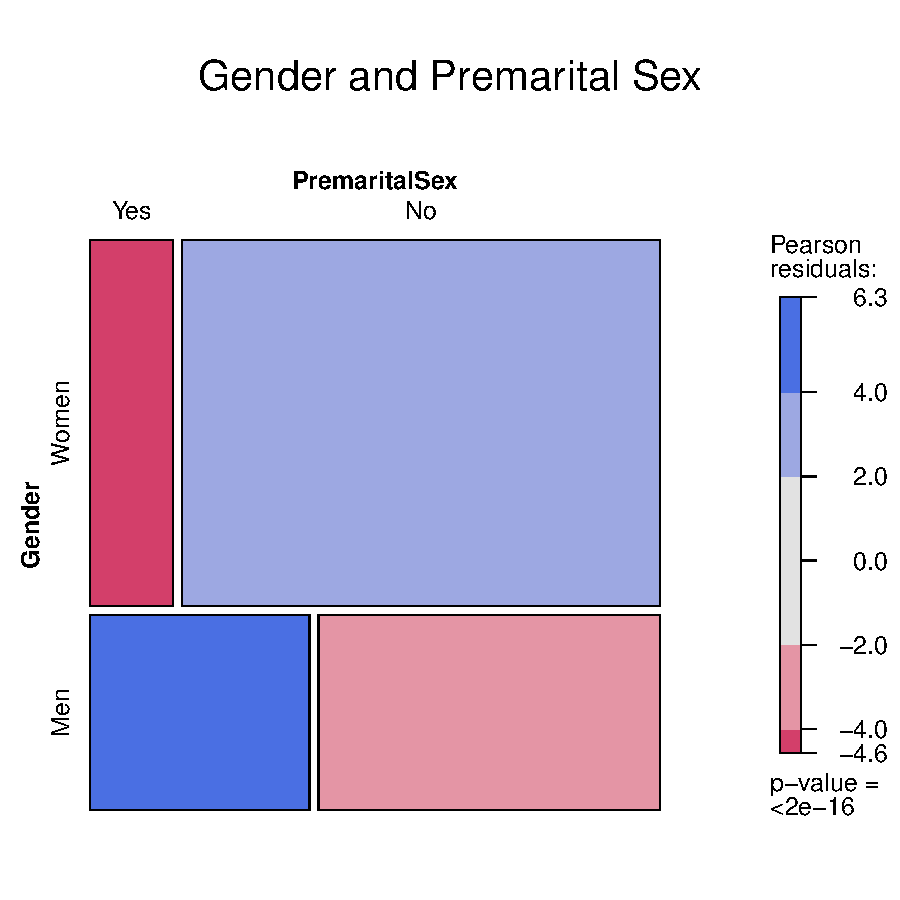
\includegraphics[width=.49\textwidth]{ch05/fig/presex2-1} 
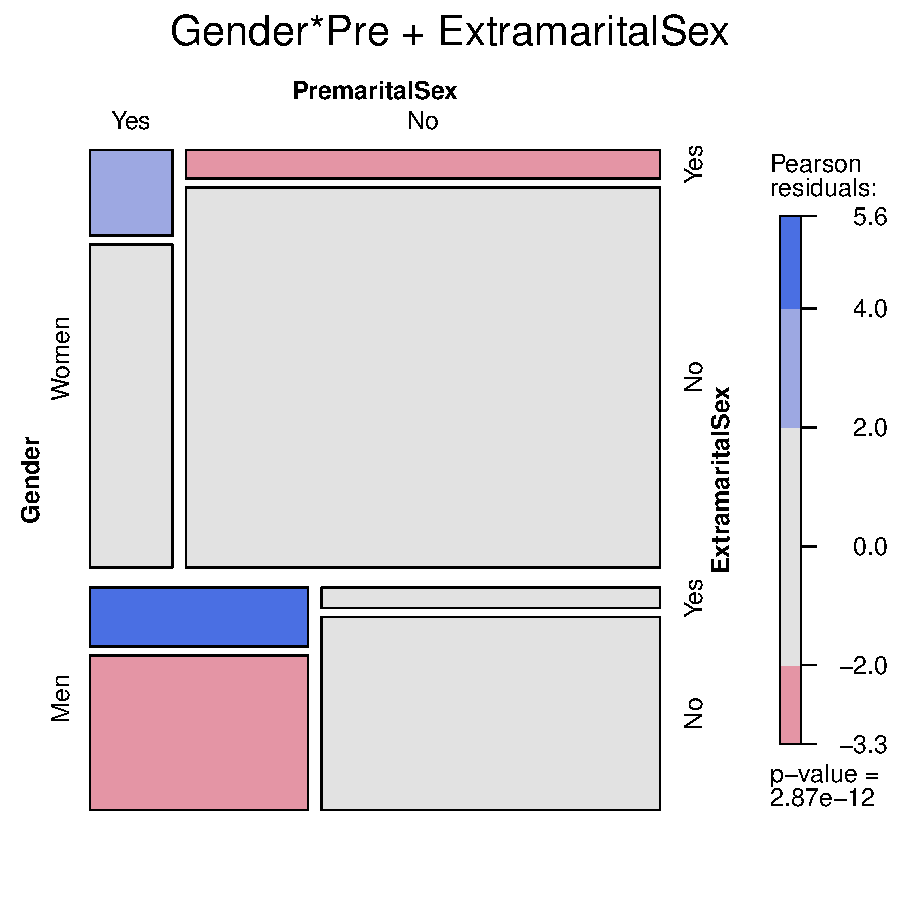
\includegraphics[width=.49\textwidth]{ch05/fig/presex2-2} }

\caption[Mosaic displays for the first two marginal tables in the PreSex data]{Mosaic displays for the first two marginal tables in the PreSex data. Left: Gender and premarital sex; right: fitting the model of joint independence with extramarital sex, [GP][E]\label{fig:presex2}}
\end{figure}


\end{knitrout}

Finally, the mosaic
for [Gender, Pre, Extra] [Marital] is examined for evidence of the
dependence of marital status on the three previous variables jointly.
As noted above, these models are equivalent to the
recursive logit models whose path diagram is \(G \rightarrow P
\rightarrow E \rightarrow M\).%
\footnote{ \citet[Figure 6.1]{Agresti:2013} considers a slightly more complex,
but more realistic model in which premarital sex affects both the propensity
to have extramarital sex and subsequent marital status.}
The \(G^2\) values for these models
shown below provide a decomposition of the
\(G^2\) for the model of complete independence fit to the full table.

\begin{center}
 \begin{tabular}{rrr}
 \hline
  Model        & df & \(G^2\) \\
 \hline
  \llmtwo{G}{P}    & 1  & 75.259 \\
  \llmtwo{GP}{E}   & 3  & 48.929 \\
  \llmtwo{GPE}{M}  & 7  & 107.956 \\
 \hline
  \llmfour{G}{P}{E}{M} & 11 & 232.142 \\
 \hline
 \end{tabular}
\end{center}

The [Gender] [Pre] mosaic in the left panel of \figref{fig:presex2}
shows that men are much more likely to report
premarital sex than are women; the sample odds ratio is 3.7.  We
also see that women are about twice as prevalent as men in this
sample.  The mosaic for the model of joint independence,
[Gender Pre] [Extra] in the right panel of \figref{fig:presex2}
shows that extramarital sex
depends on gender and premarital sex jointly.
From the pattern
of residuals in \figref{fig:presex2} we see that men and
women who have reported premarital sex are far more likely to report
extramarital sex than those who have not.
In this three-way marginal table,
the conditional odds ratio of extramarital
sex given premarital sex is nearly the same for both genders
(3.61 for men and 3.56 for women).  Thus, extramarital sex
depends on premarital sex, but not on gender.

\begin{knitrout}
\definecolor{shadecolor}{rgb}{1, 0.961, 0.933}\color{fgcolor}\begin{kframe}
\begin{alltt}
\hlstd{> }\hlkwd{oddsratio}\hlstd{(}\hlkwd{margin.table}\hlstd{(PreSex,} \hlnum{1} \hlopt{:} \hlnum{3}\hlstd{),} \hlkwc{stratum} \hlstd{=} \hlnum{1}\hlstd{,} \hlkwc{log} \hlstd{=} \hlnum{FALSE}\hlstd{)}
\end{alltt}
\begin{verbatim}
Women   Men 
3.562 3.605 
\end{verbatim}
\end{kframe}
\end{knitrout}



\begin{knitrout}
\definecolor{shadecolor}{rgb}{1, 0.961, 0.933}\color{fgcolor}\begin{kframe}
\begin{alltt}
\hlstd{> }\hlcom{## (Gender Pre Extra)(Marital)}
\hlstd{> }\hlkwd{mosaic}\hlstd{(PreSex,}
\hlstd{+ }       \hlkwc{expected} \hlstd{=} \hlopt{~} \hlstd{Gender} \hlopt{*} \hlstd{PremaritalSex} \hlopt{*} \hlstd{ExtramaritalSex}
\hlstd{+ }                  \hlopt{+} \hlstd{MaritalStatus,}
\hlstd{+ }       \hlkwc{main} \hlstd{=} \hlstr{"Gender*Pre*Extra + MaritalStatus"}\hlstd{)}
\hlstd{> }\hlcom{## (GPE)(PEM)}
\hlstd{> }\hlkwd{mosaic}\hlstd{(PreSex,}
\hlstd{+ }       \hlkwc{expected} \hlstd{=} \hlopt{~} \hlstd{Gender} \hlopt{*} \hlstd{PremaritalSex} \hlopt{*} \hlstd{ExtramaritalSex}
\hlstd{+ }                  \hlopt{+} \hlstd{MaritalStatus} \hlopt{*} \hlstd{PremaritalSex} \hlopt{*} \hlstd{ExtramaritalSex,}
\hlstd{+ }       \hlkwc{main} \hlstd{=} \hlstr{"G*P*E + P*E*M"}\hlstd{)}
\end{alltt}
\end{kframe}\begin{figure}[!htbp]

\centerline{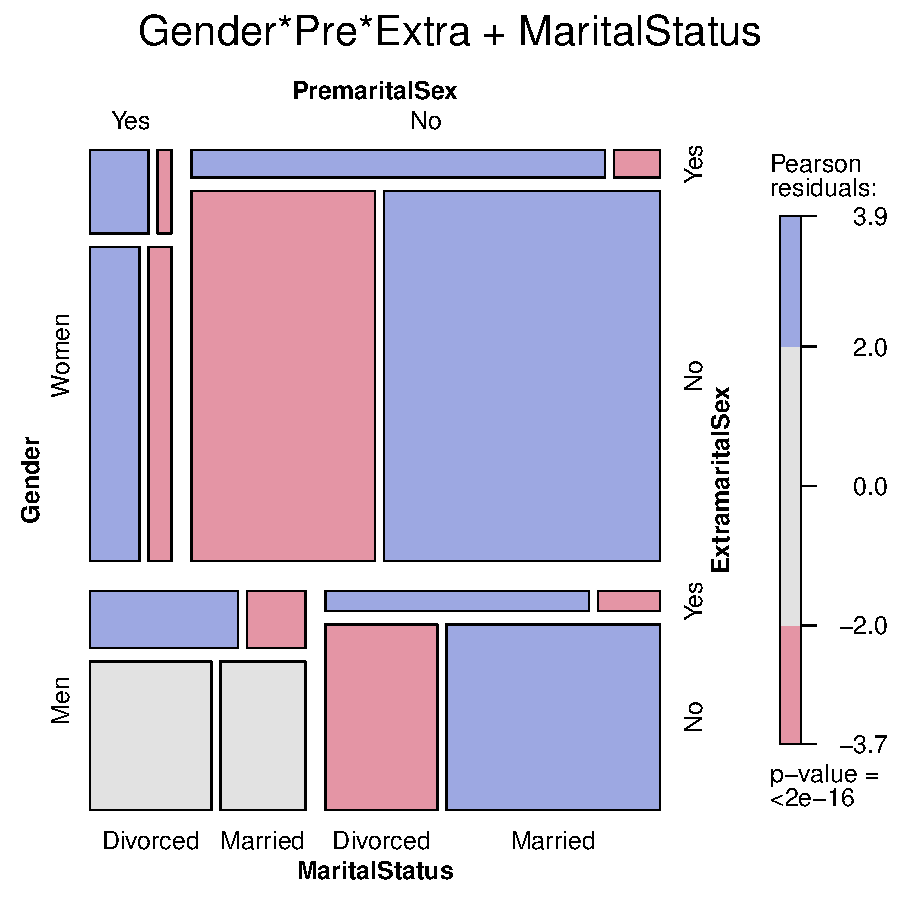
\includegraphics[width=.49\textwidth]{ch05/fig/presex3-1} 
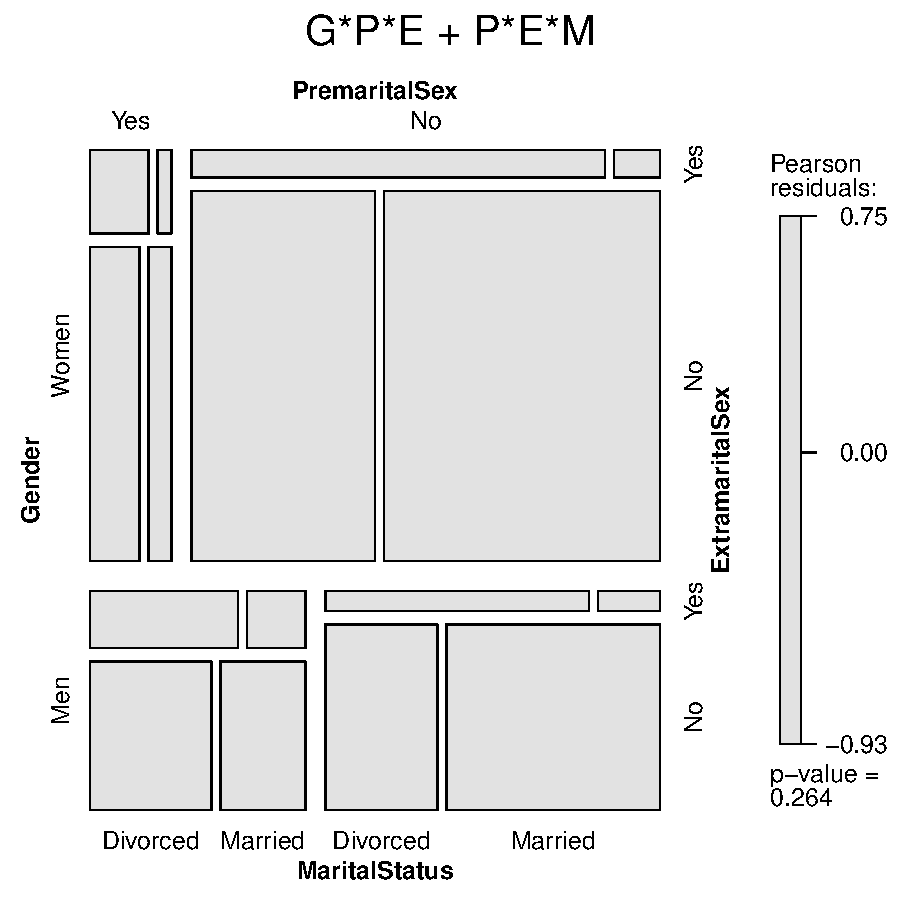
\includegraphics[width=.49\textwidth]{ch05/fig/presex3-2} }

\caption[Four-way mosaics for the PreSex data]{Four-way mosaics for the PreSex data. The left panel fits the model [GPE][M]. The pattern of residuals suggests other associations with marital status. The right panel fits the model [GPE][PEM]\label{fig:presex3}}
\end{figure}


\end{knitrout}

\end{Example}

\TODO{Complete this section with other examples: Titanic }

\subsection{Partial association}\label{sec:mospart}

In a three-way (or larger) table it may be that two variables, say $A$ and $B$, are
associated at some levels of the third variable, $C$, but not at other
levels of $C$. More generally, we may wish to explore whether and how the
association among two (or more) variables in a contingency table varies over
the levels of the remaining variables. The term \term{partial association} refers
to the association among some variables within the levels of the other
variables.

Partial association represents a useful ``divide and conquer'' statistical strategy:
it allows you to refine the question you want to answer for complex relations
by breaking it down to smaller, easier questions.%
\footnote{
This is an analog, for categorical data, of the ANOVA strategy for ``probing interactions''
by testing \term{simple effects} at the levels of one or more of the
factors involved in a two- or higher-way interaction.
}
It is a statistically
happy fact that an answer to the larger, more complex question
can be expressed as an algebraic sum of the answers to the smaller questions,
just as was the case with sequential models of joint independence.

For concreteness, consider the case where you want to understand the
relationship between \emph{attitude} toward corporal punishment of children
by parents or teachers (Never, Moderate use OK) and \emph{memory}
that the respondent had experiences corporal punishment as a child (Yes, No).
But you also have measured other variables on the respondents, including their
level of \emph{education} and \emph{age} category.  In this case, the
question of association among all the table variables may be complex,
but we can answer a highly relevant, specialized question
precisely,
``is there an association between attitude and memory,
\emph{controlling for education and age}?''
The answer to this question can be thought of as the sum of the
answers to the simpler question of association between attitude and memory
across the education, age categories.

A simpler version of this idea is considered first below (\exref{ex:employ}):
among workers who were laid off
due to either the closure of a plant or business vs.
replacement by another worker,
the (conditional)
relationship of employment status (new job vs. still unemployed)
and duration of unemployment can be studied as a sum of the
associations between these focal variables over the separate tables
for cause of layoff.

To make this idea precise, consider for example the model of conditional independence, $A\perp B\given C$
for a three-way table. This model asserts that $A$ and $B$ are independent
within \textit{each} level of $C$. Denote the hypothesis that $A$ and $B$
are independent at level $C(k)$ by $A\perp B\given C(k), k=1, \dots K$. Then one can show
\citep{Andersen:91} that

\begin{equation}\label{eq:partial1}
G_{A\perp B\given C}^2=\sum_k^K G_{A\perp B\given C(k)}^2
\end{equation}
That is, the overall likelihood ratio \GSQ for the conditional independence model
with $(I-1)(J-1)K$ \df{} is the
sum of the values for the ordinary association between $A$ and $B$ over the levels of
$C$ (each with $(I-1)(J-1)$ \df{}). The same additive relationship holds for the
Pearson $\chi^2$ statistics: $\chi^2_{A\perp B\given C}=\sum_k^K \chi^2_{A\perp B\given C(k)}$.

Thus,
\begin{seriate}
\item the overall \GSQ (\chisq) may be decomposed into portions attributable
to the $AB$ association in the layers of $C$, and
\item the collection of mosaic displays for the dependence of $A$ and $B$
for each of the levels of $C$ provides a natural visualization of this
decomposition.  These provide an analog, for categorical data, of the conditioning plot, or
\term{coplot}, that
\citet{Cleveland:VisData} has shown to be an effective display for
quantitative data.
\end{seriate}
See \citet{Friendly:99b} for further details.

Mosaic and other displays in the strucplot framework
for partial association can be produced in several different ways.
One way is to use a model formula in the call to \func{mosaic}
which lists the conditioning variables after the \code{"|"}
(given) symbol,
as in
\linebreak \url{~ Memory + Attitude | Age + Education}.
Another way is to use \func{cotabplot}. This takes the same
kind of conditioning model formula, but presents each panel for
the conditioning variables in a separate frame within a
 trellis-like grid.%
 \footnote{
 Depending on your perspective, this has the advantage of adjusting
 for the total frequency in each conditional panel, or
 the disadvantage of ignoring these differences.
 }

\begin{Example}[employ]{Employment status data}
Data from a 1974 Danish study of 1314 employees who had been laid off
are given in the data table \data{Employment} in \pkg{vcd}
(from \citet[Table 5.12]{Andersen:91}).
The workers are classified by:
\begin{seriate}
\item their employment status, on January 1, 1975 (\code{"NewJob"} or still \code{"Unemployed}),
\item the length of their employment at the time of layoff,
\item the cause of their layoff (\code{"Closure"}, etc. or \code{"Replaced"}).
\end{seriate}

\begin{knitrout}\footnotesize
\definecolor{shadecolor}{rgb}{1, 0.961, 0.933}\color{fgcolor}\begin{kframe}
\begin{alltt}
\hlstd{> }\hlkwd{data}\hlstd{(}\hlstr{"Employment"}\hlstd{,} \hlkwc{package} \hlstd{=} \hlstr{"vcd"}\hlstd{)}
\hlstd{> }\hlkwd{structable}\hlstd{(Employment)}
\end{alltt}
\begin{verbatim}
                             EmploymentLength <1Mo 1-3Mo 3-12Mo 1-2Yr 2-5Yr >5Yr
EmploymentStatus LayoffCause                                                    
NewJob           Closure                         8    35     70    62    56   38
                 Replaced                       40    85    181    85   118   56
Unemployed       Closure                        10    42     86    80    67   35
                 Replaced                       24    42     41    16    27   10
\end{verbatim}
\end{kframe}
\end{knitrout}

In this example, it is natural to regard \code{EmploymentStatus} (variable $A$)
as the response variable,
and \code{EmploymentLength} ($B$) and \code{LayoffCause} ($C$) as predictors.
In this case, the minimal baseline model is the joint independence model,
\([A] \,  [BC] \), which asserts that  employment status is independent of both
length and cause.
This model fits quite poorly, as shown in the output from \func{loglm} below.
\begin{knitrout}
\definecolor{shadecolor}{rgb}{1, 0.961, 0.933}\color{fgcolor}\begin{kframe}
\begin{alltt}
\hlstd{> }\hlkwd{loglm}\hlstd{(}\hlopt{~} \hlstd{EmploymentStatus} \hlopt{+} \hlstd{EmploymentLength} \hlopt{*} \hlstd{LayoffCause,} \hlkwc{data} \hlstd{= Employment)}
\end{alltt}
\begin{verbatim}
Call:
loglm(formula = ~EmploymentStatus + EmploymentLength * LayoffCause, 
    data = Employment)

Statistics:
                    X^2 df P(> X^2)
Likelihood Ratio 172.28 11        0
Pearson          165.70 11        0
\end{verbatim}
\end{kframe}
\end{knitrout}

The residuals, shown in \figref{fig:employ-mos1},
indicate an opposite pattern for the two categories of \code{LayoffCause}:
those who were laid off as a result of a closure
are more likely to be unemployed, regardless of length of time
they were employed.
Workers who were replaced, however, apparently are more likely
to be employed, particularly if they were employed for 3 months or more.

\begin{knitrout}
\definecolor{shadecolor}{rgb}{1, 0.961, 0.933}\color{fgcolor}\begin{kframe}
\begin{alltt}
\hlstd{> }\hlcom{# baseline model [A][BC]}
\hlstd{> }\hlkwd{mosaic}\hlstd{(Employment,} \hlkwc{shade} \hlstd{=} \hlnum{TRUE}\hlstd{,}
\hlstd{+ }       \hlkwc{expected} \hlstd{=} \hlopt{~} \hlstd{EmploymentStatus} \hlopt{+} \hlstd{EmploymentLength} \hlopt{*} \hlstd{LayoffCause,}
\hlstd{+ }       \hlkwc{main} \hlstd{=} \hlstr{"EmploymentStatus + Length * Cause"}\hlstd{)}
\end{alltt}
\end{kframe}\begin{figure}[!htbp]

\centerline{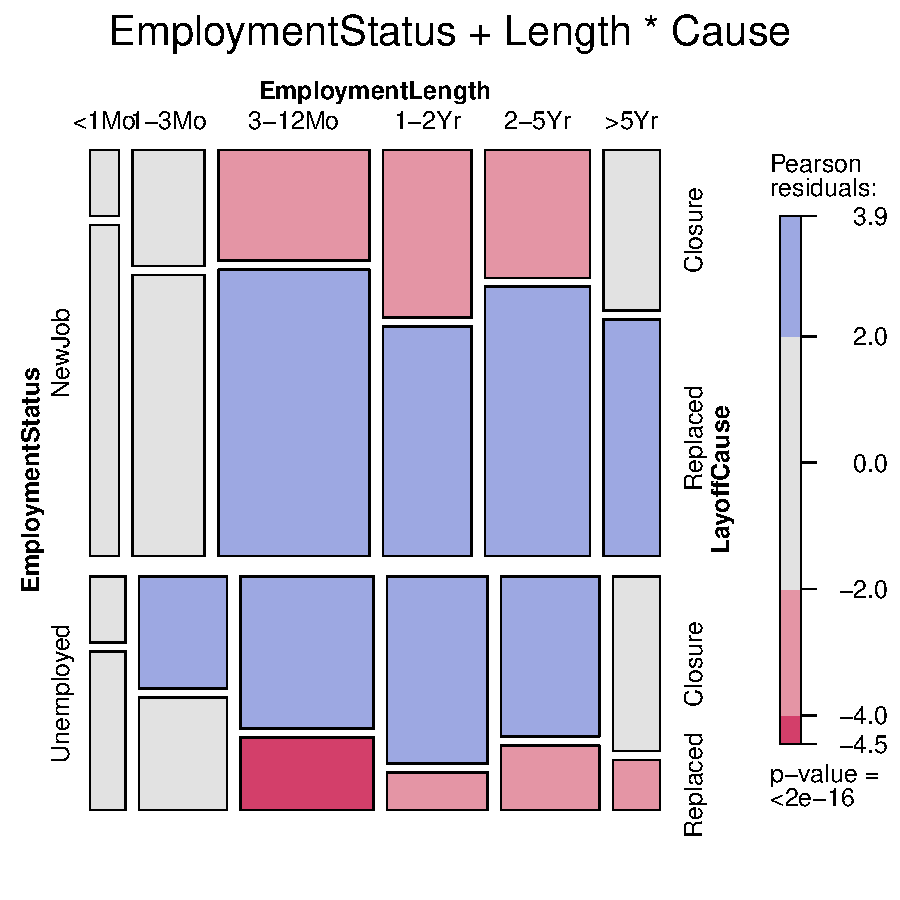
\includegraphics[width=.6\textwidth]{ch05/fig/employ-mos1-1} }

\caption[Mosaic display for the employment status data, fitting the baseline model of joint independence]{Mosaic display for the employment status data, fitting the baseline model of joint independence.\label{fig:employ-mos1}}
\end{figure}


\end{knitrout}

Beyond this baseline model, it is substantively more meaningful to consider the
conditional independence model, \(A \perp B \given C\),
(or \LLM{AC,BC} in shorthand notation), which asserts that
employment status is independent of length of employment, given the cause of layoff.
We fit this model as shown below:
\begin{knitrout}
\definecolor{shadecolor}{rgb}{1, 0.961, 0.933}\color{fgcolor}\begin{kframe}
\begin{alltt}
\hlstd{> }\hlkwd{loglm}\hlstd{(}\hlopt{~} \hlstd{EmploymentStatus} \hlopt{*} \hlstd{LayoffCause} \hlopt{+} \hlstd{EmploymentLength} \hlopt{*} \hlstd{LayoffCause,}
\hlstd{+ }      \hlkwc{data} \hlstd{= Employment)}
\end{alltt}
\begin{verbatim}
Call:
loglm(formula = ~EmploymentStatus * LayoffCause + EmploymentLength * 
    LayoffCause, data = Employment)

Statistics:
                    X^2 df  P(> X^2)
Likelihood Ratio 24.630 10 0.0060927
Pearson          26.072 10 0.0036445
\end{verbatim}
\end{kframe}
\end{knitrout}
This model fits far better (\(G^2 (10) = 24.63\)),
but the lack of fit is still significant.
The residuals, shown in \figref{fig:employ-mos2}, still
suggest that the pattern of association between employment and length
is different for replaced workers and those laid off due to closure of their workplace.

\begin{knitrout}
\definecolor{shadecolor}{rgb}{1, 0.961, 0.933}\color{fgcolor}\begin{kframe}
\begin{alltt}
\hlstd{> }\hlkwd{mosaic}\hlstd{(Employment,} \hlkwc{shade} \hlstd{=} \hlnum{TRUE}\hlstd{,} \hlkwc{gp_args} \hlstd{=} \hlkwd{list}\hlstd{(}\hlkwc{interpolate} \hlstd{=} \hlnum{1} \hlopt{:} \hlnum{4}\hlstd{),}
\hlstd{+ }       \hlkwc{expected} \hlstd{=} \hlopt{~} \hlstd{EmploymentStatus} \hlopt{*} \hlstd{LayoffCause} \hlopt{+} \hlstd{EmploymentLength} \hlopt{*} \hlstd{LayoffCause,}
\hlstd{+ }       \hlkwc{main} \hlstd{=} \hlstr{"EmploymentStatus * Cause + Length * Cause"}\hlstd{)}
\end{alltt}
\end{kframe}\begin{figure}[!htbp]

\centerline{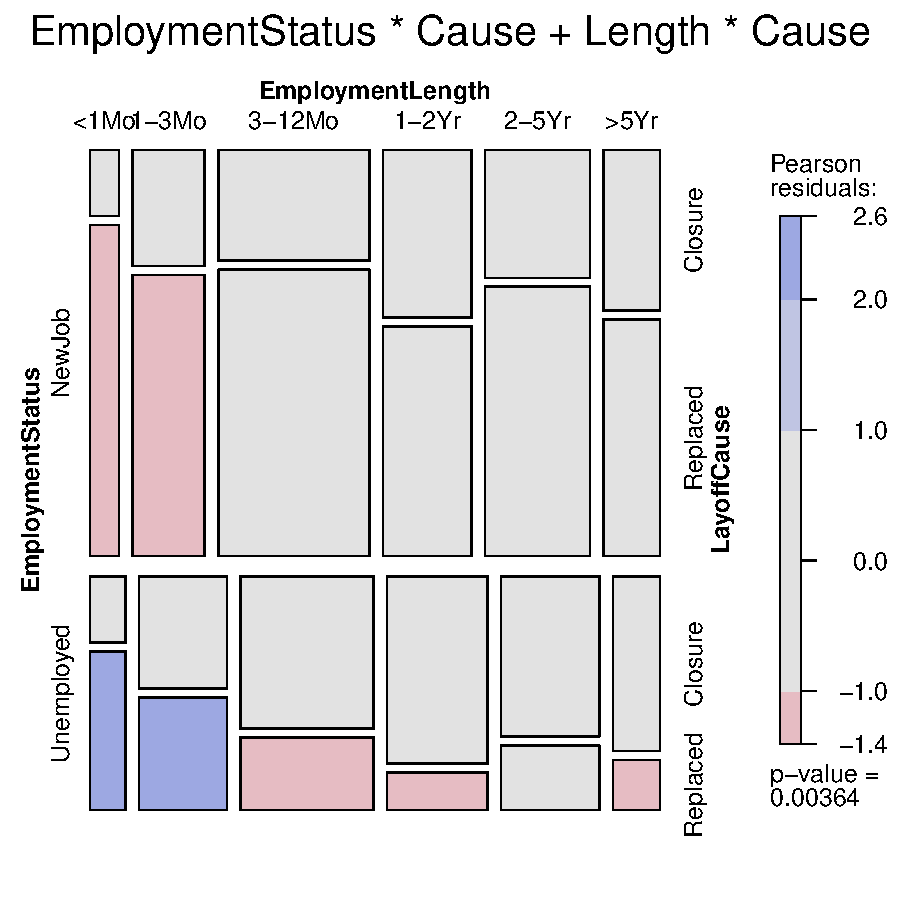
\includegraphics[width=.6\textwidth]{ch05/fig/employ-mos2-1} }

\caption[Mosaic display for the employment status data, fitting the model of conditional independence]{Mosaic display for the employment status data, fitting the model of conditional independence, [AC][BC].\label{fig:employ-mos2}}
\end{figure}


\end{knitrout}

To explain this result better, we can fit separate models for the \emph{partial}
relationship between \code{EmploymentStatus} and \code{EmploymentLength}
for the two levels of \code{LayoffCause}. In \R, with the \data{Employment} data
as in table form, this is easily done using \func{apply} over the
\code{LayoffCause} margin, giving a list containing the two \func{loglm} models.

\begin{knitrout}
\definecolor{shadecolor}{rgb}{1, 0.961, 0.933}\color{fgcolor}\begin{kframe}
\begin{alltt}
\hlstd{> }\hlstd{mods.list} \hlkwb{<-} \hlkwd{apply}\hlstd{(Employment,} \hlstr{"LayoffCause"}\hlstd{,}
\hlstd{+ }                   \hlkwa{function}\hlstd{(}\hlkwc{x}\hlstd{)} \hlkwd{loglm}\hlstd{(}\hlopt{~} \hlstd{EmploymentStatus} \hlopt{+} \hlstd{EmploymentLength,} \hlkwc{data} \hlstd{= x))}
\hlstd{> }\hlstd{mods.list}
\end{alltt}
\begin{verbatim}
$Closure
Call:
loglm(formula = ~EmploymentStatus + EmploymentLength, data = x)

Statistics:
                    X^2 df P(> X^2)
Likelihood Ratio 1.4786  5  0.91553
Pearson          1.4835  5  0.91497

$Replaced
Call:
loglm(formula = ~EmploymentStatus + EmploymentLength, data = x)

Statistics:
                    X^2 df   P(> X^2)
Likelihood Ratio 23.151  5 0.00031578
Pearson          24.589  5 0.00016727
\end{verbatim}
\end{kframe}
\end{knitrout}
Extracting the model fit statistics for these partial models and adding the
fit statistics for the overall model of conditional independence, \LLM{AC,BC}
gives the table below, illustrating the additive property of \GSQ, (\eqref{eq:partial1})
and \chisq.
\medskip
\begin{center}
\begin{tabular}{lrrr}
 \hline
 Model   &                 df   &  \GSQ   & \chisq \\
 \hline
 $A \perp B \given C_1$  &  5   &   1.49  &  1.48 \\
 $A \perp B \given C_2$  &  5   &  23.15  & 24.59 \\
 \hline
 $A \perp B \given C$    &  10  &  24.63  & 26.07 \\
\end{tabular}
\end{center}

One simple way to visualize these results is to call \func{mosaic}  separately
for each of the layers corresponding to \code{LayoffCause}.  The result is shown
in \figref{fig:employ-mos3}.

\begin{knitrout}
\definecolor{shadecolor}{rgb}{1, 0.961, 0.933}\color{fgcolor}\begin{kframe}
\begin{alltt}
\hlstd{> }\hlkwd{mosaic}\hlstd{(Employment[,,}\hlstr{"Closure"}\hlstd{],} \hlkwc{shade} \hlstd{=} \hlnum{TRUE}\hlstd{,} \hlkwc{gp_args} \hlstd{=} \hlkwd{list}\hlstd{(}\hlkwc{interpolate} \hlstd{=} \hlnum{1} \hlopt{:} \hlnum{4}\hlstd{),}
\hlstd{+ }       \hlkwc{margin} \hlstd{=} \hlkwd{c}\hlstd{(}\hlkwc{right} \hlstd{=} \hlnum{1}\hlstd{),} \hlkwc{main} \hlstd{=} \hlstr{"Layoff: Closure"}\hlstd{)}
\hlstd{> }\hlkwd{mosaic}\hlstd{(Employment[,,}\hlstr{"Replaced"}\hlstd{],} \hlkwc{shade} \hlstd{=} \hlnum{TRUE}\hlstd{,} \hlkwc{gp_args} \hlstd{=} \hlkwd{list}\hlstd{(}\hlkwc{interpolate} \hlstd{=} \hlnum{1} \hlopt{:} \hlnum{4}\hlstd{),}
\hlstd{+ }       \hlkwc{margin} \hlstd{=} \hlkwd{c}\hlstd{(}\hlkwc{right} \hlstd{=} \hlnum{1}\hlstd{),} \hlkwc{main} \hlstd{=} \hlstr{"Layoff: Replaced"}\hlstd{)}
\end{alltt}
\end{kframe}\begin{figure}[!htbp]

\centerline{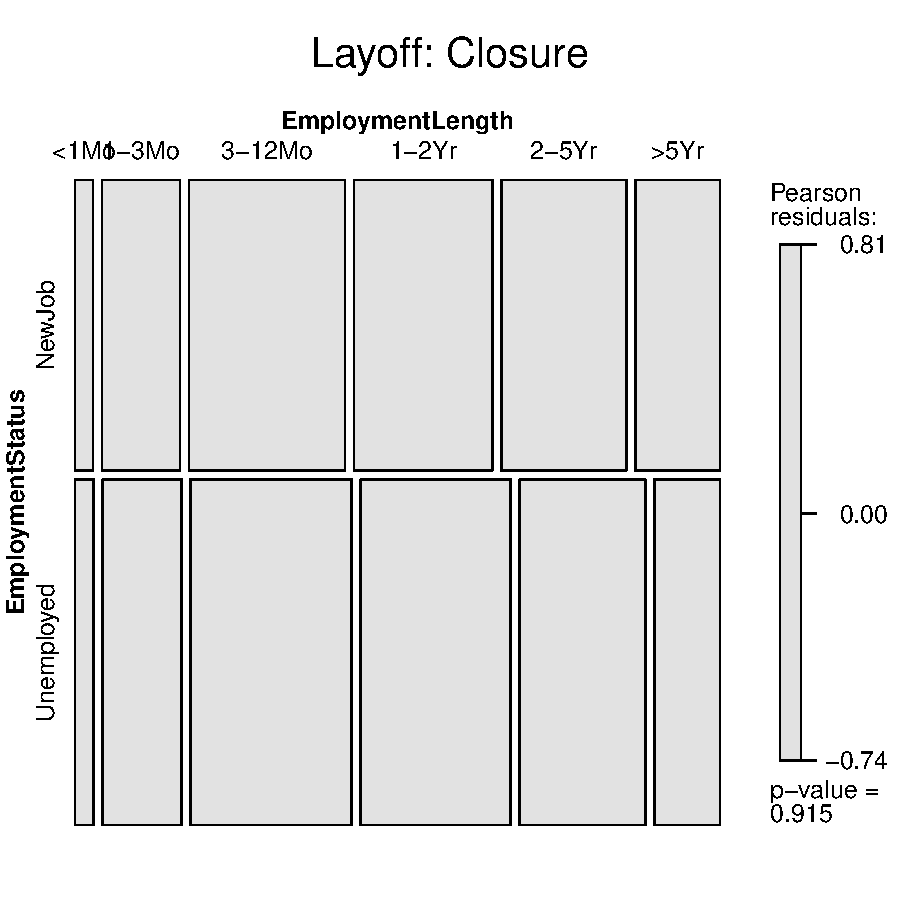
\includegraphics[width=.49\textwidth]{ch05/fig/employ-mos3-1} 
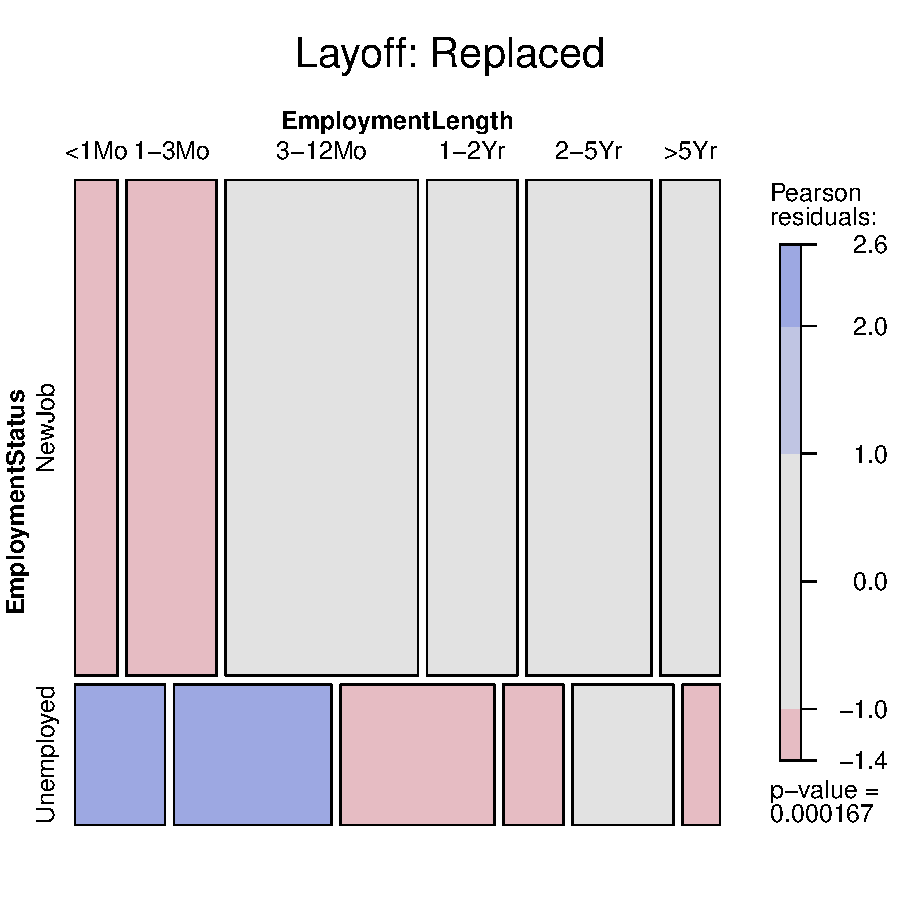
\includegraphics[width=.49\textwidth]{ch05/fig/employ-mos3-2} }

\caption[Mosaic displays for the employment status data, with separate panels for cause of layoff]{Mosaic displays for the employment status data, with separate panels for cause of layoff.\label{fig:employ-mos3}}
\end{figure}


\end{knitrout}
The simple summary from this example is that for workers laid off due to closure of
their company, length of previous employment is unrelated to whether or not they
are re-employed.  However, for workers who were replaced,
there is a systematic pattern:
those who had been employed for three months or less
are likely to remain unemployed, while those
with longer job tenure are somewhat more likely to have found a new job.
\end{Example}

The statistical methods and \R techniques described above for three-way tables
extend naturally to higher-way tables, as can be seen in the next example.

\begin{Example}[punish]{Corporal punishment data}
Here we use the \data{Punishment} data from \pkg{vcd}
which contains the results of
a study by the Gallup Institute in Denmark in 1979 about the attitude of a random sample of 1,456 persons towards corporal punishment of children \citep[pp. 207-208]{Andersen:91}.
As shown below, this data set is a frequency data frame representing a
$2 \times 2 \times 3 \times 3$ table, with table variables
\begin{seriate}
 \item \code{attitude} toward use of corporal punishment (approve of ``moderate'' use or ``no'' approval)
 \item \code{memory} of whether the respondent had experienced corporal punishment as a child (yes/no);
 \item \code{education} level of respondent (elementary, secondary, high);
 \item \code{age} category of respondent.
\end{seriate}
\begin{knitrout}\footnotesize
\definecolor{shadecolor}{rgb}{1, 0.961, 0.933}\color{fgcolor}\begin{kframe}
\begin{alltt}
\hlstd{> }\hlkwd{data}\hlstd{(}\hlstr{"Punishment"}\hlstd{,} \hlkwc{package} \hlstd{=} \hlstr{"vcd"}\hlstd{)}
\hlstd{> }\hlkwd{str}\hlstd{(Punishment)}
\end{alltt}
\begin{verbatim}
'data.frame':	36 obs. of  5 variables:
 $ Freq     : num  1 3 20 2 8 4 2 6 1 26 ...
 $ attitude : Factor w/ 2 levels "no","moderate": 1 1 1 1 1 1 1 1 1 1 ...
 $ memory   : Factor w/ 2 levels "yes","no": 1 1 1 1 1 1 1 1 1 2 ...
 $ education: Factor w/ 3 levels "elementary","secondary",..: 1 1 1 2 2 2 3 3 3 1 ...
 $ age      : Factor w/ 3 levels "15-24","25-39",..: 1 2 3 1 2 3 1 2 3 1 ...
\end{verbatim}
\end{kframe}
\end{knitrout}
Of main interest here is the association between attitude toward corporal punishment as an adult ($A$)
and memory of corporal punishment as a child ($B$),
controlling for age ($C$) and education ($D$); that is, the model $A \perp B \given (C,D)$,
or \LLM{ACD,BCD} in shorthand notation.

As noted above, this conditional independence
hypothesis can be decomposed into the $3 \times 3$ partial tests of
$A \perp B \given (C_k,D_\ell)$.

These tests and the associated graphics are somewhat easier to carry out with the data
in table form (\code{pun}) constructed below.  While we're at it, we recode the
variable names and factor levels for nicer graphical displays.
\begin{knitrout}
\definecolor{shadecolor}{rgb}{1, 0.961, 0.933}\color{fgcolor}\begin{kframe}
\begin{alltt}
\hlstd{> }\hlstd{pun} \hlkwb{<-} \hlkwd{xtabs}\hlstd{(Freq} \hlopt{~} \hlstd{memory} \hlopt{+} \hlstd{attitude} \hlopt{+} \hlstd{age} \hlopt{+} \hlstd{education,} \hlkwc{data} \hlstd{= Punishment)}
\hlstd{> }\hlkwd{dimnames}\hlstd{(pun)} \hlkwb{<-} \hlkwd{list}\hlstd{(}
\hlstd{+ }  \hlkwc{Memory} \hlstd{=} \hlkwd{c}\hlstd{(}\hlstr{"yes"}\hlstd{,} \hlstr{"no"}\hlstd{),}
\hlstd{+ }  \hlkwc{Attitude} \hlstd{=} \hlkwd{c}\hlstd{(}\hlstr{"no"}\hlstd{,} \hlstr{"moderate"}\hlstd{),}
\hlstd{+ }  \hlkwc{Age} \hlstd{=} \hlkwd{c}\hlstd{(}\hlstr{"15-24"}\hlstd{,} \hlstr{"25-39"}\hlstd{,} \hlstr{"40+"}\hlstd{),}
\hlstd{+ }  \hlkwc{Education} \hlstd{=} \hlkwd{c}\hlstd{(}\hlstr{"Elementary"}\hlstd{,} \hlstr{"Secondary"}\hlstd{,} \hlstr{"High"}\hlstd{))}
\end{alltt}
\end{kframe}
\end{knitrout}

Then, the overall test of conditional independence can be carried using \func{loglm} out as
\begin{knitrout}
\definecolor{shadecolor}{rgb}{1, 0.961, 0.933}\color{fgcolor}\begin{kframe}
\begin{alltt}
\hlstd{> }\hlstd{(mod.cond} \hlkwb{<-} \hlkwd{loglm}\hlstd{(}\hlopt{~} \hlstd{Memory} \hlopt{*} \hlstd{Age} \hlopt{*} \hlstd{Education} \hlopt{+} \hlstd{Attitude} \hlopt{*} \hlstd{Age} \hlopt{*} \hlstd{Education,}
\hlstd{+ }                   \hlkwc{data} \hlstd{= pun))}
\end{alltt}
\begin{verbatim}
Call:
loglm(formula = ~Memory * Age * Education + Attitude * Age * 
    Education, data = pun)

Statistics:
                    X^2 df   P(> X^2)
Likelihood Ratio 39.679  9 8.6851e-06
Pearson          34.604  9 6.9964e-05
\end{verbatim}
\end{kframe}
\end{knitrout}
Alternatively, \func{coindep\_test} in \pkg{vcd}
provides tests of conditional independence of two variables in a contingency table by simulation from the marginal permutation
distribution of the input table.  The version reporting a Pearson \chisq
statistic is given by
\begin{knitrout}
\definecolor{shadecolor}{rgb}{1, 0.961, 0.933}\color{fgcolor}\begin{kframe}
\begin{alltt}
\hlstd{> }\hlkwd{set.seed}\hlstd{(}\hlnum{1071}\hlstd{)}
\hlstd{> }\hlkwd{coindep_test}\hlstd{(pun,} \hlkwc{margin} \hlstd{=} \hlkwd{c}\hlstd{(}\hlstr{"Age"}\hlstd{,} \hlstr{"Education"}\hlstd{),}
\hlstd{+ }             \hlkwc{indepfun} \hlstd{=} \hlkwa{function}\hlstd{(}\hlkwc{x}\hlstd{)} \hlkwd{sum}\hlstd{(x} \hlopt{^} \hlnum{2}\hlstd{),} \hlkwc{aggfun} \hlstd{= sum)}
\end{alltt}
\begin{verbatim}

	Permutation test for conditional independence

data:  pun
f(x) = 34.604, p-value < 2.2e-16
\end{verbatim}
\end{kframe}
\end{knitrout}
These tests all show substantial association between attitude and memory of corporal
punishment.  How can we understand and explain this?

As in \exref{ex:employ}, we can partition the overall \GSQ or \chisq
to show the contributions to this association
from the combinations of age and education.  The call to \func{apply} below
returns a $3 \times 3$ matrix, each of whose elements is the list of results
returned by \func{loglm}.  The Pearson \chisq statistics for each subtable
can be extracted using \func{sapply} as shown below.

\begin{knitrout}
\definecolor{shadecolor}{rgb}{1, 0.961, 0.933}\color{fgcolor}\begin{kframe}
\begin{alltt}
\hlstd{> }\hlstd{mods.list} \hlkwb{<-} \hlkwd{apply}\hlstd{(pun,} \hlkwd{c}\hlstd{(}\hlstr{"Age"}\hlstd{,} \hlstr{"Education"}\hlstd{),}
\hlstd{+ }                   \hlkwa{function}\hlstd{(}\hlkwc{x}\hlstd{)} \hlkwd{loglm}\hlstd{(}\hlopt{~} \hlstd{Memory} \hlopt{+} \hlstd{Attitude,} \hlkwc{data} \hlstd{= x))}
\hlstd{> }\hlstd{XSQ} \hlkwb{<-} \hlkwd{matrix}\hlstd{(}\hlkwd{sapply}\hlstd{(mods.list,} \hlkwa{function}\hlstd{(}\hlkwc{x}\hlstd{)x}\hlopt{$}\hlstd{pearson),} \hlnum{3}\hlstd{,} \hlnum{3}\hlstd{)}
\hlstd{> }\hlkwd{dimnames}\hlstd{(XSQ)} \hlkwb{<-} \hlkwd{dimnames}\hlstd{(mods.list)}
\hlstd{> }\hlkwd{addmargins}\hlstd{(XSQ)}
\end{alltt}
\begin{verbatim}
       Education
Age     Elementary Secondary     High     Sum
  15-24     3.5907  0.078782 0.091429  3.7609
  25-39     8.5844  0.934669 0.480000  9.9990
  40+      11.6256  6.094854 3.123714 20.8442
  Sum      23.8006  7.108305 3.695143 34.6041
\end{verbatim}
\end{kframe}
\end{knitrout}
One visual analog of this table of \chisq statistics is a \func{cotabplot} of the
(conditional) association of attitude and memory over the age and education cells,
shown in \figref{fig:punish-cond1}.  \func{cotabplot} is very general, allowing
a variety of functions of the residuals to be used for shading
\citep{Zeileis-etal:2007}.
Here we use
the (Pearson) sum of squares statistic, $\sum_{k, \ell} \chisq_{k,\ell}$.
\begin{knitrout}
\definecolor{shadecolor}{rgb}{1, 0.961, 0.933}\color{fgcolor}\begin{kframe}
\begin{alltt}
\hlstd{> }\hlkwd{set.seed}\hlstd{(}\hlnum{1071}\hlstd{)}
\hlstd{> }\hlstd{pun_cotab} \hlkwb{<-} \hlkwd{cotab_coindep}\hlstd{(pun,} \hlkwc{condvars} \hlstd{=} \hlnum{3} \hlopt{:} \hlnum{4}\hlstd{,} \hlkwc{type} \hlstd{=} \hlstr{"mosaic"}\hlstd{,}
\hlstd{+ }  \hlkwc{varnames} \hlstd{=} \hlnum{FALSE}\hlstd{,} \hlkwc{margins} \hlstd{=} \hlkwd{c}\hlstd{(}\hlnum{2}\hlstd{,} \hlnum{1}\hlstd{,} \hlnum{1}\hlstd{,} \hlnum{2}\hlstd{),}
\hlstd{+ }  \hlkwc{test} \hlstd{=} \hlstr{"sumchisq"}\hlstd{,} \hlkwc{interpolate} \hlstd{=} \hlnum{1} \hlopt{:} \hlnum{2}\hlstd{)}
\hlstd{> }\hlkwd{cotabplot}\hlstd{(}\hlopt{~} \hlstd{Memory} \hlopt{+} \hlstd{Attitude} \hlopt{|} \hlstd{Age} \hlopt{+} \hlstd{Education,} \hlkwc{data} \hlstd{=}
\hlstd{+ }            \hlstd{pun,} \hlkwc{panel} \hlstd{= pun_cotab)}
\end{alltt}
\end{kframe}\begin{figure}[!htb]

\centerline{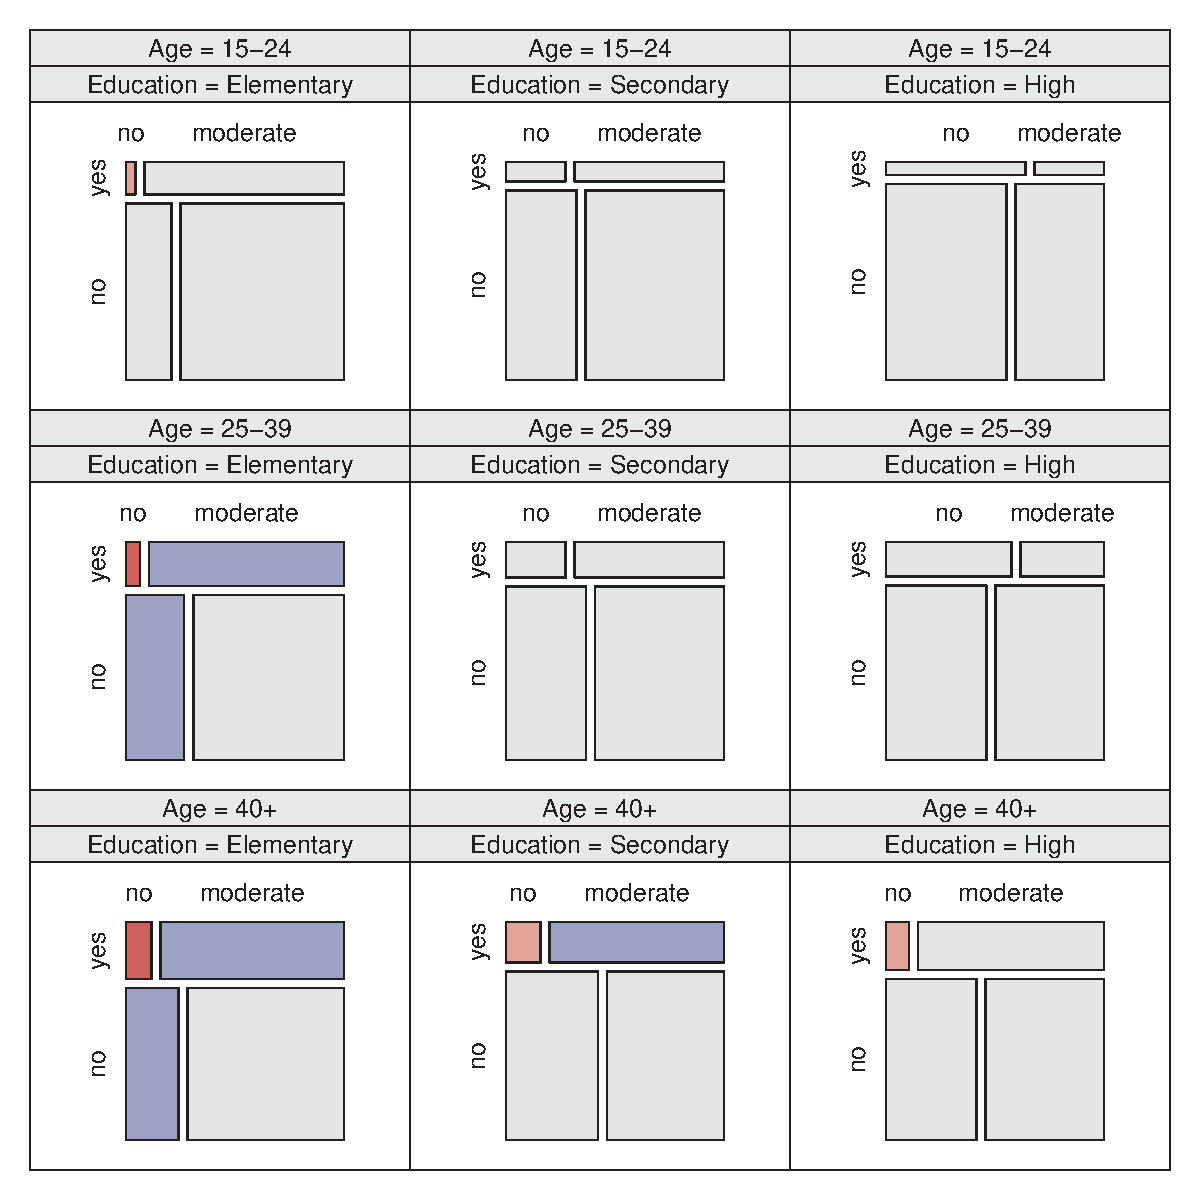
\includegraphics[width=.95\textwidth]{ch05/fig/punish-cond1-1} }

\caption[Conditional mosaic plot of the Punishment data for the model of conditional independence of attitude and memory, given age and education]{Conditional mosaic plot of the Punishment data for the model of conditional independence of attitude and memory, given age and education. Shading of tiles is based on the sum of squares statistic.\label{fig:punish-cond1}}
\end{figure}


\end{knitrout}

Alternatively, the pattern of conditional association can be shown somewhat more directly
in a conditional mosaic plot (\figref{fig:punish-cond2}), using the same model formula to condition on
age and education. This simply organizes the display to split on the conditioning
variables first, with larger spacings.
\begin{knitrout}
\definecolor{shadecolor}{rgb}{1, 0.961, 0.933}\color{fgcolor}\begin{kframe}
\begin{alltt}
\hlstd{> }\hlkwd{mosaic}\hlstd{(}\hlopt{~} \hlstd{Memory} \hlopt{+} \hlstd{Attitude} \hlopt{|} \hlstd{Age} \hlopt{+} \hlstd{Education,} \hlkwc{data} \hlstd{= pun,}
\hlstd{+ }       \hlkwc{shade} \hlstd{=} \hlnum{TRUE}\hlstd{,} \hlkwc{gp_args} \hlstd{=} \hlkwd{list}\hlstd{(}\hlkwc{interpolate} \hlstd{=} \hlnum{1} \hlopt{:} \hlnum{4}\hlstd{))}
\end{alltt}
\end{kframe}\begin{figure}[!htb]

\centerline{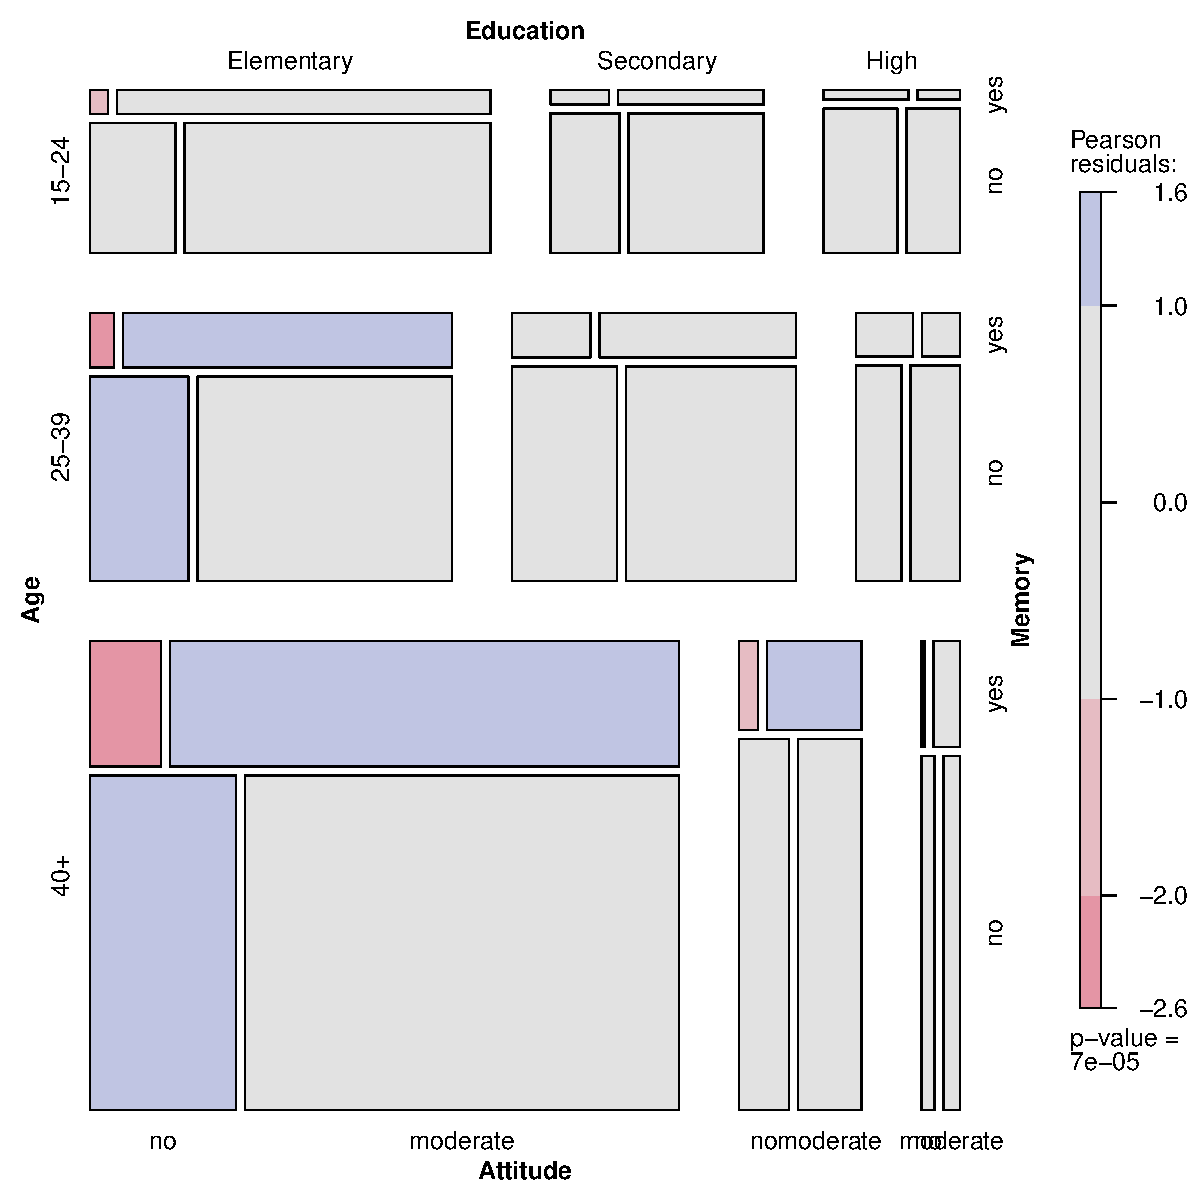
\includegraphics[width=.8\textwidth]{ch05/fig/punish-cond2-1} }

\caption[Conditional mosaic plot of the Punishment data for the model of conditional independence of attitude and memory, given age and education]{Conditional mosaic plot of the Punishment data for the model of conditional independence of attitude and memory, given age and education. This plot explicitly shows the total frequencies in the cells of age and education by the areas of the main blocks for these variables.\label{fig:punish-cond2}}
\end{figure}


\end{knitrout}
Both \figref{fig:punish-cond1} and \figref{fig:punish-cond2} reveal that the
association between attitude and memory becomes stronger with increasing age
among those with the lowest education (first column).
Among those in the highest age group (bottom row), the strength of association \emph{decreases}
with increasing education.  These two displays differ in that in the
\func{cotabplot} of \figref{fig:punish-cond1} the marginal frequencies of
age and education are not shown, whereas in the \func{mosaic} of \figref{fig:punish-cond2}
they determine the relative sizes of the tiles for the combinations of age and education.

The divide-and-conquer strategy of partial association using statistical tests and
visual displays now provides a simple, coherent explanation for this table:
memory of experienced violence as a child tends to engender a more favorable
attitude toward corporal punishment as an adult, but this association varies
directly with both age and education.
\end{Example}


\section{Mosaic matrices for categorical data}\label{sec:mosmat}

One reason for the wide usefulness of graphs of quantitative data
has been the
development of effective, general techniques for dealing with high-dimensional \Dsets.
The \term{scatterplot matrix}
%(\SSSGref{8.3.2})
shows all pairwise (marginal) views of a set of variables
in a coherent display, whose design goal is to show the interdependence
among the collection of variables as a whole.
It combines multiple views of the data
into a single display which allows detection of patterns which could
not readily be discerned from a series of separate graphs.
In effect, a multivariate \Dset in $p$ dimensions (variables) is shown as
a collection of $p (p-1)$ two-dimensional \scats, each of which is
the projection of the cloud of points on two of the variable axes.
These ideas can be readily extended to categorical data.

A \mway \ctab of $p$ categorical variables,
$A, B, C,\dots$, contains the interdependence among the collection
of variables as a whole.  The saturated \loglin model, $[A B C\dots]$
fits this interdependence perfectly, but is often too complex to describe
or understand.

By summing the table over all variables except two,
$A$ and $B$, say, we obtain a two-variable (marginal) table, showing the
bivariate relationship between $A$ and $B$, which is also a projection
of the $p$-variable relation into the space of two (categorical) variables.
If we do this for all $p (p-1)$ unordered pairs of categorical variables
and display each two-variable table as a mosaic,  we have a categorical
analog of the \scatmat, called a
\term{mosaic matrix}.
Like the \scatmat, the mosaic matrix can accommodate any number of
variables in principle, but in practice is limited by the resolution
of our display to three or four variables.

In \R, the main implementation of this idea is in the generic function
\func{pairs}.  The \Rpackage{vcd} extends this to
mosaic matrices with methods
for \class{table} and \class{structable} objects.
The \Rpackage{gpairs} provides a \term{generalized pairs plot},
with appropriate graphics for a mixture of quantitative and categorical
variables.

\begin{Example}[bartlett]{Bartlett data on plum root cuttings}
The simplest example of what you can see in a mosaic matrix is
provided by the $2 \times 2 \times 2$ table
used by \citet{Bartlett:35}
to illustrate a method for testing for no three-way interaction in a contingency table
(hypothesis $H_4$ in \tabref{tab:hyp3way}).

The data set \data{Bartlett} in \pkg{vcdExtra}
gives the result of an agricultural experiment to
investigate the survival of plum root cuttings (\var{Alive})
in relation to two factors: \var{Time} of planting and the \var{Length} of the cutting.
In this experiment, 240 cuttings were planted for each of the $2 \times 2$ combinations of these factors, and their survival (Alive, Dead) was later recorded.

\begin{knitrout}
\definecolor{shadecolor}{rgb}{1, 0.961, 0.933}\color{fgcolor}\begin{kframe}
\begin{alltt}
\hlstd{> }\hlkwd{pairs}\hlstd{(Bartlett,} \hlkwc{gp} \hlstd{= shading_Friendly)}
\end{alltt}
\end{kframe}\begin{figure}[!htb]

\centerline{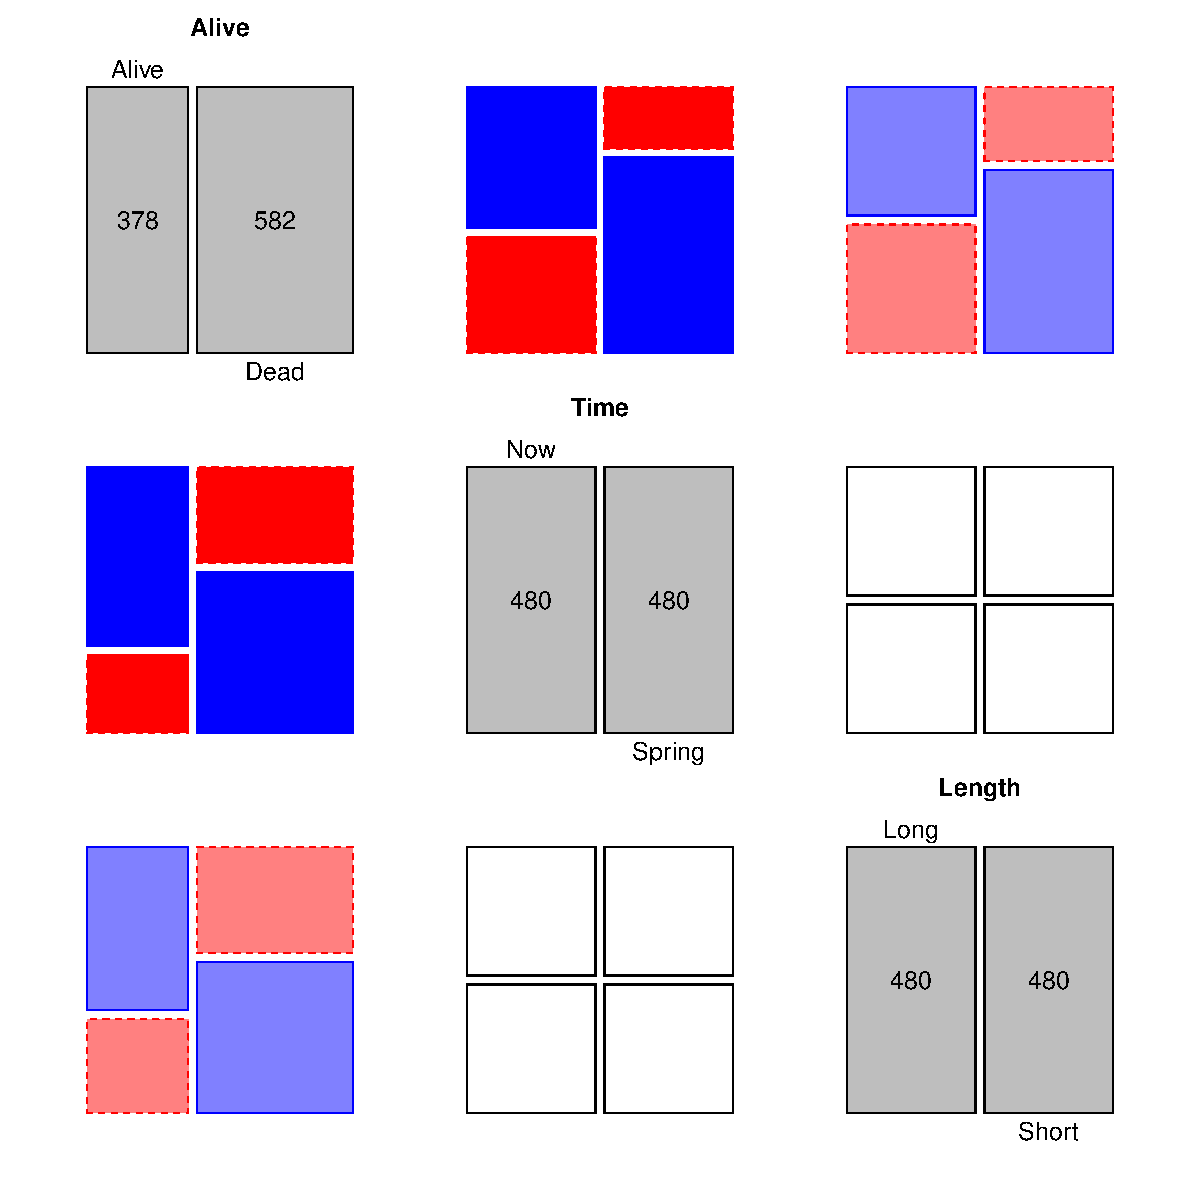
\includegraphics[width=.8\textwidth]{ch05/fig/bartlett-pairs-1} }

\caption[Mosaic pairs plot for the Bartlett data]{Mosaic pairs plot for the Bartlett data. Each panel shows the bivariate marginal relation between the row and column variables.\label{fig:bartlett-pairs}}
\end{figure}


\end{knitrout}
The mosaic matrix for these data, showing all twoway marginal relations, is shown
in \figref{fig:bartlett-pairs}.
It can immediately be seen that \var{Time} and \var{Length} are independent
by the design of the experiment; we use \code{gp=shading\_Friendly} here to emphasize
this.

The top row and left column show the relation of survival to each of time of planting
and cutting length.  It is easily seen that greater survival is associated with
cuttings taken now (vs. spring) and those cut long (vs. short),
and the degree of association is stronger for planting time than for cutting length.
\end{Example}

\begin{Example}[marital2]{Marital status and pre- and extramarital sex}
In \exref{ex:marital1} we examined a series of models relating marital
status to reported premarital and extramarital sexual activity and gender in the
\data{PreSex} data.
\figref{fig:marital-pairs} shows the mosaic matrix for these data.
The diagonal panels show the labels for the category levels as well as
the one-way marginal totals.

\begin{knitrout}
\definecolor{shadecolor}{rgb}{1, 0.961, 0.933}\color{fgcolor}\begin{kframe}
\begin{alltt}
\hlstd{> }\hlkwd{data}\hlstd{(}\hlstr{"PreSex"}\hlstd{,} \hlkwc{package} \hlstd{=} \hlstr{"vcd"}\hlstd{)}
\hlstd{> }\hlkwd{pairs}\hlstd{(PreSex,} \hlkwc{gp} \hlstd{= shading_Friendly,} \hlkwc{gp_args} \hlstd{=} \hlkwd{list}\hlstd{(}\hlkwc{interpolate} \hlstd{=} \hlnum{1} \hlopt{:} \hlnum{4}\hlstd{),} \hlkwc{space} \hlstd{=} \hlnum{0.25}\hlstd{)}
\end{alltt}
\end{kframe}\begin{figure}[!htb]

\centerline{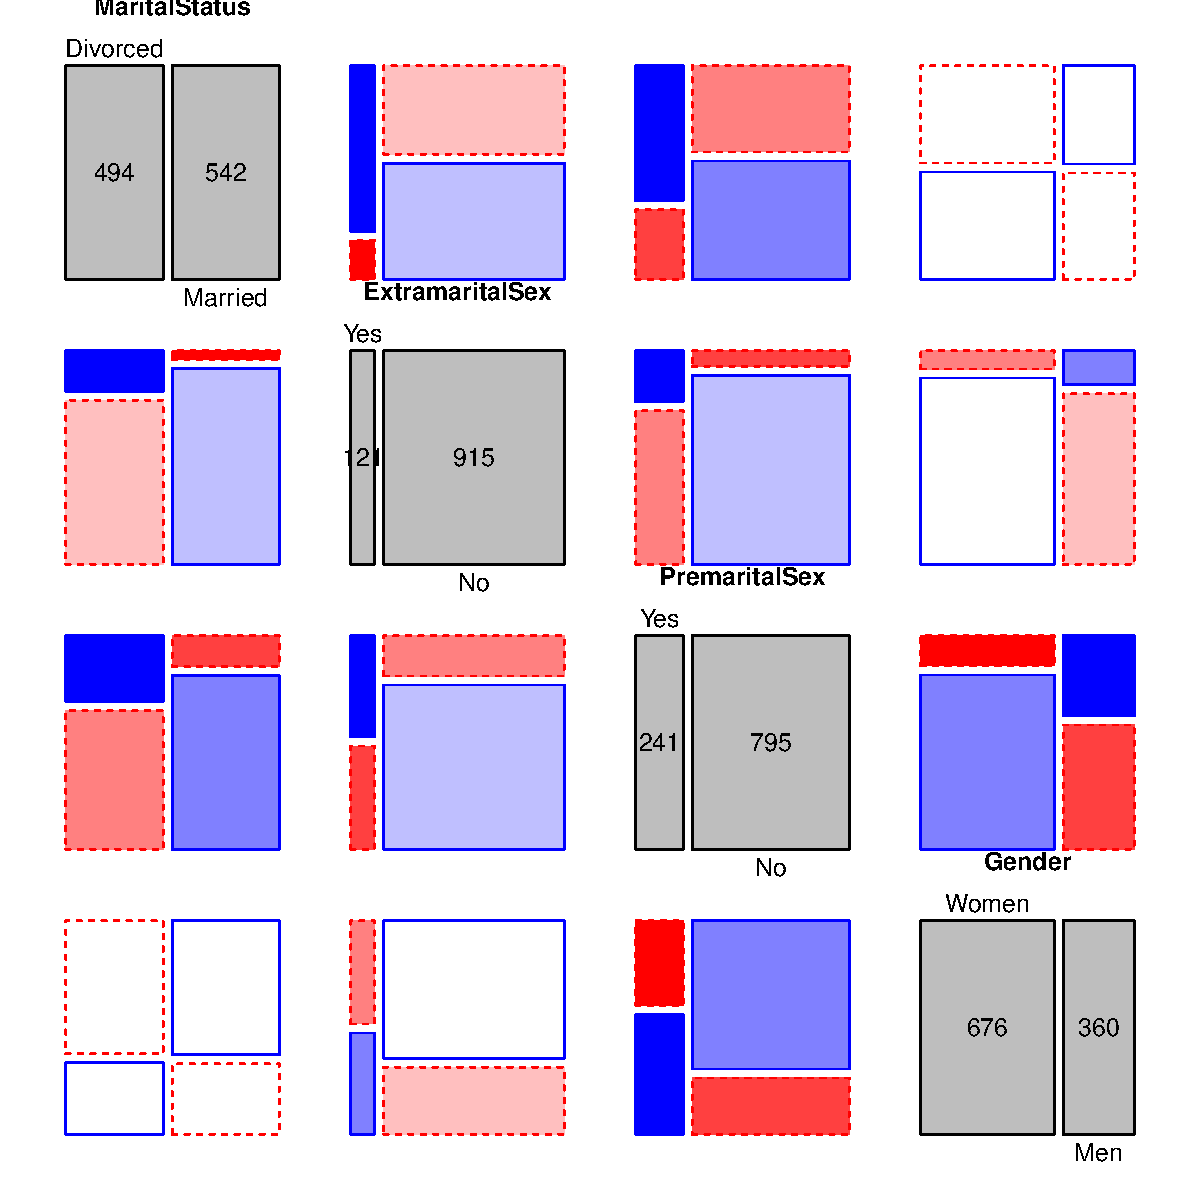
\includegraphics[width=.8\textwidth]{ch05/fig/marital-pairs-1} }

\caption[Mosaic pairs plot for the PreSex data]{Mosaic pairs plot for the PreSex data. Each panel shows the bivariate marginal relation between the row and column variables.\label{fig:marital-pairs}}
\end{figure}


\end{knitrout}
If we view gender, premarital sex and extramarital sex as explanatory,
and marital status (Divorced vs.\  still Married) as the response,
then the mosaics in row 1 (and in column 1)%
%
\footnote{Rows and columns in a mosaic matrix are identified
as in a table or numerical matrix, with row 1, column 1 in the upper left corner.}
%
shows how marital status
depends on each predictor marginally.
The remaining panels show the relations within the set of explanatory
variables.

Thus, we see in row 1, column 4, that marital status is independent
of gender (all residuals equal zero, here), by design of the data
collection.  In the (1, 3) panel, we see that reported premarital sex
is more often followed by divorce, while non-report is more prevalent
among those still married.  The (1, 2) panel shows a similar,
but stronger relation between extramarital sex and marriage stability.  These
effects pertain to the associations of P and E with marital status (M)---%
the terms [PM] and [EM] in the \loglin model.  We saw earlier that
an interaction of P and E (the term [PEM]) is required to fully account for these data.  This effect is not displayed in \figref{fig:marital-pairs}.

Among the background variables (the \loglin term [GPE]), the (2, 3) panel shows a strong relation
between premarital sex and subsequent extramarital sex, while
the (2, 4) and (3, 4) panels show that men are far more likely to report
premarital sex than women in this sample, and also more likely to
report extramarital sex.

Even though the mosaic matrix shows only pairwise, bivariate associations,
it provides an integrated view of all of these together in a single display.

\end{Example}

\begin{Example}[berkeley4]{Berkeley admissions}
In \chref{ch:twoway} we examined the
relations among the variables Admit, Gender and Department in the Berkeley
admissions data (\exref{ex:berkeley1}, \exref{ex:berkeley2}, \exref{ex:berkeley3})
using fourfold displays
(\figref{fig:berk-fourfold3} and \figref{fig:berk-fourfold4})
and sieve diagrams (\figref{fig:berkeley-sieve}).
These displays showed either a marginal relation (e.g., Admit, Gender)
or the full three-way table.

In contrast, \figref{fig:berk-pairs1} shows all pairwise marginal
relations among these variables, produced using \func{pairs}.  Some additional
arguments are used to control the details of labels for the diagonal and off-diagonal panels.
\begin{knitrout}
\definecolor{shadecolor}{rgb}{1, 0.961, 0.933}\color{fgcolor}\begin{kframe}
\begin{alltt}
\hlstd{> }\hlstd{largs} \hlkwb{<-} \hlkwd{list}\hlstd{(}\hlkwc{labeling} \hlstd{=} \hlkwd{labeling_border}\hlstd{(}\hlkwc{varnames} \hlstd{=} \hlnum{FALSE}\hlstd{,}
\hlstd{+ }              \hlkwc{labels} \hlstd{=} \hlkwd{c}\hlstd{(T, T, F, T),} \hlkwc{alternate_labels} \hlstd{=} \hlnum{FALSE}\hlstd{))}
\hlstd{> }\hlstd{dargs} \hlkwb{<-} \hlkwd{list}\hlstd{(}\hlkwc{gp_varnames} \hlstd{=} \hlkwd{gpar}\hlstd{(}\hlkwc{fontsize} \hlstd{=} \hlnum{20}\hlstd{),} \hlkwc{offset_varnames} \hlstd{=} \hlopt{-}\hlnum{1}\hlstd{,}
\hlstd{+ }              \hlkwc{labeling} \hlstd{=} \hlkwd{labeling_border}\hlstd{(}\hlkwc{alternate_labels} \hlstd{=} \hlnum{FALSE}\hlstd{))}
\hlstd{> }\hlkwd{pairs}\hlstd{(UCBAdmissions,} \hlkwc{shade} \hlstd{=} \hlnum{TRUE}\hlstd{,} \hlkwc{space} \hlstd{=} \hlnum{0.25}\hlstd{,}
\hlstd{+ }      \hlkwc{diag_panel_args} \hlstd{= dargs,}
\hlstd{+ }      \hlkwc{upper_panel_args} \hlstd{= largs,} \hlkwc{lower_panel_args} \hlstd{= largs)}
\end{alltt}
\end{kframe}\begin{figure}[!htb]

\centerline{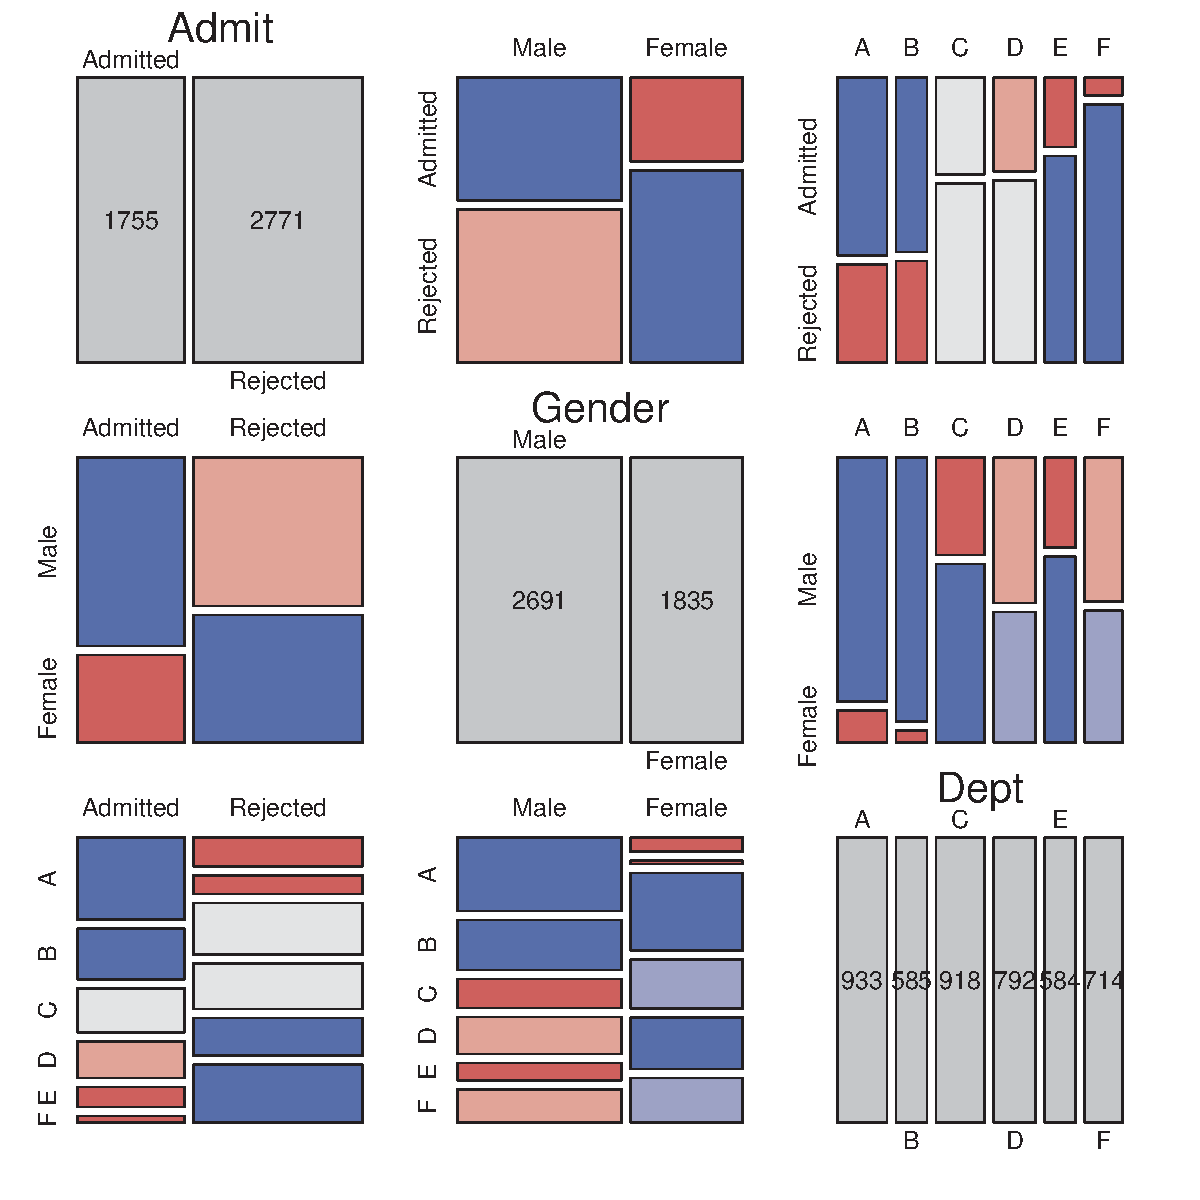
\includegraphics[width=.8\textwidth]{ch05/fig/berk-pairs1-1} }

\caption[Mosaic matrix of the UCBAdmissions data showing bivariate marginal relations]{Mosaic matrix of the UCBAdmissions data showing bivariate marginal relations\label{fig:berk-pairs1}}
\end{figure}


\end{knitrout}
The panel in row 2, column 1
shows that Admission and Gender are
strongly associated marginally, as we saw in \figref{fig:berk-fourfold3},
and overall, males are more often admitted.
The diagonally-opposite panel (row 1, column 2) shows the
same relation, splitting first by gender.%
\footnote{Note that this is different than just the transpose or interchange
of horizontal and vertical dimensions as in a \scatmat,
because the mosaic display splits the total frequency first by the horizontal
variable and then (conditionally) by the vertical variable.
The areas of all corresponding tiles are the same in each diagonally
opposite pair, however, as are the
residuals shown by color and shading.}

The panels in the third column (and third row)
provide the explanation for the paradoxical
result (see \figref{fig:berk-fourfold4}) that, within all but department A,
the likelihood of admission is equal for men and women,
yet, overall, there appears to be a bias in favor of admitting men
(see \figref{fig:fourfold3}).
The (1,3) and (3, 1) panels show
the marginal relation between Admission and Department, that is,
how admission rate varies across departments.
Departments A and B have the greatest
overall admission rate, departments E and F the least.
The (2, 3) and (3,2)
panels show how men and women apply differentially to
the various departments.
It can be seen that
men apply in much greater numbers to
departments A and B, with higher admission rates,
while women apply in greater numbers to
the departments C--F, with the lowest overall rate of admission.

\end{Example}

\subsection{Generalized mosaic matrices and pairs plots}\label{sec:condmat}

We need not show only the marginal relation between
each pair of variables in a mosaic matrix.
\citep{Friendly:99:EMD} describes the extension of this idea
to conditional, partial, and other views of a \ctab.

In \func{pairs.table}, different \term{panel functions} can be used
to specify what is displayed in the upper, lower and diagonal
panels.  For the off-diagonal panels, a \code{type} argument
can be used to plot mosaics showing various kinds of independence
relations:
\begin{description*}
  \item[\code{type="pairwise"}] Shows bivariate marginal relations, collapsed over all other variables.
  \item[\code{type="total"}] Shows mosaic plots for mutual independence.
  \item[\code{type="conditional"}] Shows mosaic plots for conditional independence given all other variables.
  \item[\code{type="joint"}] Shows mosaic plots for joint independence of all pairs of variables from the others.
\end{description*}

\begin{Example}[berkeley4b]{Berkeley admissions}
\figref{fig:berk-pairs2} shows the generalized mosaic matrix for the \data{UCBAdmissions}
data, using 3-way mosaics for all the off-diagonal cells.
The observed frequencies, of course, are the same in all these cells.
However, in the lower panels, the tiles are shaded according to models of
joint independence, while in the upper panels, they are shaded according to
models of mutual independence.
\begin{knitrout}
\definecolor{shadecolor}{rgb}{1, 0.961, 0.933}\color{fgcolor}\begin{kframe}
\begin{alltt}
\hlstd{> }\hlkwd{pairs}\hlstd{(UCBAdmissions,}
\hlstd{+ }      \hlkwc{lower_panel} \hlstd{=} \hlkwd{pairs_mosaic}\hlstd{(}\hlkwc{type} \hlstd{=} \hlstr{"joint"}\hlstd{,} \hlkwc{shade} \hlstd{=} \hlnum{TRUE}\hlstd{),}
\hlstd{+ }      \hlkwc{upper_panel} \hlstd{=} \hlkwd{pairs_mosaic}\hlstd{(}\hlkwc{type} \hlstd{=} \hlstr{"total"}\hlstd{,} \hlkwc{shade} \hlstd{=} \hlnum{TRUE}\hlstd{),}
\hlstd{+ }      \hlkwc{space}\hlstd{=}\hlnum{0.2}\hlstd{)}
\end{alltt}
\end{kframe}\begin{figure}[!htb]

\centerline{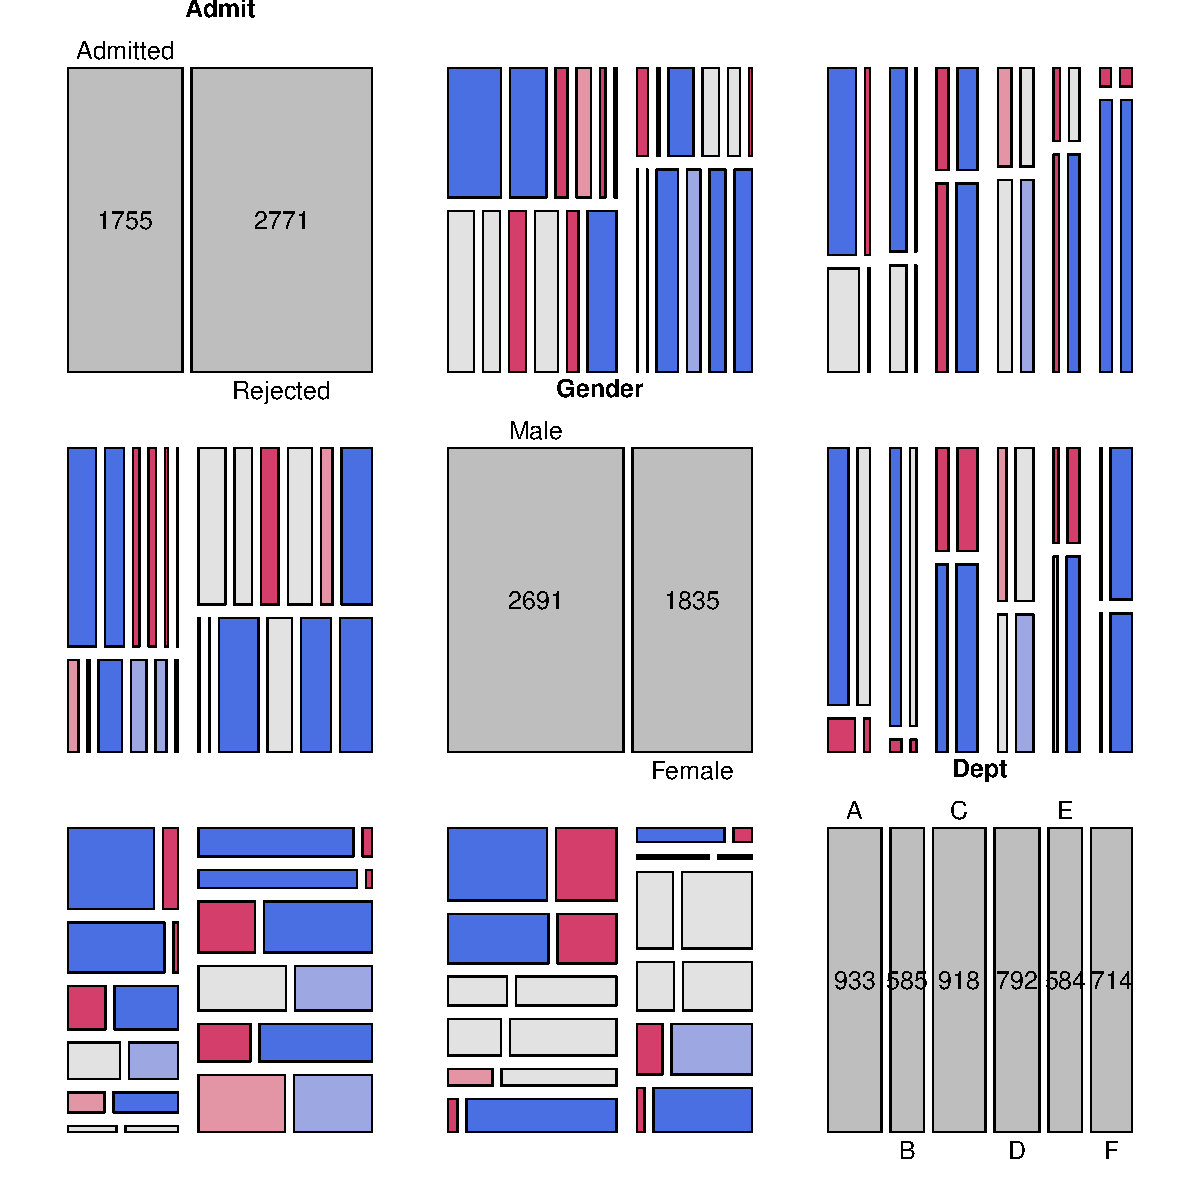
\includegraphics[width=.8\textwidth]{ch05/fig/berk-pairs2-1} }

\caption[Generalized mosaic matrix of the UCBAdmissions data]{Generalized mosaic matrix of the UCBAdmissions data. The above-diagonal plots fit models of joint independence; below-diagonal plots fit models of mutual independence.\label{fig:berk-pairs2}}
\end{figure}


\end{knitrout}
\TODO{Replace this with a figure using \code{type = "conditional"}, once we can get this to work.}

In this example, it is more useful to fit and display the models of conditional independence
for each pair of row, column variables given the remaining one, as shown in \figref{fig:berk-pairs3}.
\begin{knitrout}
\definecolor{shadecolor}{rgb}{1, 0.961, 0.933}\color{fgcolor}\begin{kframe}
\begin{alltt}
\hlstd{> }\hlkwd{pairs}\hlstd{(UCBAdmissions,}
\hlstd{+ }      \hlkwc{lower_panel} \hlstd{=} \hlkwd{pairs_mosaic}\hlstd{(}\hlkwc{type} \hlstd{=} \hlstr{"conditional"}\hlstd{,} \hlkwc{shade} \hlstd{=} \hlnum{TRUE}\hlstd{),}
\hlstd{+ }      \hlkwc{upper_panel} \hlstd{=} \hlkwd{pairs_mosaic}\hlstd{(}\hlkwc{type} \hlstd{=} \hlstr{"conditional"}\hlstd{,} \hlkwc{shade} \hlstd{=} \hlnum{TRUE}\hlstd{),}
\hlstd{+ }      \hlkwc{space} \hlstd{=} \hlnum{0.2}\hlstd{)}
\end{alltt}
\end{kframe}\begin{figure}[!htb]

\centerline{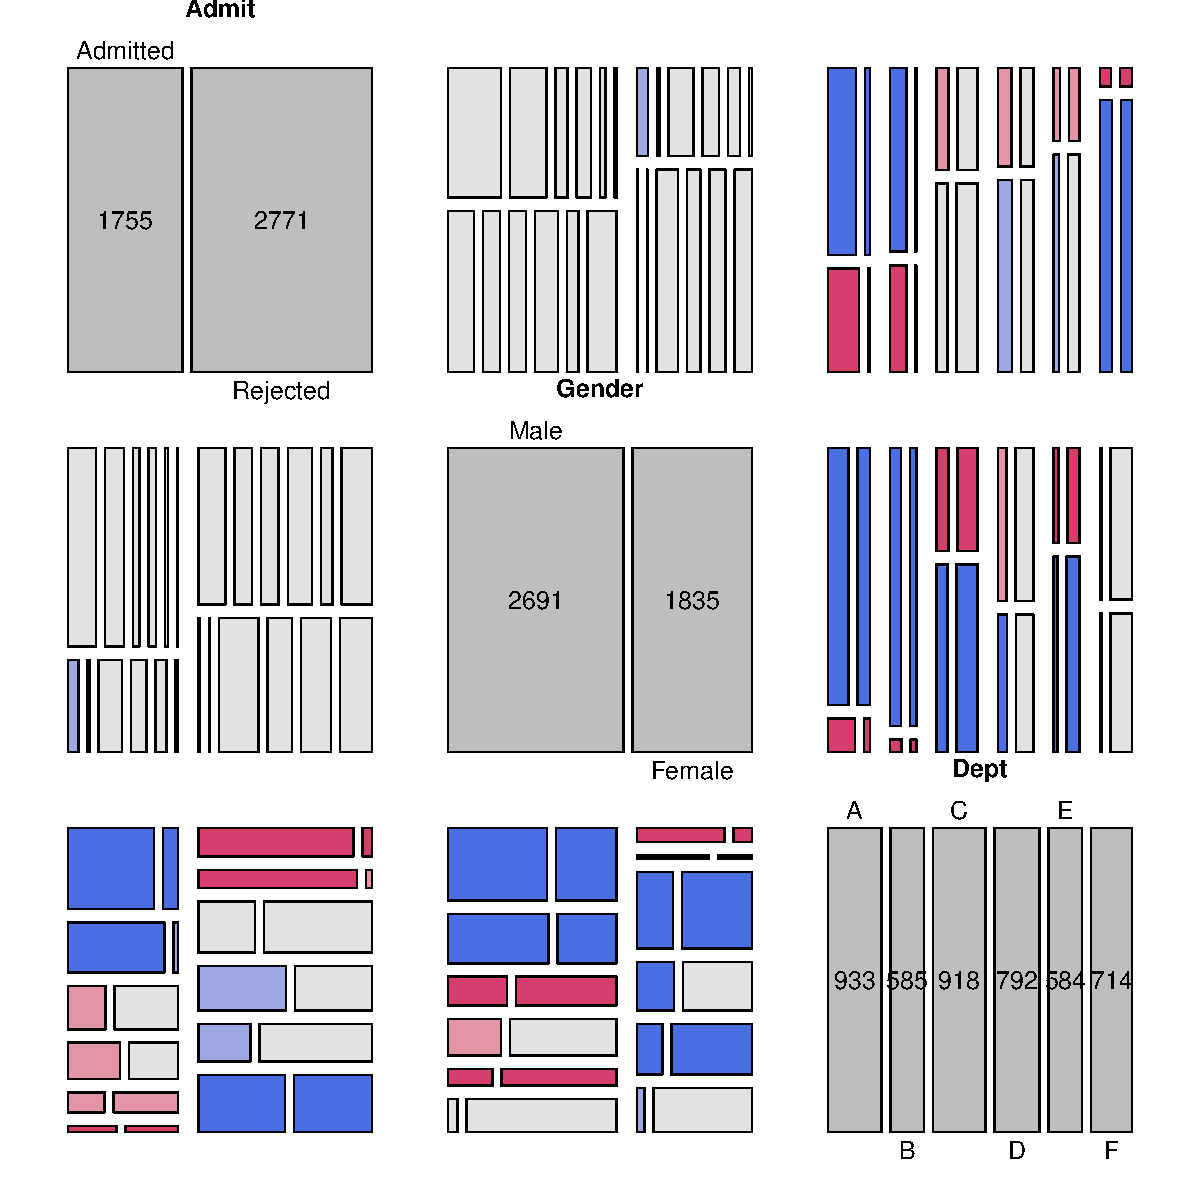
\includegraphics[width=.8\textwidth]{ch05/fig/berk-pairs3-1} }

\caption[Generalized mosaic matrix of the UCBAdmissions data]{Generalized mosaic matrix of the UCBAdmissions data. The above-diagonal plots fit models of joint independence; below-diagonal plots fit models of mutual independence.\label{fig:berk-pairs3}}
\end{figure}


\end{knitrout}
Thus, the shading in the (1,2) and (2,1) panels show the fit of the model
[Admit, Dept] [Gender, Dept],
which asserts that Admission and Gender are independent, given (controlling
for) Department.  Except for Department A, this model fits quite well,
again indicating lack of gender bias.
The (1,3) and (3,1) panels show the relation between admission and department
controlling for gender, highlighting the differential admission rates
across departments.
\TODO{This isn't quite right!}

\end{Example}

Beyond this, the framework of pairs plots can be further generalized to \emph{mixtures}
of quantitative and categorical variables, as first described in \citet{Friendly:03:apa}
and then in a wider context by \citet{Emerson-etal:2013,Friendly:2013:genpairs}.
The essential idea is to consider the combination of two variables, each of which can
be either categorical (\textbf{C}) or quantitative (\textbf{Q}), and various ways to \emph{render} that
combination in a graphical display:

\begin{description*}
  \item[\textbf{CC}:] mosaic display, sieve diagram, doubledecker plot, faceted or divided bar chart;
  \item[\textbf{CQ}:] side-by-side boxplots, stripplots, faceted histograms, aligned density plots;
  \item[\textbf{QQ}:] scatterplot, corrgram, data ellipses, etc.
\end{description*}
In \R some of these possibilities are provided in the \Rpackage{gpairs} (using \pkg{grid} graphics
and the \pkg{vcd} strucplot framework), and the \Rpackage{GGally}
(an extension to \pkg{ggplot2}).


\begin{Example}[arthritis-gpairs]{Arthritis treatment}
We illustrate these ideas with the \data{Arthritis} data using the
\Rpackage{gpairs} in \figref{fig:arth-gpairs}.
In this data, the variables \var{Treatment}, \var{Sex} and \var{Improved} are
categorical, and \var{Age} is quantitative.
The call to \func{gpairs} below reorders the variables to put the response variable
\var{Improved} in row 1, column 1. Various options can be passed to \func{mosaic}
using the \code{mosaic.pars} argument.
\begin{knitrout}
\definecolor{shadecolor}{rgb}{1, 0.961, 0.933}\color{fgcolor}\begin{kframe}
\begin{alltt}
\hlstd{> }\hlkwd{library}\hlstd{(gpairs)}
\end{alltt}


{\ttfamily\noindent\bfseries\color{errorcolor}{Error in library(gpairs): there is no package called 'gpairs'}}\begin{alltt}
\hlstd{> }\hlkwd{data}\hlstd{(}\hlstr{"Arthritis"}\hlstd{,} \hlkwc{package} \hlstd{=} \hlstr{"vcd"}\hlstd{)}
\hlstd{> }\hlkwd{gpairs}\hlstd{(Arthritis[,}\hlkwd{c}\hlstd{(}\hlnum{5}\hlstd{,} \hlnum{2}\hlstd{,} \hlnum{3}\hlstd{,} \hlnum{4}\hlstd{)],}
\hlstd{+ }       \hlkwc{diag.pars} \hlstd{=} \hlkwd{list}\hlstd{(}\hlkwc{fontsize} \hlstd{=} \hlnum{20}\hlstd{),}
\hlstd{+ }       \hlkwc{mosaic.pars} \hlstd{=} \hlkwd{list}\hlstd{(}\hlkwc{gp} \hlstd{= shading_Friendly,}
\hlstd{+ }                          \hlkwc{gp_args} \hlstd{=} \hlkwd{list}\hlstd{(}\hlkwc{interpolate} \hlstd{=} \hlnum{1} \hlopt{:} \hlnum{4}\hlstd{)))}
\end{alltt}


{\ttfamily\noindent\bfseries\color{errorcolor}{Error in eval(expr, envir, enclos): could not find function "{}gpairs"{}}}\end{kframe}
\end{knitrout}
% \DONE{\code{shade=TRUE} didn't have any effect here because the default \code{interpolate=}
% option can't be overridden.  Fixed this; now incorporated into \pkg{gpairs}, v 1.2.
% }
% <<arth-gpairs1, h=8, w=8, out.width='.9\\textwidth'>>=
% source("functions/gpairs.R")
% gpairs(Arthritis[,c(5,2,3,4)],
%        diag.pars=list(fontsize = 20),
%        mosaic.pars=list(gp=shading_Friendly,
%                         gp_args=list(interpolate=1:4)))
% @


\func{gpairs} provides a variety of options for the \textbf{CQ} and \textbf{QQ}
combinations, as well as the diagonal cells,
but only the defaults are used here.  The bottom row, corresponding to \var{Age}
uses boxplots to show the distributions of age for each of the categorical variables.
The last column shows these same variables as stripplots (or ``barcodes''),
which show all the individual observations.  In the (1,4) and (4,1) panels, it can
be seen that younger patients are more likely to report no improvement.
The other panels in the first row (and column) show that improvement is more
likely in the treated condition and greater among women than men.
\end{Example}

\section{3D mosaics}\label{sec:3D}

Mosaic-like displays use the idea of recursive partitioning of a unit square to
portray the frequencies in an \nway table by the area of rectangular tiles
with $(x, y)$ coordinates.
The same idea extends naturally to a 3D graphic.  This starts with a unit cube,
which is successively subdivided into 3D cuboids along $(x, y, z)$ dimensions,
and the frequency in a table cell is then represented by volume.

As in the 2D versions, each cuboid can be shaded to represent some other
feature of the data, typically the residual from some model of independence.
In principle, the display can accommodate more than 3 variables by
using a sequence of split directions along the $(x, y, z)$ axes.

One difficulty in implementing this method is that, short of using a 3D printer,
the canvas for a 3D plot on a screen or printer is still projected
on a two-dimensional surface, and graphical elements (volumes, lines, text)
toward the front of the view will obscure those in the back.
In \R, a major advance in 3D graphics is available in the \Rpackage{rgl},
that mitigates these problems by:
\begin{seriate}
 \item providing an interactive graphic window that can be zoomed and rotated
 manually with the mouse;
 \item allowing dynamic graphics under program control, for example to animate
 a plot or make a movie;
 \item providing control of the details of 3D rendering, including transparency
 of shapes, surface shading, lighting and perspective.
\end{seriate}

The \Rpackage{vcdExtra} implements 3D mosaics using \pkg{rgl} graphics.
\func{mosaic3d} provides methods for \class{loglm}
as well as \class{table} (or \class{structable}) objects.
At the time of writing, only some features of 2D mosaics are available.

\begin{Example}[bartlett-3d]{Bartlett data on plum root cuttings}
In \exref{ex:bartlett} we showed the mosaic matrix for the
\data{Bartlett}, fitting the model of mutual independence
to show all associations among the table variables,
\code{Alive}, \code{Time} of planting and \code{Length} of cutting.
\figref{fig:mos3d-bartlett} shows the 3D version, produced using
\func{mosaic3d}:
\begin{knitrout}
\definecolor{shadecolor}{rgb}{1, 0.961, 0.933}\color{fgcolor}\begin{kframe}
\begin{alltt}
\hlstd{> }\hlkwd{mosaic3d}\hlstd{(Bartlett)}
\end{alltt}
\end{kframe}
\end{knitrout}

\begin{figure}[!htb]
 \centering
 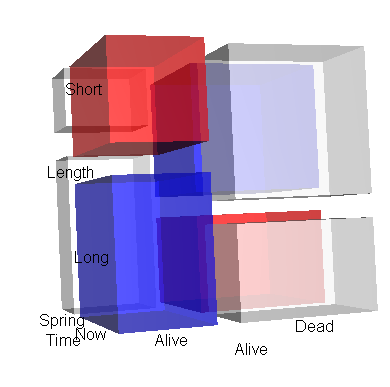
\includegraphics[width=0.6\textwidth]{ch05/fig/mos3d-bartlett.png}
 \caption{3D mosaic plot of the Bartlett data, according to the model of mutual independence}\label{fig:mos3d-bartlett}
\end{figure}

In the view of this figure, it can be seen that cuttings are more likely to be alive
when planted Now and when cut Long. These relations can more easily be
appreciated by rotating the 3D display.
\end{Example}

\DONE{Deleted section on parallel coordinate plots.  Need to fixup \exref{ex:1.7}.}
% \section{Parallel coordinate plots for categorical data}\label{sec:parallel}
% <<sec-parallel, child='ch05/parallel.Rnw'>>=
% @

\section{Visualizing the structure of \loglin models}\label{sec:mosaic-struc}
For quantitative response data, it is easy to visualize a fitted model---
for linear regression, this is just a plot of the fitted line;
for multiple regression or non-linear regression with two predictors,
this is a plot of the fitted response surface.  For a categorical
response variable, an analog of such plots is provided by
effect plots, described later in this book.
\ix{effect plot}

For \ctab data,
mosaic displays can be used in a similar manner to illuminate the relations among
variables in a \ctab represented in various \loglin{} models,
a point described by \citet{TheusLauer:99}.
In fact,
each of the model types depicted in \tabref{tab:hyp3way} has
a characteristic shape and structure in a mosaic display. This,
in turn, leads to a clearer understanding of the structure which appears
in real data when a given model fits, the relations among the models,
and the use of mosaic displays.  The essential idea is a simple
extension of what we do for more traditional models:
show the \emph{expected} (fitted) frequencies under a given model
rather than observed frequencies in a mosaic-like display.

To illustrate, we use some artificial data on the relations among
age, sex and symptoms of some disease shown in the $2 \times 2 \times 2$ table
\code{struc} below.
\begin{knitrout}
\definecolor{shadecolor}{rgb}{1, 0.961, 0.933}\color{fgcolor}\begin{kframe}
\begin{alltt}
\hlstd{> }\hlstd{struc} \hlkwb{<-} \hlkwd{array}\hlstd{(}\hlkwd{c}\hlstd{(}\hlnum{6}\hlstd{,} \hlnum{10}\hlstd{,} \hlnum{312}\hlstd{,} \hlnum{44}\hlstd{,}
\hlstd{+ }                 \hlnum{37}\hlstd{,} \hlnum{31}\hlstd{,} \hlnum{192}\hlstd{,} \hlnum{76}\hlstd{),}
\hlstd{+ } \hlkwc{dim} \hlstd{=} \hlkwd{c}\hlstd{(}\hlnum{2}\hlstd{,} \hlnum{2}\hlstd{,} \hlnum{2}\hlstd{),}
\hlstd{+ } \hlkwc{dimnames} \hlstd{=} \hlkwd{list}\hlstd{(}\hlkwc{Age} \hlstd{=} \hlkwd{c}\hlstd{(}\hlstr{"Young"}\hlstd{,} \hlstr{"Old"}\hlstd{),}
\hlstd{+ }                 \hlkwc{Sex} \hlstd{=} \hlkwd{c}\hlstd{(}\hlstr{"F"}\hlstd{,} \hlstr{"M"}\hlstd{),}
\hlstd{+ }                 \hlkwc{Disease} \hlstd{=} \hlkwd{c}\hlstd{(}\hlstr{"No"}\hlstd{,} \hlstr{"Yes"}\hlstd{))}
\hlstd{+ } \hlstd{)}
\hlstd{> }\hlstd{struc} \hlkwb{<-} \hlkwd{as.table}\hlstd{(struc)}
\hlstd{> }\hlkwd{structable}\hlstd{(Sex} \hlopt{+} \hlstd{Age} \hlopt{~} \hlstd{Disease, struc)}
\end{alltt}
\begin{verbatim}
        Sex     F         M    
        Age Young Old Young Old
Disease                        
No              6  10   312  44
Yes            37  31   192  76
\end{verbatim}
\end{kframe}
\end{knitrout}

First, note that there are substantial associations in this table, as shown in
\figref{fig:struc-mos1}, fitting the (default) mutual independence model.
\begin{knitrout}
\definecolor{shadecolor}{rgb}{1, 0.961, 0.933}\color{fgcolor}\begin{kframe}
\begin{alltt}
\hlstd{> }\hlkwd{mosaic}\hlstd{(struc,} \hlkwc{shade} \hlstd{=} \hlnum{TRUE}\hlstd{)}
\end{alltt}
\end{kframe}\begin{figure}[!htbp]

\centerline{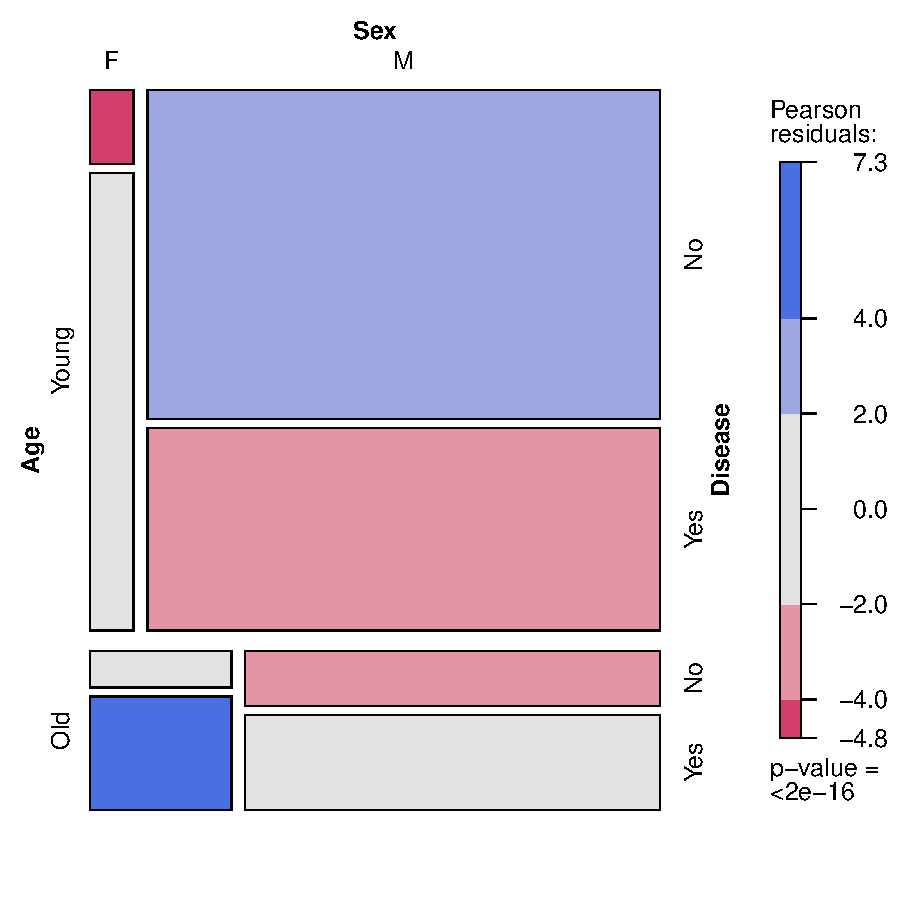
\includegraphics[width=.6\textwidth]{ch05/fig/struc-mos1-1} }

\caption[Mosaic display for the data on age, sex and disease]{Mosaic display for the data on age, sex and disease. Observed frequencies are shown in the plot, and residuals reflect departure from the model of mutual independence.\label{fig:struc-mos1}}
\end{figure}


\end{knitrout}
The first split by \code{Age} shows strong partial
associations between \code{Sex} and \code{Disease} for both young and old.
However the residuals have an opposite pattern for young and old, suggesting
a more complex relationship among these variables.

In this section we are asking a different question: what would mosaic displays look
like if the data were in accord with simpler models?  One way to do this is simply
to use the expected frequencies to construct the tiles, as in sieve diagrams.
The result, in \figref{fig:struc-mos2}, shows that the tiles for sex and disease
align for each of the age groups, but it is harder to see the relations among all
three variables in this plot.

\begin{knitrout}
\definecolor{shadecolor}{rgb}{1, 0.961, 0.933}\color{fgcolor}\begin{kframe}
\begin{alltt}
\hlstd{> }\hlkwd{mosaic}\hlstd{(struc,} \hlkwc{type} \hlstd{=} \hlstr{"expected"}\hlstd{)}
\end{alltt}
\end{kframe}\begin{figure}[!htbp]

\centerline{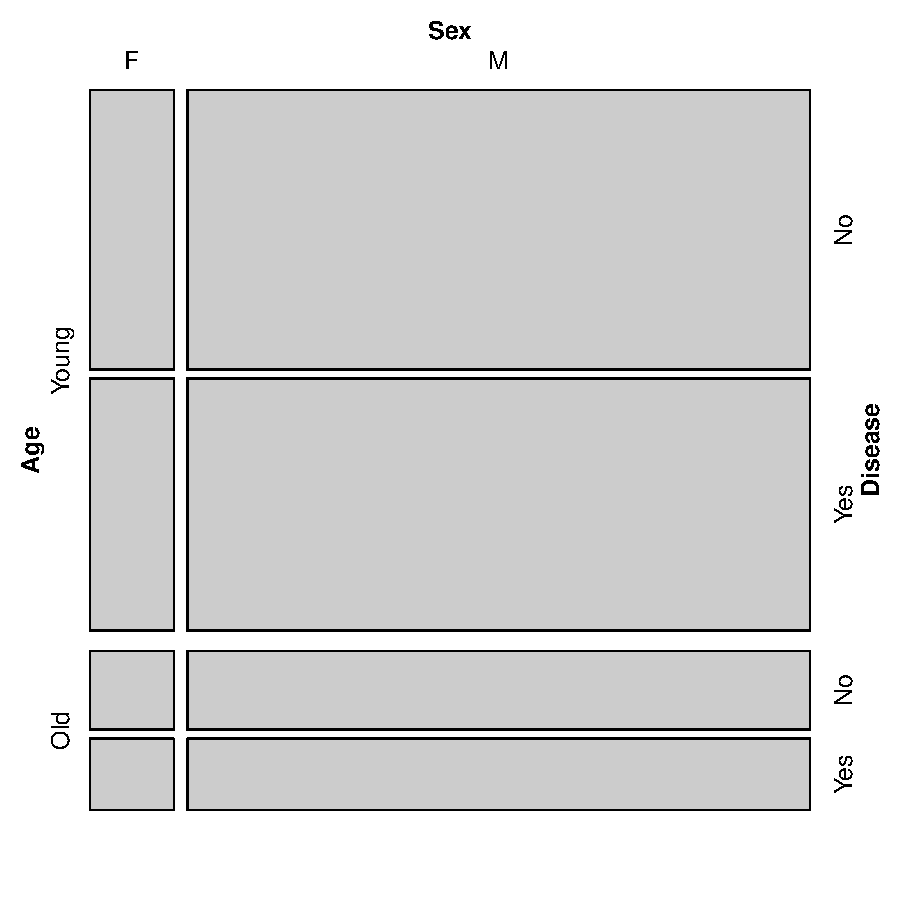
\includegraphics[width=.5\textwidth]{ch05/fig/struc-mos2-1} }

\caption[Mosaic display for the data on age, sex and disease, using expected frequencies under mutual independence]{Mosaic display for the data on age, sex and disease, using expected frequencies under mutual independence.\label{fig:struc-mos2}}
\end{figure}


\end{knitrout}
We can visualize the model-implied relations among all variables together more easily
using mosaic matrices.

\subsection{Mutual independence}
For example, to show the structure of a table which exactly fits the model of
mutual independence, $H_1$, use the \func{loglm} to find the
fitted values, \code{fit}, as shown below.  The
function \func{fitted} extracts these from the \class{loglm} object.

\begin{knitrout}
\definecolor{shadecolor}{rgb}{1, 0.961, 0.933}\color{fgcolor}\begin{kframe}
\begin{alltt}
\hlstd{> }\hlstd{mutual} \hlkwb{<-} \hlkwd{loglm}\hlstd{(}\hlopt{~} \hlstd{Age} \hlopt{+} \hlstd{Sex} \hlopt{+} \hlstd{Disease,} \hlkwc{data} \hlstd{= struc,} \hlkwc{fitted} \hlstd{=} \hlnum{TRUE}\hlstd{)}
\hlstd{> }\hlstd{fit} \hlkwb{<-} \hlkwd{as.table}\hlstd{(}\hlkwd{fitted}\hlstd{(mutual))}
\hlstd{> }\hlkwd{structable}\hlstd{(Sex} \hlopt{+} \hlstd{Age} \hlopt{~} \hlstd{Disease, fit)}
\end{alltt}
\begin{verbatim}
        Sex        F                 M         
        Age    Young      Old    Young      Old
Disease                                        
No           34.0991  10.0365 253.3077  74.5567
Yes          30.7992   9.0652 228.7940  67.3416
\end{verbatim}
\end{kframe}
\end{knitrout}
These fitted frequencies then have the same one-way margins as the
data in \data{struc}, but have no two-way or higher associations.
Then, \func{pairs} for this table, using \code{type="total"}
shows the three-way mosaic for each pair of variables, giving
the result in \figref{fig:struc-mos2}.  We use \code{gp=shading\_Friendly}
to explicitly indicate the zero residuals in the display.


\begin{knitrout}
\definecolor{shadecolor}{rgb}{1, 0.961, 0.933}\color{fgcolor}\begin{kframe}
\begin{alltt}
\hlstd{> }\hlkwd{pairs}\hlstd{(fit,} \hlkwc{gp} \hlstd{= shading_Friendly,} \hlkwc{type} \hlstd{=} \hlstr{"total"}\hlstd{)}
\end{alltt}
\end{kframe}\begin{figure}[!htb]

\centerline{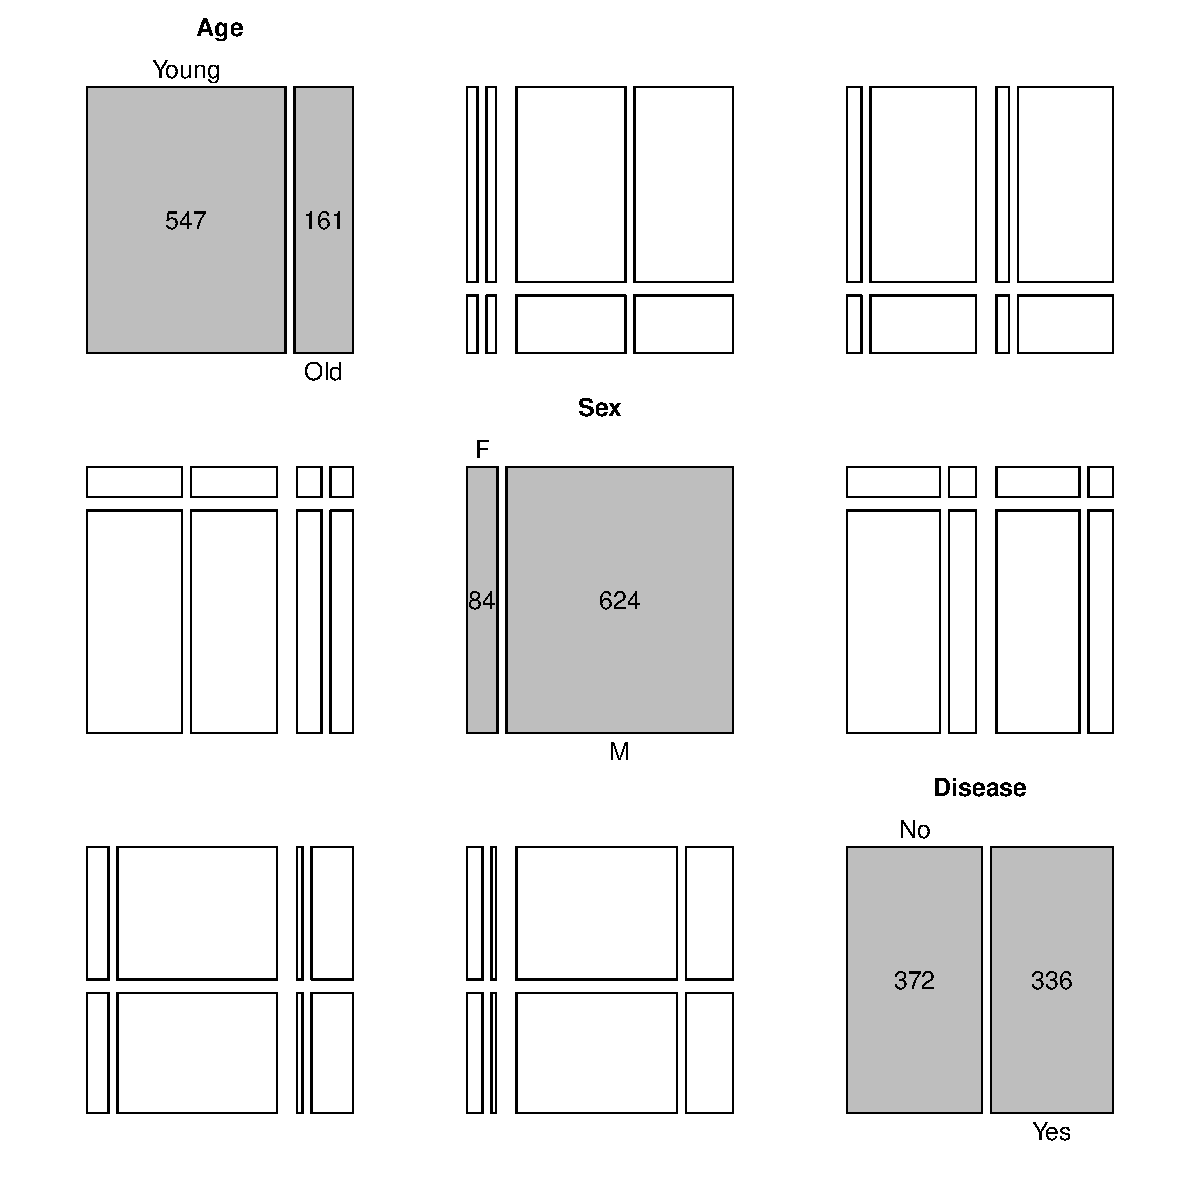
\includegraphics[width=.8\textwidth]{ch05/fig/struc-mos3-1} }

\caption[Mosaic matrix for fitted values under mutual independence]{Mosaic matrix for fitted values under mutual independence.  In all panels the joint frequencies conform to the one-way margins.\label{fig:struc-mos3}}
\end{figure}


\end{knitrout}
In this figure the same data are shown in all the off-diagonal panels
and the mutual independence model was fitted in each case, but with the
table variables permuted.  All residuals are exactly zero in all cells,
by construction.
We see that in each view, the four large
tiles, corresponding to the first two variables align, indicating
that these two variable are marginally independent.
For example, in the (1,2) panel, age and sex are independent, collapsed
over disease.

Moreover, comparing the top half to the bottom half
in any panel we see that the divisions by the third variable
are the same for both levels of the second variable.
In the (1, 2) panel, for example, age and disease are independent
for both males and females.
This means that age and sex are conditionally independent
given disease ($\mathrm{age} \perp \mathrm{sex} \given \mathrm{disease}$).

Because this holds in all six panels, we see that mutual independence
implies that \emph{all pairs} of variables are conditionally
independent, given the remaining one,  ($X \perp Y \given Z$) for all
permutations of variables.  A similar argument can be used to
show that joint independence also holds, i.e., ($(X,Y) \perp Z$) for all
permutations of variables.

Alternatively, you can also visualize these relationships interactively
in a 3D mosaic using \func{mosaic3d}
that allows you to rotate the mosaic to see all views.  In \figref{fig:struct-mos3d1},
all of the 3D tiles are unshaded and you can see that the 3D unit cube has been
sliced according to the marginal frequencies.

\begin{knitrout}
\definecolor{shadecolor}{rgb}{1, 0.961, 0.933}\color{fgcolor}\begin{kframe}
\begin{alltt}
\hlstd{> }\hlkwd{mosaic3d}\hlstd{(fit)}
\end{alltt}
\end{kframe}
\end{knitrout}

\begin{figure}[!htb]
 \centering
 \includegraphics[width=0.6\textwidth]{ch05/fig/struct-mos3d1.png}
 \caption{3D mosaic plot of frequencies according to the model of mutual independence. The one-way margins are
 slices through the unit cube.}\label{fig:struct-mos3d1}
\end{figure}


\subsection{Joint independence}
The model of joint independence, $H_2: \: (A, B) \perp C$, or
equivalently, the \loglin model $[A B][C]$
may be visualized similarly
by a mosaic matrix
in which the data are replaced by fitted values under this model.
We illustrate this for the model [Age Sex][Disease],
calculating the fitted values in a similar way as before.

\begin{knitrout}
\definecolor{shadecolor}{rgb}{1, 0.961, 0.933}\color{fgcolor}\begin{kframe}
\begin{alltt}
\hlstd{> }\hlstd{joint} \hlkwb{<-} \hlkwd{loglm}\hlstd{(}\hlopt{~} \hlstd{Age} \hlopt{*} \hlstd{Sex} \hlopt{+} \hlstd{Disease,} \hlkwc{data} \hlstd{= struc,} \hlkwc{fitted} \hlstd{=} \hlnum{TRUE}\hlstd{)}
\hlstd{> }\hlstd{fit} \hlkwb{<-} \hlkwd{as.table}\hlstd{(}\hlkwd{fitted}\hlstd{(joint))}
\hlstd{> }\hlkwd{structable}\hlstd{(Sex} \hlopt{+} \hlstd{Age} \hlopt{~} \hlstd{Disease, fit)}
\end{alltt}
\begin{verbatim}
        Sex       F               M        
        Age   Young     Old   Young     Old
Disease                                    
No           22.593  21.542 264.814  63.051
Yes          20.407  19.458 239.186  56.949
\end{verbatim}
\end{kframe}
\end{knitrout}

The \func{pairs.table} plot, now using simpler pairwise plots (\code{type="pairwise"}),
is shown in \figref{fig:struc-mos4}.
\begin{knitrout}
\definecolor{shadecolor}{rgb}{1, 0.961, 0.933}\color{fgcolor}\begin{kframe}
\begin{alltt}
\hlstd{> }\hlkwd{pairs}\hlstd{(fit,} \hlkwc{gp} \hlstd{= shading_Friendly)}
\end{alltt}
\end{kframe}\begin{figure}[!htb]

\centerline{\includegraphics[width=.7\textwidth]{ch05/fig/struc-mos4-1} }

\caption[Mosaic matrix for fitted values under joint independence]{Mosaic matrix for fitted values under joint independence for the model [Age Sex][Disease]\label{fig:struc-mos4}}
\end{figure}


\end{knitrout}
This shows, in row 3 and column 3, the anticipated independence of both age and sex with
disease, collapsing over the remaining variable.
The (1,2) and (2,1) panels show that age and sex are still associated
when disease is ignored.

\section{Related visualization methods}\label{sec:related}

A variety of other graphical methods provide the means for visualizing relationships in multiway
frequency tables.  We briefly describe a few of these here, without much detail, to give a sense
of some alternatives.

% <rel-parallel, child="ch05/rel-parallel.Rnw">>=
% @

\subsection{Doubledecker plots}\label{sec:doubledecker}

Doubledecker plots visualize the the dependence of one categorical (typically binary) variable on further categorical variables. Formally, they are mosaic plots with vertical splits for all dimensions (predictors) except the last one, which represents the dependent variable (outcome). The last variable is visualized by horizontal splits, no space between the tiles, and separate colors for the levels. 
They have the advantage of making it easier to ``read'' the differences among the conditional response proportions in relation to combinations of
the explanatory variables. Moreover, for a binary response, the difference in these conditional proportions for any two columns has a direct
relation to the odds ratio for a positive response in relation to those predictor levels \citep{Hofmann:2001}.

The \func{doubledecker} function in \pkg{vcd} takes a formula argument of the form \verb|R ~ E1 + E2 + ...|
where \code{R} is the response variable and \code{E1}, \code{E2}, $\dots$ are the predictors in the
contingency table in array form.  The shorthand notation, \verb|R ~ .| means that all variables other
than \code{R} are taken as predictors, in their order in the array.

\begin{Example}[berkeley-ddecker]{Berkeley admissions}
\figref{fig:berkeley-doubledecker} shows the doubledecker plot for the \data{UCBAdmissions} data.
By default, the levels of the response (\var{Admit}) taken in their order in the array and
shaded to highlight the \emph{last} level (Rejected). We want to highlight Admitted, so we reverse
this dimension in the call below.
\begin{knitrout}
\definecolor{shadecolor}{rgb}{1, 0.961, 0.933}\color{fgcolor}\begin{kframe}
\begin{alltt}
\hlstd{> }\hlkwd{doubledecker}\hlstd{(Admit} \hlopt{~} \hlstd{Dept} \hlopt{+} \hlstd{Gender,} \hlkwc{data}\hlstd{=UCBAdmissions[}\hlnum{2}\hlopt{:}\hlnum{1}\hlstd{,,])}
\end{alltt}
\end{kframe}\begin{figure}[!htbp]

\centerline{\includegraphics[width=\textwidth]{ch05/fig/berkeley-doubledecker-1} }

\caption[Doubledecker plot for the UCBAdmissions data]{Doubledecker plot for the UCBAdmissions data\label{fig:berkeley-doubledecker}}
\end{figure}


\end{knitrout}
In \figref{fig:berkeley-doubledecker}, it is easy to see the effects of both \var{Dept} and \var{Gender} on 
\var{Admit}. Admission rate declines across departments A--E, and within departments, the 
proportion admitted is roughly the same, except for department A, where more female applicants
are admitted.
\end{Example}


\begin{Example}[titanic-ddecker]{Titanic data}
\figref{fig:titanic-doubledecker} shows the doubledecker plot for the \data{Titanic} data. The 
levels of the response (\var{Survived}) are shaded in increasing grey levels, highlighting the
proportions of survival.
\begin{knitrout}
\definecolor{shadecolor}{rgb}{1, 0.961, 0.933}\color{fgcolor}\begin{kframe}
\begin{alltt}
\hlstd{> }\hlkwd{doubledecker}\hlstd{(Survived} \hlopt{~} \hlstd{Class} \hlopt{+} \hlstd{Age} \hlopt{+} \hlstd{Sex, Titanic)}
\end{alltt}
\end{kframe}\begin{figure}[!htbp]

\centerline{\includegraphics[width=\textwidth]{ch05/fig/titanic-doubledecker-1} }

\caption[Doubledecker plot for the Titanic data]{Doubledecker plot for the Titanic data\label{fig:titanic-doubledecker}}
\end{figure}


\end{knitrout}
This order of variables makes it easiest to compare survival of men and women within each age--class combination,
but you can also see that survival of adult women decreases with class, and survival among men was greatest
in first class.  Some additional visualizations of these relationships are illustrated using the
next topic in \exref{ex:titanic-lor}.

\end{Example}

\subsection{Generalized odds ratios}\label{sec:oddsratio}

In \exref{ex:wheeze1}, we used fourfold displays (\figref{fig:coalminer1}) to analyze the odds ratio between
breathlessness and wheeze in coal miners as a function of age.  
\figref{fig:coalminer3} showed that a plot of the odds ratio directly against age
gave a simplified description of this 3-way relationship.

Odds ratios for $2 \times 2$ tables can be generalized to $r \times c$ tables in a variety of
ways, and these can also be calculated for \nway tables by treating all but the first two dimensions as strata.
Plots of these generalized odds ratios can be quite informative, perhaps more so than in the $2 \times 2 \times k$ case.

Consider an $R \times C$ table with frequencies $n_{ij}$.  Then a set of $(R-1)\times(C-1)$
\term{local odds ratio}s, $\theta_{i,j}$, can be calculated as the odds ratios for adjacent pairs of rows and columns
as shown in the left panel of \figref{fig:lor}.

\begin{equation*}
    \theta_{ij} = \frac{n_{ij} / n_{i+1, j}} { n_{i,j+1} / n_{i+1, j+1}}
  	            = \frac{n_{ij} \times n_{i+1, j+1}} { n_{i+1, j} \times n_{i,j+1} } 
\comma \quad 
%i=1, 2, \dots, r-1; j=1, 2, \dots, c-1
{{i=1, 2, \dots, R-1} \atop {j=1, 2, \dots, C-1}}
\period
\end{equation*}
These odds ratios correspond to ``profile contrasts''  (or sequential contrasts or successive differences) for ordered categories.  Similarly, if one row category and one column category (say, the last)
are considered baseline or reference categories,
odds ratios with respect to contrasts with those categories (\figref{fig:lor}, right panel) are defined as
\begin{equation*}
\theta_{ij} = \frac{n_{i,j} \times n_{R,C}}{n_{i,C} \times n_{R,j}}
\comma \quad 
%i=1, 2, \dots, r-1; j=1, 2, \dots, c-1
{{i=1, 2, \dots, R-1} \atop {j=1, 2, \dots, C-1}}
\period
\end{equation*}
Note that all such parameterizations are equivalent, in that one can derive all
other possible odds ratios from any non-redundant set, but substance-driven contrasts will be easier to interpret.

\begin{figure}
  \hfill
    \includegraphics[height=.35\textwidth,keepaspectratio=true]{ch05/fig/lor1} \hfill
    \includegraphics[height=.35\textwidth,keepaspectratio=true]{ch05/fig/lor2}
  \hfill
    \label{fig:lor}
    \caption{Generalized odds ratios for an $R \times C$ table. Left: local odds ratios for adjacent categories. Right: odds ratios
    with respect to a reference category (the last). Each log odds ratio is a contrast of the log frequencies, shown by the cell weights.}
\end{figure}

This calculation is simple in terms of log odds ratios, because it corresponds to a contrast among the log frequencies,
with weights $\pm 1$ for the four relevant cells. For local odds ratios, these are
\begin{equation*}
 \ln( \theta_{ij}) = 
  \left(\begin{array}{rrrr}
  1  & -1 &  -1 & 1
  \end{array}
  \right)
  \ln
	\left(\begin{array}{rrrr}
  n_{ij}  & n_{i+1, j} &  n_{i,j+1} & n_{i+1, j+1}
  \end{array}
  \right)\trans \period
\end{equation*}
Consider an $R \times C \times K_1 \times K_2 \times \dots$ frequency table $n_{ij\cdots}$, with factors
$K_1, K_2 \dots$  taken as strata. Let $\vec{n} = \Vec({n_{ij\cdots}})$ be the $N\times 1$ vectorization
of the frequency table. Then, all log odds ratios and their asymptotic covariance matrix can be calculated as:
\begin{eqnarray*}
\ln (\widehat{\vec{\theta}}) & = & \mat{C} \ln(\vec{n}) \\
\mat{S}  \equiv  \V [\ln (\vec{\theta})] & = & \mat{C} \: \diag{(\vec{n}})^{-1} \: \mat{C}\trans
\end{eqnarray*}
where $\mat{C}$ is an $N$-column matrix containing all zeros, except for 
two $+1$ elements and two $-1$ elements in each row that select the four cells involved in each log lodds ratio.%
\footnote{Some additional theory and applications of generalized odds ratios for ordered variables is given by \citet{Goodman:83}.
\citet{Hofmann:2001} describes some connections between odds ratios, \loglin models, and visual modeling using
doubledecker plots and mosaic plots.
}

The function \func{loddsratio} in \pkg{vcdExtra} calculates these values for the categories of the first two
dimensions of an \nway table, together with their asymptotic covariance matrix. Additional dimensions are treated as strata.
The \func{as.array} and \func{as.data.frame} methods can be used to convert a 
\code{loddsratio} object to a form suitable for plotting or further analysis.

\begin{Example}[punish2]{Corporal punishment data}
\exref{ex:punish} used mosaic displays to describe the relationship between attitude toward corporal punishment of children
in relationship to memory of having experienced that as a child and education and age of the respondent.
Given that \var{attitude} is the response, we could examine the odds ratios among this variable and any one predictor,
treating the other variables as strata.
Continuing the analysis of \exref{ex:punish}, we calculate log odds ratios for
the association of \var{attitude} and \var{memory}, stratified by \var{age} and \var{education}.

\begin{knitrout}
\definecolor{shadecolor}{rgb}{1, 0.961, 0.933}\color{fgcolor}\begin{kframe}
\begin{alltt}
\hlstd{> }\hlkwd{data}\hlstd{(Punishment,} \hlkwc{package}\hlstd{=}\hlstr{"vcd"}\hlstd{)}
\hlstd{> }\hlstd{punish} \hlkwb{<-} \hlkwd{xtabs}\hlstd{(Freq} \hlopt{~} \hlstd{memory} \hlopt{+} \hlstd{attitude} \hlopt{+} \hlstd{age} \hlopt{+} \hlstd{education,} \hlkwc{data} \hlstd{= Punishment)}
\hlstd{> }\hlstd{pun.lor} \hlkwb{<-} \hlkwd{loddsratio}\hlstd{(punish)}
\hlstd{> }\hlstd{pun.lor}
\end{alltt}
\begin{verbatim}
log odds ratios for memory and attitude by age, education 

       education
age     elementary secondary   high
  15-24     -1.770    -0.245  0.379
  25-39     -1.664    -0.437  0.486
  40-       -0.878    -1.368 -1.811
\end{verbatim}
\end{kframe}
\end{knitrout}
The \func{as.data.frame} method converts this to a data frame, and adds standard errors (ASE).
\begin{knitrout}
\definecolor{shadecolor}{rgb}{1, 0.961, 0.933}\color{fgcolor}\begin{kframe}
\begin{alltt}
\hlstd{> }\hlstd{pun.lor.df} \hlkwb{<-} \hlkwd{as.data.frame}\hlstd{(pun.lor)}
\hlstd{> }\hlstd{pun.lor.df}
\end{alltt}
\begin{verbatim}
  memory    attitude   age  education    LOR   ASE
1 yes:no no:moderate 15-24 elementary -1.770 1.047
2 yes:no no:moderate 25-39 elementary -1.664 0.623
3 yes:no no:moderate   40- elementary -0.878 0.263
4 yes:no no:moderate 15-24  secondary -0.245 0.875
5 yes:no no:moderate 25-39  secondary -0.437 0.454
6 yes:no no:moderate   40-  secondary -1.368 0.584
7 yes:no no:moderate 15-24       high  0.379 1.261
8 yes:no no:moderate 25-39       high  0.486 0.705
9 yes:no no:moderate   40-       high -1.811 1.123
\end{verbatim}
\end{kframe}
\end{knitrout}
In this form, we can conveniently plot the log odds ratio (LOR) against \var{age} or \var{education},
using the remaining variable for curves in the plot. Here, we use \func{ggplot}, and take some pains to
also plot standard error bars.  The result is shown in \figref{fig:pun-lor-plot}.

\begin{knitrout}
\definecolor{shadecolor}{rgb}{1, 0.961, 0.933}\color{fgcolor}\begin{kframe}
\begin{alltt}
\hlstd{> }\hlkwd{library}\hlstd{(ggplot2)}
\hlstd{> }\hlstd{limits} \hlkwb{<-} \hlkwd{aes}\hlstd{(}\hlkwc{ymax} \hlstd{= LOR} \hlopt{+} \hlstd{ASE,} \hlkwc{ymin}\hlstd{=LOR} \hlopt{-} \hlstd{ASE)}
\hlstd{> }\hlstd{dodge} \hlkwb{<-} \hlkwd{position_dodge}\hlstd{(}\hlkwc{width}\hlstd{=}\hlnum{0.1}\hlstd{)}
\hlstd{> }
\hlstd{> }\hlkwd{ggplot}\hlstd{(pun.lor.df,} \hlkwd{aes}\hlstd{(}\hlkwc{x}\hlstd{=age,} \hlkwc{y}\hlstd{=LOR,} \hlkwc{group}\hlstd{=education,} \hlkwc{color}\hlstd{=education))} \hlopt{+}
\hlstd{+ }  \hlkwd{geom_point}\hlstd{(}\hlkwc{size}\hlstd{=}\hlnum{3}\hlstd{)} \hlopt{+} \hlkwd{geom_line}\hlstd{(}\hlkwc{size}\hlstd{=}\hlnum{1.5}\hlstd{)} \hlopt{+}
\hlstd{+ }  \hlkwd{geom_errorbar}\hlstd{(limits,} \hlkwc{position}\hlstd{=dodge,} \hlkwc{width}\hlstd{=}\hlnum{0.25}\hlstd{)} \hlopt{+}
\hlstd{+ }  \hlkwd{labs}\hlstd{(}\hlkwc{y}\hlstd{=}\hlstr{"log odds ratio: Attitude | Memory"}\hlstd{)} \hlopt{+}
\hlstd{+ }  \hlkwd{theme_bw}\hlstd{()} \hlopt{+}
\hlstd{+ }  \hlkwd{theme}\hlstd{(}\hlkwc{legend.position} \hlstd{=} \hlkwd{c}\hlstd{(}\hlnum{0.85}\hlstd{,} \hlnum{0.85}\hlstd{),}
\hlstd{+ }        \hlkwc{legend.background} \hlstd{=} \hlkwd{element_rect}\hlstd{(}\hlkwc{fill} \hlstd{=} \hlstr{"gray90"}\hlstd{,} \hlkwc{colour} \hlstd{=} \hlstr{"black"}\hlstd{))}
\end{alltt}
\end{kframe}\begin{figure}[!htbp]

\centerline{\includegraphics[width=.8\textwidth]{ch05/fig/pun-lor-plot-1} }

\caption[Log odds ratio for the association between attitude and memory of corporal punishment, stratified by age and education]{Log odds ratio for the association between attitude and memory of corporal punishment, stratified by age and education. Error bars show $\pm 1$ standard error.\label{fig:pun-lor-plot}}
\end{figure}


\end{knitrout}
Compared to \figref{fig:punish-cond1}, the differences among the age, education groups are now clear.
For respondents less than age 40, increasing education increases the association (log odds ratio) 
between attitude and memory: those who remembered corporal punishment as a child are more likely to
approve of it as their education increases.  This result is reversed for those over 40, where all
log odds ratios are negative: memory of corporal punishment makes it \emph{less} likely to approve,
and this effect becomes stronger with increased education.

Because log odds ratios have an approximate normal distribution under the null hypothesis that
all $\log \theta_{ij} =0$, you can treat these values as data, and carry out a rough analysis
of the effects of the stratifying variables using ANOVA, with weights inversely proportional to the
estimated sampling variances. In the analysis shown below, we have treated age and education as
ordered (numeric) variables.


\begin{knitrout}
\definecolor{shadecolor}{rgb}{1, 0.961, 0.933}\color{fgcolor}\begin{kframe}
\begin{alltt}
\hlstd{> }\hlstd{pun.mod} \hlkwb{<-} \hlkwd{lm}\hlstd{(LOR} \hlopt{~} \hlstd{age} \hlopt{*} \hlstd{education,} \hlkwc{data}\hlstd{=pun.lor.df,} \hlkwc{weights}\hlstd{=}\hlnum{1}\hlopt{/}\hlstd{ASE}\hlopt{^}\hlnum{2}\hlstd{)}
\hlstd{> }\hlkwd{anova}\hlstd{(pun.mod)}
\end{alltt}
\begin{verbatim}
Analysis of Variance Table

Response: LOR
              Df Sum Sq Mean Sq F value Pr(>F)  
age            1   1.04    1.04    2.72  0.160  
education      1   1.84    1.84    4.79  0.080 .
age:education  1   5.04    5.04   13.13  0.015 *
Residuals      5   1.92    0.38                 
---
Signif. codes:  0 '***' 0.001 '**' 0.01 '*' 0.05 '.' 0.1 ' ' 1
\end{verbatim}
\end{kframe}
\end{knitrout}
\end{Example}

\begin{Example}[titanic-lor]{Titanic data}
For the \data{Titanic}, it is useful to examine the odds ratios for survival in relation to age or sex, using the
remaining variables as strata. 

For survival and age, we need to permute the dimensions to place these variables as the first two dimensions,
using \func{aperm}.  As well, we reverse the order of the levels so that \code{Survived=="Yes"} and
\code{Age=="Adult"} are first.  The values calculated below then give the log odds of survival for an
adult compared to a child in the combinations sex and class.
\begin{knitrout}
\definecolor{shadecolor}{rgb}{1, 0.961, 0.933}\color{fgcolor}\begin{kframe}
\begin{alltt}
\hlstd{> }\hlstd{titanic.lor1} \hlkwb{<-} \hlkwd{loddsratio}\hlstd{(}\hlkwd{aperm}\hlstd{(Titanic[,,}\hlnum{2}\hlopt{:}\hlnum{1}\hlstd{,}\hlnum{2}\hlopt{:}\hlnum{1}\hlstd{]))}
\hlstd{> }\hlstd{titanic.lor1}
\end{alltt}
\begin{verbatim}
log odds ratios for Survived and Age by Sex, Class 

        Class
Sex          1st     2nd       3rd    Crew
  Male   -3.1210 -5.5015 -0.668740 -1.2479
  Female  2.3425 -1.5103  0.031104  1.7677
\end{verbatim}
\end{kframe}
\end{knitrout}
Similarly, for survival and sex, we obtain the log odds ratios of survival for males versus females,
for the combinations of age and class.%
\footnote{
One complication should be noted here.  When there are zero frequencies in the table
\func{loddsratio} adds 0.5 to each cell by default to avoid problems of division by 0.
There were no children in the crew, so the value 0.000 reported there should be
taken as \code{NA}.
}
\begin{knitrout}
\definecolor{shadecolor}{rgb}{1, 0.961, 0.933}\color{fgcolor}\begin{kframe}
\begin{alltt}
\hlstd{> }\hlstd{titanic.lor2} \hlkwb{<-} \hlkwd{loddsratio}\hlstd{(}\hlkwd{aperm}\hlstd{(Titanic[,,,}\hlnum{2}\hlopt{:}\hlnum{1}\hlstd{],} \hlkwd{c}\hlstd{(}\hlnum{4}\hlstd{,}\hlnum{2}\hlstd{,}\hlnum{3}\hlstd{,}\hlnum{1}\hlstd{)))}
\hlstd{> }\hlstd{titanic.lor2}
\end{alltt}
\begin{verbatim}
log odds ratios for Survived and Sex by Age, Class 

       Class
Age         1st      2nd      3rd    Crew
  Child  1.2993 -0.16034 -0.77879  0.0000
  Adult -4.1643 -4.15161 -1.47864 -3.0156
\end{verbatim}
\end{kframe}
\end{knitrout}

These two tables of log odds ratios can be plotted using \func{ggplot} using code analogous to that shown
in \exref{ex:punish2}.  The result is shown in \figref{fig:titanic-lor-plot} for both tables
(suppressing the point for children in the crew as footnoted above).
\begin{knitrout}
\definecolor{shadecolor}{rgb}{1, 0.961, 0.933}\color{fgcolor}\begin{figure}[!htbp]

\centerline{\includegraphics[width=0.49\textwidth]{ch05/fig/titanic-lor-plot-1} 
\includegraphics[width=0.49\textwidth]{ch05/fig/titanic-lor-plot-2} }

\caption[Log odds ratio plots for the Titanic data.]{Log odds ratio plots for the Titanic data. Left: Odds ratios for survival and age, by sex and class. Right: for survival and sex, by age and class. Error bars show $\pm 1$ standard error.\label{fig:titanic-lor-plot}}
\end{figure}


\end{knitrout}
In the left panel of \figref{fig:titanic-lor-plot} you can see that the odds ratio of
survival for adults relative to children was always greater for females as compared
to males, but much less so in 3$^{rd}$ class.
In the right panel, the odds ratio of survival for males versus females was always
greater for children than adults, again less so in 3$^{rd}$ class.
\end{Example}

Other examples and plots for log odds ratios are shown in \help{loddsratio}.


\section{Chapter summary}\label{sec:mosaic-summary}
%\section{Chapter summary}
\begin{itemize}
\item The mosaic display depicts the frequencies in a \ctab{} by a collection of rectangular ``tiles''
whose area is proportional to the cell frequency.
The residual from a specified model is portrayed by shading the tile
to show the sign and magnitude of the deviation from the model.

\item For two-way tables, the tiles for the second variable align
at each level of the first variable when the two variables are independent
(see \figref{fig:UKsoccer-mosaic}).

\item The perception and understanding of \emph{patterns of association}
(deviations from independence) are enhanced by reordering the
rows or columns to give the shading of the residuals a more
coherent pattern.  An opposite-corner pattern ``explains''
the association in terms of the ordering of the factor levels.

\item For three-way and larger tables, a variety of models can be fit
and visualized.
Starting with a minimal baseline model, the pattern of residuals
will often suggest additional terms which must be added to
``clean the mosaic.''

\item It is often useful to examine the \emph{sequential} mosaic
displays for the marginal subtables with the variables in a given order.
Sequential models of joint independence provide a breakdown of the
total association in the full table, and are particularly
appropriate when the last variable is a response.

\item Partial association, which refers to the associations among
a subset of variables, within the levels of other variables,
may be easily studied by constructing separate mosaics for the subset
variables for the levels of the other, ``given'' variables.
These displays provide a breakdown of a model of conditional association
for the whole table, and serve as an analog of coplots for quantitative
data.

\item Mosaic matrices, consisting of all pairwise plots of an $n$-way
table, provide a way to visualize all marginal, joint, or conditional 
relations simultaneously.  Parallel set plots provide another method
to visualize \nway tables.

\item The structural relations among model terms in various \loglin
models themselves can also be visualized by mosaic matrices
showing the expected, rather than observed, frequencies under different
models.
\end{itemize}



\section{Further reading}\label{sec:mosaic-reading}

\section{Lab exercises}\label{sec:mosaic-lab}


\begin{Exercises}

\exercise The data set \data{criminal} in the package \pkg{logmult} gives the
$4 \times 5$ table below of the
number of men aged 15-19 charged with a criminal case for whom charges were dropped
in Denmark from 1955--1958.
\begin{knitrout}
\definecolor{shadecolor}{rgb}{1, 0.961, 0.933}\color{fgcolor}\begin{kframe}
\begin{alltt}
\hlstd{> }\hlkwd{data}\hlstd{(}\hlstr{"criminal"}\hlstd{,} \hlkwc{package}\hlstd{=}\hlstr{"logmult"}\hlstd{)}
\hlstd{> }\hlstd{criminal}
\end{alltt}
\begin{verbatim}
      Age
Year    15  16  17  18  19
  1955 141 285 320 441 427
  1956 144 292 342 441 396
  1957 196 380 424 462 427
  1958 212 424 399 442 430
\end{verbatim}
\end{kframe}
\end{knitrout}
  \begin{enumerate*}
    \item Use \func{loglm} to test whether there is an association between \var{Year}
    and \var{Age}.  Is there evidence that dropping of charges in relation to
    age changed over the years recorded here?
    \item Use \func{mosaic} with the option \code{shade=TRUE} to display the
    pattern of signs and magnitudes of the residuals.  Compare this with the
    result of \func{mosaic} using ``Friendly shading,'' from
    the option \code{gp=shading\_Friendly}.  Describe verbally what you see
    in each regarding the pattern of association in this table.
  \end{enumerate*}

\exercise The \Rpackage{Lahman} contains comprehensive data on baseball statistics for Major League Baseball from 1871 through 2012.  
For all players, the \data{Master} table records the handedness of players, in terms of
throwing (L, R) and batting (B, L, R), where B indicates ``both.''
The table below was generated using the following code:
\begin{knitrout}
\definecolor{shadecolor}{rgb}{1, 0.961, 0.933}\color{fgcolor}\begin{kframe}
\begin{alltt}
\hlstd{> }\hlkwd{library}\hlstd{(Lahman)}
\hlstd{> }\hlkwd{data}\hlstd{(}\hlstr{"Master"}\hlstd{,} \hlkwc{package}\hlstd{=}\hlstr{"Lahman"}\hlstd{)}
\hlstd{> }\hlstd{basehands} \hlkwb{<-} \hlkwd{with}\hlstd{(Master,} \hlkwd{table}\hlstd{(throws, bats))}
\end{alltt}
\end{kframe}
\end{knitrout}


% latex table generated in R 3.0.1 by xtable 1.7-1 package
% Thu Feb 27 12:56:12 2014
\begin{table}[ht]
\centering
\begin{tabular}{rrrr}
  \hline
       & \multicolumn{3}{c}{Bats} \\
Throws & B & L & R \\ 
  \hline
  L & 177 & 2640 & 527 \\ 
  R & 924 & 1962 & 10442 \\ 
   \hline
\end{tabular}
\end{table}
  \begin{itemize*}
    \item Use the code above, or else enter these data into a frequency table in \R.
    \item Construct mosaic displays showing the relation of batting and throwing handedness, split first by batting and by throwing.
    \item From these displays, what can be said about players who throw with their left
    or right hands in terms of their batting handedness? 
  \end{itemize*}

\exercise\hard
A related analysis concerns differences in throwing handedness among baseball players
according to the fielding position they play.  The following code calculates a
such a frequency table.

\begin{knitrout}
\definecolor{shadecolor}{rgb}{1, 0.961, 0.933}\color{fgcolor}\begin{kframe}
\begin{alltt}
\hlstd{> }\hlkwd{library}\hlstd{(Lahman)}
\end{alltt}


{\ttfamily\noindent\bfseries\color{errorcolor}{Error in library(Lahman): there is no package called 'Lahman'}}\begin{alltt}
\hlstd{> }\hlstd{MasterFielding} \hlkwb{<-} \hlkwd{data.frame}\hlstd{(}\hlkwd{merge}\hlstd{(Master, Fielding,} \hlkwc{by}\hlstd{=}\hlstr{"playerID"}\hlstd{))}
\end{alltt}


{\ttfamily\noindent\bfseries\color{errorcolor}{Error in merge(Master, Fielding, by = "{}playerID"{}): object 'Master' not found}}\begin{alltt}
\hlstd{> }\hlstd{throwPOS} \hlkwb{<-} \hlkwd{with}\hlstd{(MasterFielding,} \hlkwd{table}\hlstd{(POS, throws))}
\end{alltt}


{\ttfamily\noindent\bfseries\color{errorcolor}{Error in with(MasterFielding, table(POS, throws)): object 'MasterFielding' not found}}\end{kframe}
\end{knitrout}
  \begin{enumerate*}
    \item Make a mosaic display of throwing hand vs. fielding position.
    \item Calculate the percentage of players throwing left-handed by position.
    Make a sensible graph of this data.
    \item Re-do the mosaic display with the positions sorted by percentage of left-handers.
    \item Is there anything you can say about positions that have very few left-handed
    players?
  \end{enumerate*}


\exercise For the \data{Bartlett} data described in \exref{ex:bartlett}, fit the model of no three-way
association, $H_4$ in \tabref{tab:hyp3way}. 
  \begin{enumerate*}
  \item Summarize the goodness of fit for this model, and compare to simpler models that
  omit one or more of the two-way terms.
  \item Use a mosaic-like display to show the lack of fit for this model.
  \end{enumerate*}

\exercise Red core disease, caused by a fungus, is not something you want if you are a strawberry.
The data set \data{jansen.strawberry} from the \Rpackage{agridat} gives a frequency data
frame of counts of damage from this fungus from a field experiment reported by
\cite{Jansen:1990}. See the help file for details.  The following lines create a
a $3 \times 4 \times 3$ table of crossings of 3 male parents with 4 (different)
female parents, recording the number of plants in four blocks of 9 or 10 plants
each showing red core disease in three ordered categories, C1, C2 or C3.
\begin{knitrout}
\definecolor{shadecolor}{rgb}{1, 0.961, 0.933}\color{fgcolor}\begin{kframe}
\begin{alltt}
\hlstd{> }\hlkwd{data}\hlstd{(}\hlstr{"jansen.strawberry"}\hlstd{,} \hlkwc{package}\hlstd{=}\hlstr{"agridat"}\hlstd{)}
\hlstd{> }
\hlstd{> }\hlstd{dat} \hlkwb{<-} \hlstd{jansen.strawberry}
\hlstd{> }\hlstd{dat} \hlkwb{<-} \hlkwd{transform}\hlstd{(dat,} \hlkwc{category}\hlstd{=}\hlkwd{ordered}\hlstd{(category,} \hlkwc{levels}\hlstd{=}\hlkwd{c}\hlstd{(}\hlstr{'C1'}\hlstd{,}\hlstr{'C2'}\hlstd{,}\hlstr{'C3'}\hlstd{)))}
\hlstd{> }\hlkwd{levels}\hlstd{(dat}\hlopt{$}\hlstd{male)} \hlkwb{<-} \hlkwd{paste0}\hlstd{(}\hlstr{"M"}\hlstd{,} \hlnum{1}\hlopt{:}\hlnum{3}\hlstd{)}
\hlstd{> }\hlkwd{levels}\hlstd{(dat}\hlopt{$}\hlstd{female)} \hlkwb{<-} \hlkwd{paste0}\hlstd{(}\hlstr{"F"}\hlstd{,} \hlnum{1}\hlopt{:}\hlnum{4}\hlstd{)}
\hlstd{> }
\hlstd{> }\hlstd{jansen.tab} \hlkwb{<-} \hlkwd{xtabs}\hlstd{(count}\hlopt{~}\hlstd{male} \hlopt{+} \hlstd{female} \hlopt{+} \hlstd{category,} \hlkwc{data}\hlstd{=dat)}
\hlstd{> }\hlkwd{names}\hlstd{(}\hlkwd{dimnames}\hlstd{(jansen.tab))} \hlkwb{<-} \hlkwd{c}\hlstd{(}\hlstr{"Male parent"}\hlstd{,} \hlstr{"Female parent"}\hlstd{,}
\hlstd{+ }                                 \hlstr{"Disease category"}\hlstd{)}
\hlstd{> }\hlkwd{ftable}\hlstd{(jansen.tab)}
\end{alltt}
\end{kframe}
\end{knitrout}
  \begin{enumerate*}
    \item Use \code{pairs(jansen.tab, shade=TRUE)} to display the pairwise associations
    among the three variables.  Describe how disease category appears to vary with male
    and female parent? Why is there no apparent association between male and female parent?
    \item As illustrated in \figref{fig:HE-fill}, use mosaic to prepare a 3-way mosaic
    plot with the tiles colored in increasing shades of some color according to
    disease category.  Describe the pattern of category C3 in relation to male and
    female parent.  (Hint: the \code{highlighting} arguments are useful here.)
    \item With \code{category} as the response variable, the minimal model for
    association is $\LLM{MF,C}$, or \verb|~ 1*2 + 3|.
    Fit this model using \func{loglm} and display the residuals from this model
    with \func{mosaic}. Describe the pattern of lack of fit of this model.
  \end{enumerate*}

  \exercise The data set \data{caith} in \pkg{MASS} gives another
  classic $4 \times 5$ table 
  tabulating hair color and eye color, this for  
  people in Caithness, Scotland, originally from
  \citet{Fisher:1940}.  The data is stored as a data frame of cell frequencies, whose rows are eye colors
  and whose columns are hair colors.
\begin{knitrout}
\definecolor{shadecolor}{rgb}{1, 0.961, 0.933}\color{fgcolor}\begin{kframe}
\begin{alltt}
\hlstd{> }\hlkwd{data}\hlstd{(}\hlstr{"caith"}\hlstd{,} \hlkwc{package}\hlstd{=}\hlstr{"MASS"}\hlstd{)}
\hlstd{> }\hlstd{caith}
\end{alltt}
\begin{verbatim}
       fair red medium dark black
blue    326  38    241  110     3
light   688 116    584  188     4
medium  343  84    909  412    26
dark     98  48    403  681    85
\end{verbatim}
\end{kframe}
\end{knitrout}

  \begin{enumerate*}
    \item The \func{loglm} and \func{mosaic} functions don't understand data in this format, 
    so use \code{Caith <- as.matrix(caith)} 
    to convert to array form.  Examine the result, and use \code{names(dimnames(Caith))<-c()} to
    assign appropriate names to the row and column dimensions.
    \item Fit the model of independence to the resulting matrix using \func{loglm}.
    \item Calculate and display the residuals for this model.
    \item Create a mosaic display for this data.
  \end{enumerate*}
  
%\TODO{Add exercise using \code{vcd::HairEyePlace}}

  \exercise The \data{HairEyePlace} data in \pkg{vcdExtra}, gives similar data on hair color and eye color, for both
  Caithness and Aberdeen as a $4 \times 5 \times 2$ table.
  \begin{enumerate*}
    \item Prepare separate mosaic displays, one for each of Caithness and Aberdeen.  Comment on any difference in
    the pattern of residuals.
    \item Construct condition mosaic plots, using the formula \verb/~Hair+Eye | Place/ and both \func{mosaic} and
    \func{cotabplot}. It is probably more useful here to suppress the legend in these plots.  Comment on the
    difference in what is shown in the two displays.
  \end{enumerate*}
  

  \exercise\label{lab:mosaic-accident} \citet[p. 30--31]{Bertin:83} used a 4-way table of frequencies of traffic accident victims in France in 1958
  to illustrate his scheme for classifying data sets by numerous variables, each of which could have various types
  and could be assigned to various visual attributes. His data are contained in \data{Accident} in \pkg{vcdExtra},
  a frequency data frame representing his $5 \times 2 \times 4 \times 2$ table of the variables
  \var{age}, \var{result} (died or injured), \var{mode} of transportation and \var{gender}.
\begin{knitrout}
\definecolor{shadecolor}{rgb}{1, 0.961, 0.933}\color{fgcolor}\begin{kframe}
\begin{alltt}
\hlstd{> }\hlkwd{data}\hlstd{(}\hlstr{"Accident"}\hlstd{,} \hlkwc{package}\hlstd{=}\hlstr{"vcdExtra"}\hlstd{)}
\hlstd{> }\hlkwd{str}\hlstd{(Accident)}
\end{alltt}
\begin{verbatim}
'data.frame':	80 obs. of  5 variables:
 $ age   : Ord.factor w/ 5 levels "0-9"<"10-19"<..: 5 5 5 5 5 5 5 5 5 5 ...
 $ result: Factor w/ 2 levels "Died","Injured": 1 1 1 1 1 1 1 1 2 2 ...
 $ mode  : Factor w/ 4 levels "4-Wheeled","Bicycle",..: 4 4 2 2 3 3 1 1 4 4 ...
 $ gender: Factor w/ 2 levels "Female","Male": 2 1 2 1 2 1 2 1 2 1 ...
 $ Freq  : int  704 378 396 56 742 78 513 253 5206 5449 ...
\end{verbatim}
\end{kframe}
\end{knitrout}
    \begin{enumerate*}
      \item Use \func{loglm} to fit the model of mutual independence, \verb|Freq ~ age+mode+gender+result| to
      this data.
      \item Use \func{mosaic} to produce an interpretable mosaic plot of the associations among all variables under the
      model of mutual independence.  Try different orders of the variables in the mosaic.  (\emph{Hint}: the 
      \code{abbreviate} component of the 
      \code{labeling\_args} argument to \func{mosaic} will be useful to avoid some overlap of the category labels.)
      \item Treat \var{result} (\code{"Died"} vs. \code{"Injured"}) as the response variable, and fit the model
      \verb|Freq ~ age*mode*gender + result| that asserts independence of \var{result} from all others jointly.
      \item Construct a mosaic display for the residual associations in this model.  Which combinations of the
      predictor factors are more likely to result in death?
    \end{enumerate*}

  \exercise\label{lab:mosaic-vietnam}The data set \data{Vietnam} in \pkg{vcdExtra} gives a $2 \times 5 \times 4$ contingency table in frequency form reflecting a survey of student opinion on the Vietnam War at the University of North Carolina in May 1967.  
  The table variables are sex, year in school and response, which has categories: (A) Defeat North Vietnam by widespread bombing and land invasion; (B) Maintain the present policy; (C) De-escalate military activity, stop bombing and begin negotiations; (D) Withdraw military forces Immediately.  How does the chosen response vary with sex and year?
\begin{knitrout}
\definecolor{shadecolor}{rgb}{1, 0.961, 0.933}\color{fgcolor}\begin{kframe}
\begin{alltt}
\hlstd{> }\hlkwd{data}\hlstd{(}\hlstr{"Vietnam"}\hlstd{,} \hlkwc{package}\hlstd{=}\hlstr{"vcdExtra"}\hlstd{)}
\hlstd{> }\hlkwd{str}\hlstd{(Vietnam)}
\end{alltt}
\begin{verbatim}
'data.frame':	40 obs. of  4 variables:
 $ sex     : Factor w/ 2 levels "Female","Male": 1 1 1 1 1 1 1 1 1 1 ...
 $ year    : int  1 1 1 1 2 2 2 2 3 3 ...
 $ response: Factor w/ 4 levels "A","B","C","D": 1 2 3 4 1 2 3 4 1 2 ...
 $ Freq    : int  13 19 40 5 5 9 33 3 22 29 ...
\end{verbatim}
\end{kframe}
\end{knitrout}
    \begin{enumerate*}
      \item With \var{response} (R) as the outcome variable and \var{year} (Y) and \var{sex} (S) as predictors, the minimal
      baseline \loglin model is the model of joint independence, $\LLM{R,YS}$.  Fit this model, and display it in
      a mosaic plot.
      \item Construct conditional mosaic plots of the \var{response} versus \var{year} separately for males and females.
      Describe the associations seen here.
      \item Follow the methods shown in \exref{ex:employ} to fit separate models of independence for the levels of \var{sex},
      and the model of conditional independence, $R \perp Y \given S$.
      Verify that the decomposition of $\GSQ$ in \eqref{eq:partial1} holds for these models.
      \item Construct a useful 3-way mosaic plot of the data for the model of conditional independence.
    \end{enumerate*}
\end{Exercises}













%%%%%%%%%%%%%%%%%%%%%%%%%%%%%%%%%%%%%%%%%%%%%%%%%%%%%%%%%%%%%%%%%%%%%%%%%


% To resolve citations in the chapter, ...
{\itemsep -1pt
\bibliography{graphics,statistics,timeref,Rpackages}
%%% Use aux2bib to process the .aux file, creating references.bib
%%% Then change to line below
%\bibliography{references}
}

% \newpage
% This document was produced using:
% 
% <<session-info>>=
% print(sessionInfo(), locale = FALSE)
% @

	
%%%%% THE END %%%%%
\end{document}

